%%%%%%%%%%%%%%%%%%%%%%%%%%%%%%%%%%%%%%%%%%%%%%%%%%%%%%%%%%%%
% Template prepared by Dr Daniel Oi, CC BY-NC 4.0          %
%%%%%%%%%%%%%%%%Do Not Alter The Preamble%%%%%%%%%%%%%%%%%%%

%%%%%%%%%%%%%%% Preamble Starts Here %%%%%%%%%%%%%%%%%%%%%%%
%
\documentclass[aps,pra,a4paper,nofootinbib,onecolumn,tightenlines,longbibliography,12pt,amsfonts,amssymb,amsmath,floatfix]{revtex4-2} % Uses the APS RevTeX document class. Versions earlier than 4-2e may not be compatible with the latest LaTeX kernel.
\usepackage{latexsym,graphicx,color,geometry}
\geometry{a4paper, portrait, hmargin=2cm, vmargin={2cm, 2.5cm}}%Defines the page size and margins
\usepackage{url}%Fixes URLs in bibliography
\usepackage{enumitem}%Numbering in Lists
\usepackage[english]{isodate,babel}
\usepackage[figure,table]{totalcount} % counts tables and figures
\usepackage{blindtext} % used to make some example junk text
\usepackage{physics} % very useful for typesetting physics equations
\usepackage{float}
\usepackage{hyperref}

\def\bibsection{\section*{\refname}} %Sorts out reference section and gets rid of horizontal line
\bibliographystyle{acm}
\usepackage{titlesec}
\titleformat*{\section}{\Large\bfseries}
\titleformat*{\subsection}{\large\bfseries}
\titleformat*{\subsubsection}{\normalsize\bfseries\itshape}
\titleformat*{\paragraph}{\large\bfseries}
\titleformat*{\subparagraph}{\large\bfseries}

%%%%Font Definition%%%%
% the document is to be sans serif
\usepackage[T1]{fontenc}
%\usepackage[cmbright]{sfmath}
\usepackage{lmodern}
\renewcommand{\rmdefault}{lmss}
\renewcommand{\sfdefault}{lmss}
\renewcommand{\mathbf}[1]{\ensuremath\textbf{\textit{\textsf{#1}}}}

%%%%%%%%%%%%%%%%%%% Preamble Ends Here %%%%%%%%%%%%%%%%%%%%%%%%


%%%%%%%%%%%%%%%%%%%%%%%%%%%%%%%%%%%%%%%%%%%%%%%%%%%%%%%%%%%%%%%
% Insert any other extra packages or definitions you want here%


%                                                             %
%%%%%%%%%%%%%%%%%%%%%%%%%%%%%%%%%%%%%%%%%%%%%%%%%%%%%%%%%%%%%%%


%%%%%%%%% Fill in your details in the part below %%%%%%%%%
\newcommand{\projecttitle}{Evaluating Spot Finding Methods}% Change title and remove red text color
\newcommand{\studentname}{Anton Gashi}% Type in your name here, but without the red highlighting, same for all other uses of red text
\newcommand{\regnumber}{201914462}
\newcommand{\degree}{MPhys}
\newcommand{\primarysup}{Dr Sebastian van de Linde}
\newcommand{\secondsup}{Dr Daniel Oi}%Comment out this line if not needed
%\newcommand{\thirdsup}{\textcolor{red}{Dr~C~Bloggs}}%Comment out this line if not needed
%%%%%%%%%%%%%%%%%%%%%%%%%%%%%%%%%%%%%%%%%%%%%%



%%%%% Do Not Alter this part %%%%%%%%%%%%
\usepackage{fancyhdr}
\pagestyle{fancy}
\setlength{\headheight}{14pt}
\footskip = 45pt
\fancyhf{}
\lhead{\projecttitle} 
\lfoot{PH450 Report 2021-22}
\cfoot{Student: \regnumber}
\rfoot{Page \thepage}
%%%%%%%%%%%%%%%%%%%%%%%%%%%%%%%%%%%%%%%%%


%%%%%%The document starts here%%%%%%
\begin{document}

%%This section creates the cover page%%

\begin{figure}

\includegraphics[width=\textwidth]{ScienceLogo.png}
\end{figure}

\title{PH450 Report 2021-22\\ \vspace{1cm}
{\huge \projecttitle}\\[0.5cm] %If your title is too long, use \LARGE, \Large, or large instead of \huge
{\footnotesize Submitted in partial fulfilment for the degree of \degree}}

\author{\studentname\\
Registration No.: \regnumber}
\affiliation{SUPA Department of Physics, University of Strathclyde, Glasgow G4 0NG, United Kingdom}

\author{\primarysup{} (Primary Supervisor)}
\noaffiliation
\ifdefined\secondsup % this only appears if \secondsup is set above
\author{\secondsup, (Secondary Supervisor)} % 
\noaffiliation
\fi
\ifdefined\thirdsup
\author{\thirdsup, (Secondary Supervisor)} % 
\noaffiliation
\fi

\date{\today}

\pagenumbering{gobble} % first page in document is not numbered

\maketitle
%%This ends the title page section%%

\newpage % Creates a new page

\pagenumbering{roman} %Use Roman numerals for the front matter pages

\section*{Abstract} %The * suppresses a section number
\addcontentsline{toc}{section}{Abstract}

Sub-pixel localisation and spot finding are methods employed in several different areas of research
like microscopy, small form factor satellites and in some cases LIDAR (Light Detection and Ranging). During this 
project a new method for spot finding was developed and tested against industry standard techniques in order 
to improve accuracy whilst also reduce computational time, this task is in the context of algorithms that need 
to be resource efficient but have improved accuracy compared to previous methods. The method proposed is similar to a Gaussian 
fitting method but with less computational complexity. This method tries to fit a triangle function overtop a spot 
of light that follows a point spread function in order to find the centre of that spot of light. This new method, 
compared to centroiding, was unfortunately marginally less accurate in most applications and much slower also, 
however it does show some promise in places where centroiding usually fails like in high noise situations and 
where box size limitations are a factor. This method shows potential and steps should be carried out 
in order to further the accuracy.

\newpage
\section*{Acknowledgements}
\addcontentsline{toc}{section}{Acknowledgements}

Firstly I would like to thank both my supervisors Dr Sebastian van de Linde and Dr Daniel Oi, 
they were both great at helping, guiding and supporting me through this project. I would also like 
to thank my friends and family who were always there to be relied on if and when needed. 

%%%%%%%%%%%%%%%%%%%%%%%%%%%%%
% Do not alter this section %
\newpage
\tableofcontents % Creates a Table of Contents
\makeatletter
\let\toc@pre\relax
\let\toc@post\relax
\makeatother

\ifnum\totalfigures>0
\newpage
\listoffigures
\addcontentsline{toc}{section}{List of Figures}
\fi

\ifnum\totaltables>0
\newpage
\listoftables
\addcontentsline{toc}{section}{List of Tables}
\fi


% Can edit after here       %
%%%%%%%%%%%%%%%%%%%%%%%%%%%%%


%%%%% Main Report Starts Here %%%%%



\newpage
\pagenumbering{arabic}

\section{Introduction}
\label{sec:intro}
  \subsection{Sub-Pixel Localisation} % (fold)
  \label{sub:spot-finding intro}
  
  Super-resolution microscopy is the process of taking the diffraction limit 
  of a microscope, ~250nm in the x and y direction, and improving it at a minimum by a 
  factor of 2 although more modern methods improve it by up to a factor of 10. In the past this has been achieved by ensemble techniques
  like SIM (Structured Illumination Microscopy) and STED (Stimulated Emission Depletion).
  SIM takes advantage of the moir\'{e} effect which is an interference pattern created by two similar 
  grated patterns that overlap, this produces an apparent pattern. In the case of SIM the patterns are 
  the unknown sample structure emission of the desired object that is being imaged, and the other is 
  a specifically constructed excitation light intensity. These moir\'{e} patterns observed can also be
  much coarser than the grated patterns and may be easily observable in the microscope. \cite{gustafsson2000surpassing}
  An improvement on these methods 
  is single-molecule microscopy, in which molecules are individually fluoresced and 
  imaged instead of ensembles which helps distinguish more detail and produce better
  results than the diffraction limit.
  There are two ways that this general method have been implemented; photo-activated localisation
  microscopy(PALM) and stochastic optical reconstruction microscopy(STORM), both
  rely on fluorophores which are fluorescent chemicals that re-emit light after
  being excited. This helps as the fluorescence emits the light 
  stochastically so only a subset of molecules "light-up" at once, this is important 
  as if they are separated by at least 200nm then they can be located to nanometre precision. 
  Since the molecules are now separated spatially this process needs to just needs to be repeated 
  until all molecules have been "switched-on", this gives a stack of images with blurry spots
  which can be located and recombined into a final image with spot-precision on the order of <~20nm.\cite{galbraith2011super}
  The resolution of a super-resolution image usually doesn't refer to the spot-precision of the 
  located molecule, rather it refers to the structural resolution, this can be calculated along 
  with the density of fluorophores as the Nyquist-Shannon sampling theorem states a minimum number 
  of fluorophores are required to resolve the structure (equation \ref{resolution_equation}). \cite{van2011single}\cite{shannon1949communication}

  \subsubsection{Pixels and Resolution} % (fold)
  \label{ssub:Pixel}
   In the Modern Dictionary of Electronics by Graf a pixel is described as a, 
   spatial resolution element.
   The smallest distinguishable and resolvable area in an image.
   \cite{graf1997modern}
   This was mainly in reference to an analog image but the principle applies 
   to a raster image, which is a $N\cdot M$ matrix of values that display colour and
   intensity. In the specific case of the spot localisation that the Methods section 
   (\ref{sec:Methods}) describe the images are $N\cdot N$ and 16-bit black and white.

   Resolution is the capability of resolving two points or lines.
   Since super-resolution by definition changes the resolution of the input images, 
   the resolution of the output image needs to be quantified.
   Firstly the uncertainty of a spatial measurement is set by the equation;
   \begin{equation}\label{PSFequation}
   \sigma_{x,y}\sim\frac{\sigma_{PSF}}{\sqrt{N}}
   \end{equation}

   Where $\sigma_{PSF}$ is the standard deviation of the point spread function (PSF)
   for the microscope, and $N$ is the number of detected photons per florescent event.
   Since the relationship of equation \ref{PSFequation} is approximately the inverse square root, 
   the more detected photons the lower the uncertainty becomes.\cite{DEMPSEY2013561}
   One of the ways to calculate the maximum resolution achievable is by using the Nyquist-Shannon sampling theorem,
   this states that any detail in a measurement that is smaller than twice the size of the 
   average label to label distance can not reliably be resolved.\cite{tinnefeld2015far}
   The Nyquist resolution limit can be written formally as; 
   \begin{equation}\label{resolution_equation}
     \textrm{Nyquist resolution limit} \/\ =\frac{2}{N^{\frac{1}{D}}}
   \end{equation}

   Where $N$ is the density of labels, and $D$ is the dimensionality. 
   Labels in this specific case refers to each individual fluorescent event that is 
   detected by the camera, the density of labels is sometimes constrained by the 
   molecules being detected as if the structure that's trying to be detected is too
   sparse the uncertainty remains relatively high. 
   For example if the resolution was desired to be 20nm in 
   one dimension then fluorophores have to be separated at least 10nm apart at a density of 
   $~10^4\mu m^{-2}$ at a minimum to achieve it.
   The final resulting uncertainty of any image is therefor the maximum of either equation (\ref{PSFequation}) or (\ref{resolution_equation}). 


   \subsubsection{Fluorophores} % (fold)
   \label{ssub:Fluorophores}
   
   Single molecule super-resolution demands the switching of fluorophores
   stochastically, this can be done reversibly or irreversibly. Reversible switching fluorophores
   are photo-activated and emit light until it becomes non-fluorescent again unless reactivated.  
   Irreversible switching fluorophores either start in the off state or the on state, if it 
   starts in an off state it can be photo-activated and turned on then after a period of 
   time it becomes bleached. If it starts switched on then it can be further excited 
   and transition to a red-shifted state.\cite{van2011single}

   According to equation \ref{resolution_equation} the resolution is increased 
   if the number density $N$ is increased, although in order to locate or find a spot 
   in a diffraction limited image the spots need to be spaced apart. 
   Therefor the rate at which populations are on or off can be denoted by $k_{on}$ and 
   $k_{off}$, also the rate at which the fluorophores switch to the on and off states matter 
   and are denoted as $\tau_{on}$ and $\tau_{off}$. The switch rates are directly linked with 
   how many excitations can be detected at once and thus are linked with the ability to 
   accurately find the location of each spot. Ratios between on and off states are denoted as 
   $r=\frac{k_{off}}{k_{on}}=\frac{\tau_{off}}{\tau_{on}}$, the larger the ratio, r, the more 
   accurate results can be up until a point.
   

  \subsection{Motivation} % (fold)
  \label{sub:Motivation}
  

  The main motivation behind my project is to improve the accuracy of spot finding methods 
  whilst keeping the computational time to a minimum. That is to say this project should be aiming to
  produce a method of spot-finding that either less complex, less computations
  per localisation, fewer steps or a mixture of all. This method will be tested against 
  centroiding, an algorithm known for obtaining good results quickly. Additionally another
  motivation is to create a method that is particularly resistant to background noise. 

  The applications of spot finding reach far beyond localisation microscopy it 
  can be used in other technologies, for example a paper published by Castorena and Creusere \cite{6638050}
  has the problem of needing a fast super-resolution technique to get higher 
  spatial resolution from their LIDAR (Light Detection and Ranging) system. This system is constrained by the 
  laser spot size and precision of the scanning mechanical unit as the single laser 
  source with sampling rates in the GHz range which achieves high accuracy for depth 
  and range resolution but poor spatial resolution. A consideration was to decrease the 
  diameter of the laser thus increasing the spatial sampling density, although this 
  was deemed too computationally expensive.
  
  With the almost exponentially increasing launching of small form factor
  satellites such as the CubeSat, arises the challenge of efficiently utilising
  the satellites computing resources. This means any segment of code being ran on
  the satellite needs to run as quickly as possible whilst keeping a certain
  standard of accuracy, especially for the processes that the satellite depends
  on to operate like attitude control, power management and calculations for
  orbital maneuvers. The main method used for orienting(attitude control) CubSat
  like satellites is by using a Star Tracker, this works by using a camera mounted
  facing stars that are known to the satellite via a star catalogue and moves
  based on how aligned or unaligned a reference image is with the actual image
  seen.\cite{calitz2015design} The method in which the image is processed so it
  can be compared to the reference is called spot finding, this entails taking
  the image and finding each bright spot or star accurately. The motivation for
  this project is to develop a spot finding method for star tracking and compare
  it to the state of the art algorithms measuring accuracy, precision and speed.




\section{Methods} % (fold)
\label{sec:Methods}

  \subsection{Centroiding} % (fold)
  \label{sub:Centroiding_meth}
  
  % subsection subsection name (end)
  
  
  The most common way of spot finding for star tracking is to use centroiding
  algorithms, this is when a subsection of pixels are considered to be a star
  using a rough calculation. The area of interest is then filtered in such a way
  that reduces noise and aberrations, finally apply the algorithm in this case
  it's the centre of gravity method (\ref{eq1})(or the moment
  method)\cite{delabie2014accurate}\cite{stone1989comparison}.
  \begin{equation}\label{eq1}
      (x_b,y_b) = \left( {\frac{\sum_{ij} I_{ij}x_{ij}}{\sum_{ij} I_{ij}},\frac{\sum_{ij} I_{ij}y_{ij}}{\sum_{ij} I_{ij}}}\right)
  \end{equation}
  
  Where $x_{ij}$ and $y_{ij}$ are the x and y co-ordinate components of each pixel, $I_{ij}$ is the intensity 
  value at each pixel and $\sum_{ij}$ is the summation pixel-wise.
  As can be seen in equation \ref{eq1} the centroiding method is fairly trivial, 
  the part that determines the computational operations needed is the i and j terms. 
  These terms are the 'window' of pixels that have been chosen by another rough estimator 
  to get a generalised position, the window is a square around the estimated position so 
  the computation scales like $n^2$, where n is the window size or box size.\cite{stone1989comparison}
  
  \subsection{Fitting methods} % (fold)
  \label{sub:Various fitting methods}

  \subsubsection{Point Spread Function} % (fold)
    \label{ssub:Point Spread Function}
    
    Point Spread Functions(PSF) is the way an object blurs due to the imaging of a point 
    source of light, it is the reason the diffraction limit of a microscope is 250nm (in the
    x,y direction) and >450-700nm (in the z direction).\cite{galbraith2011super} The PSF is also the smallest resolvable
    detail that can be seen with light as other objects that emit light that are smaller than 
    one another all appear to be the same size. Provided that laboratory equipment is set up correctly, 
    i.e. the lens is corrected for aberrations and constants are known such as aperture and angels 
    between lens and samples, methods like the Richards-Wolf model and Gibson-Lanni model will calculate
    the centre of a spot near perfectly. The problem with these methods is that they are complicated and 
    slow, and also offer an answer that is unnecessarily accurate for most applications. \cite{richards1959electromagnetic}\cite{small2014fluorophore}
 

    % subsubsection Point Spread Function (end)
    \subsubsection{Gaussian} % (fold)
    \label{ssub:Gaussian}

    Where the exact prediction of section (\ref{ssub:Point Spread Function}) fails Gaussian fitting tries to succeed 
    by presuming that, if all equipment is set up correctly, the centre of a PSF of a point source is 
    always going to be in the centre. Thus for 2-D spot finding that can't afford the computational time of 
    the previous method uses the more simple equation:
    \begin{equation}\label{Gaussian}
    I(x,y)=I_0\cdot \exp(-a\cdot k^2((x-x_0)^2+(y-y_0)^2))+b
    \end{equation}
    Where k is $\frac{2\pi}{\lambda}$, $a$ is the width of the PSF, $I_0$ is the peak intensity and b is the average background per pixel. \cite{small2014fluorophore}
    A Gaussian fit is going to mostly cover the shape of a point source of light, especially since the airy disk rings on 
    the periphery of the center of the function do not determine the where the center is. 
    
    The Gaussian method usually uses one of two fitting methods, least-squares criterion (LS) or the 
    maximum-likelihood estimation (MLE). \cite{small2014fluorophore} LS equation is as follows: 

    \begin{equation}\label{LS}
      S=\sum_{pixels}\frac{(data-model\;prediction)^2}{expected\;variance\;of\;data}
    \end{equation}

    The error (S) in the LS model is the subtracted difference between the predicted signal and the actual 
    data itself squared, over the expected variance. The expected variance is the variation of the signal 
    of that pixel, meaning if a bad error (S) is obtained that does not necessarily mean a bad prediction was 
    given. Parameters in the Gaussian are altered and the error (S) is minimised to an acceptable amount and thus 
    a fit is then obtained.

    MLE is more complicated and is based on the idea that there is, like the name suggests, a maximum limit for the
    achievable accuracy. This is due to variance in noise, this is why MLE requires a model of the PSF and all 
    forms of noise that the camera has. 

    \subsubsection{Triangular method} % (fold)
    \label{ssub:Triangular method}
    
    The triangle method being used takes inspiration from the Gaussian method, in which,
    a Gaussian curve is produced and the area is calculated by integrating the function. 
    After this the position of the spot is estimated by a hyper-parameter optimisation method 
    which minimises the residual area left over from the fitting process.
    This triangle method looks to reduce the computational load by removing the integration step, 
    this can be done as the area of a triangle is just $\frac{1}{2}\ base\cdot height$. 
    On top of this, the method also sums pixel intensities across axis, firstly it gives a 
    better signal to noise ratio but also it means the triangle only needs to be rendered in 2 dimensions 
    instead of 3, further reducing the computational time. Analogous to equation \ref{Gaussian}, the triangle 
    method function takes three parameters; center, half base and height, from this the three points of a 
    triangle are calculated. The residual seen in figure \ref{fig:visual_test} is calculated 
    similarly to equation \ref{LS} the image data is subtracted from a prediction, then the difference 
    is squared and summed pixel-wise. 

    \begin{equation}\label{residual}
      Residual=\sum_{pixels}(spot\;data-model\;prediction)^2
    \end{equation}

    The optimisation of this method uses a simple grid search to try and 
    find the minimum of equation \ref{residual}.


    \begin{figure}[H]
      \begin{center}
        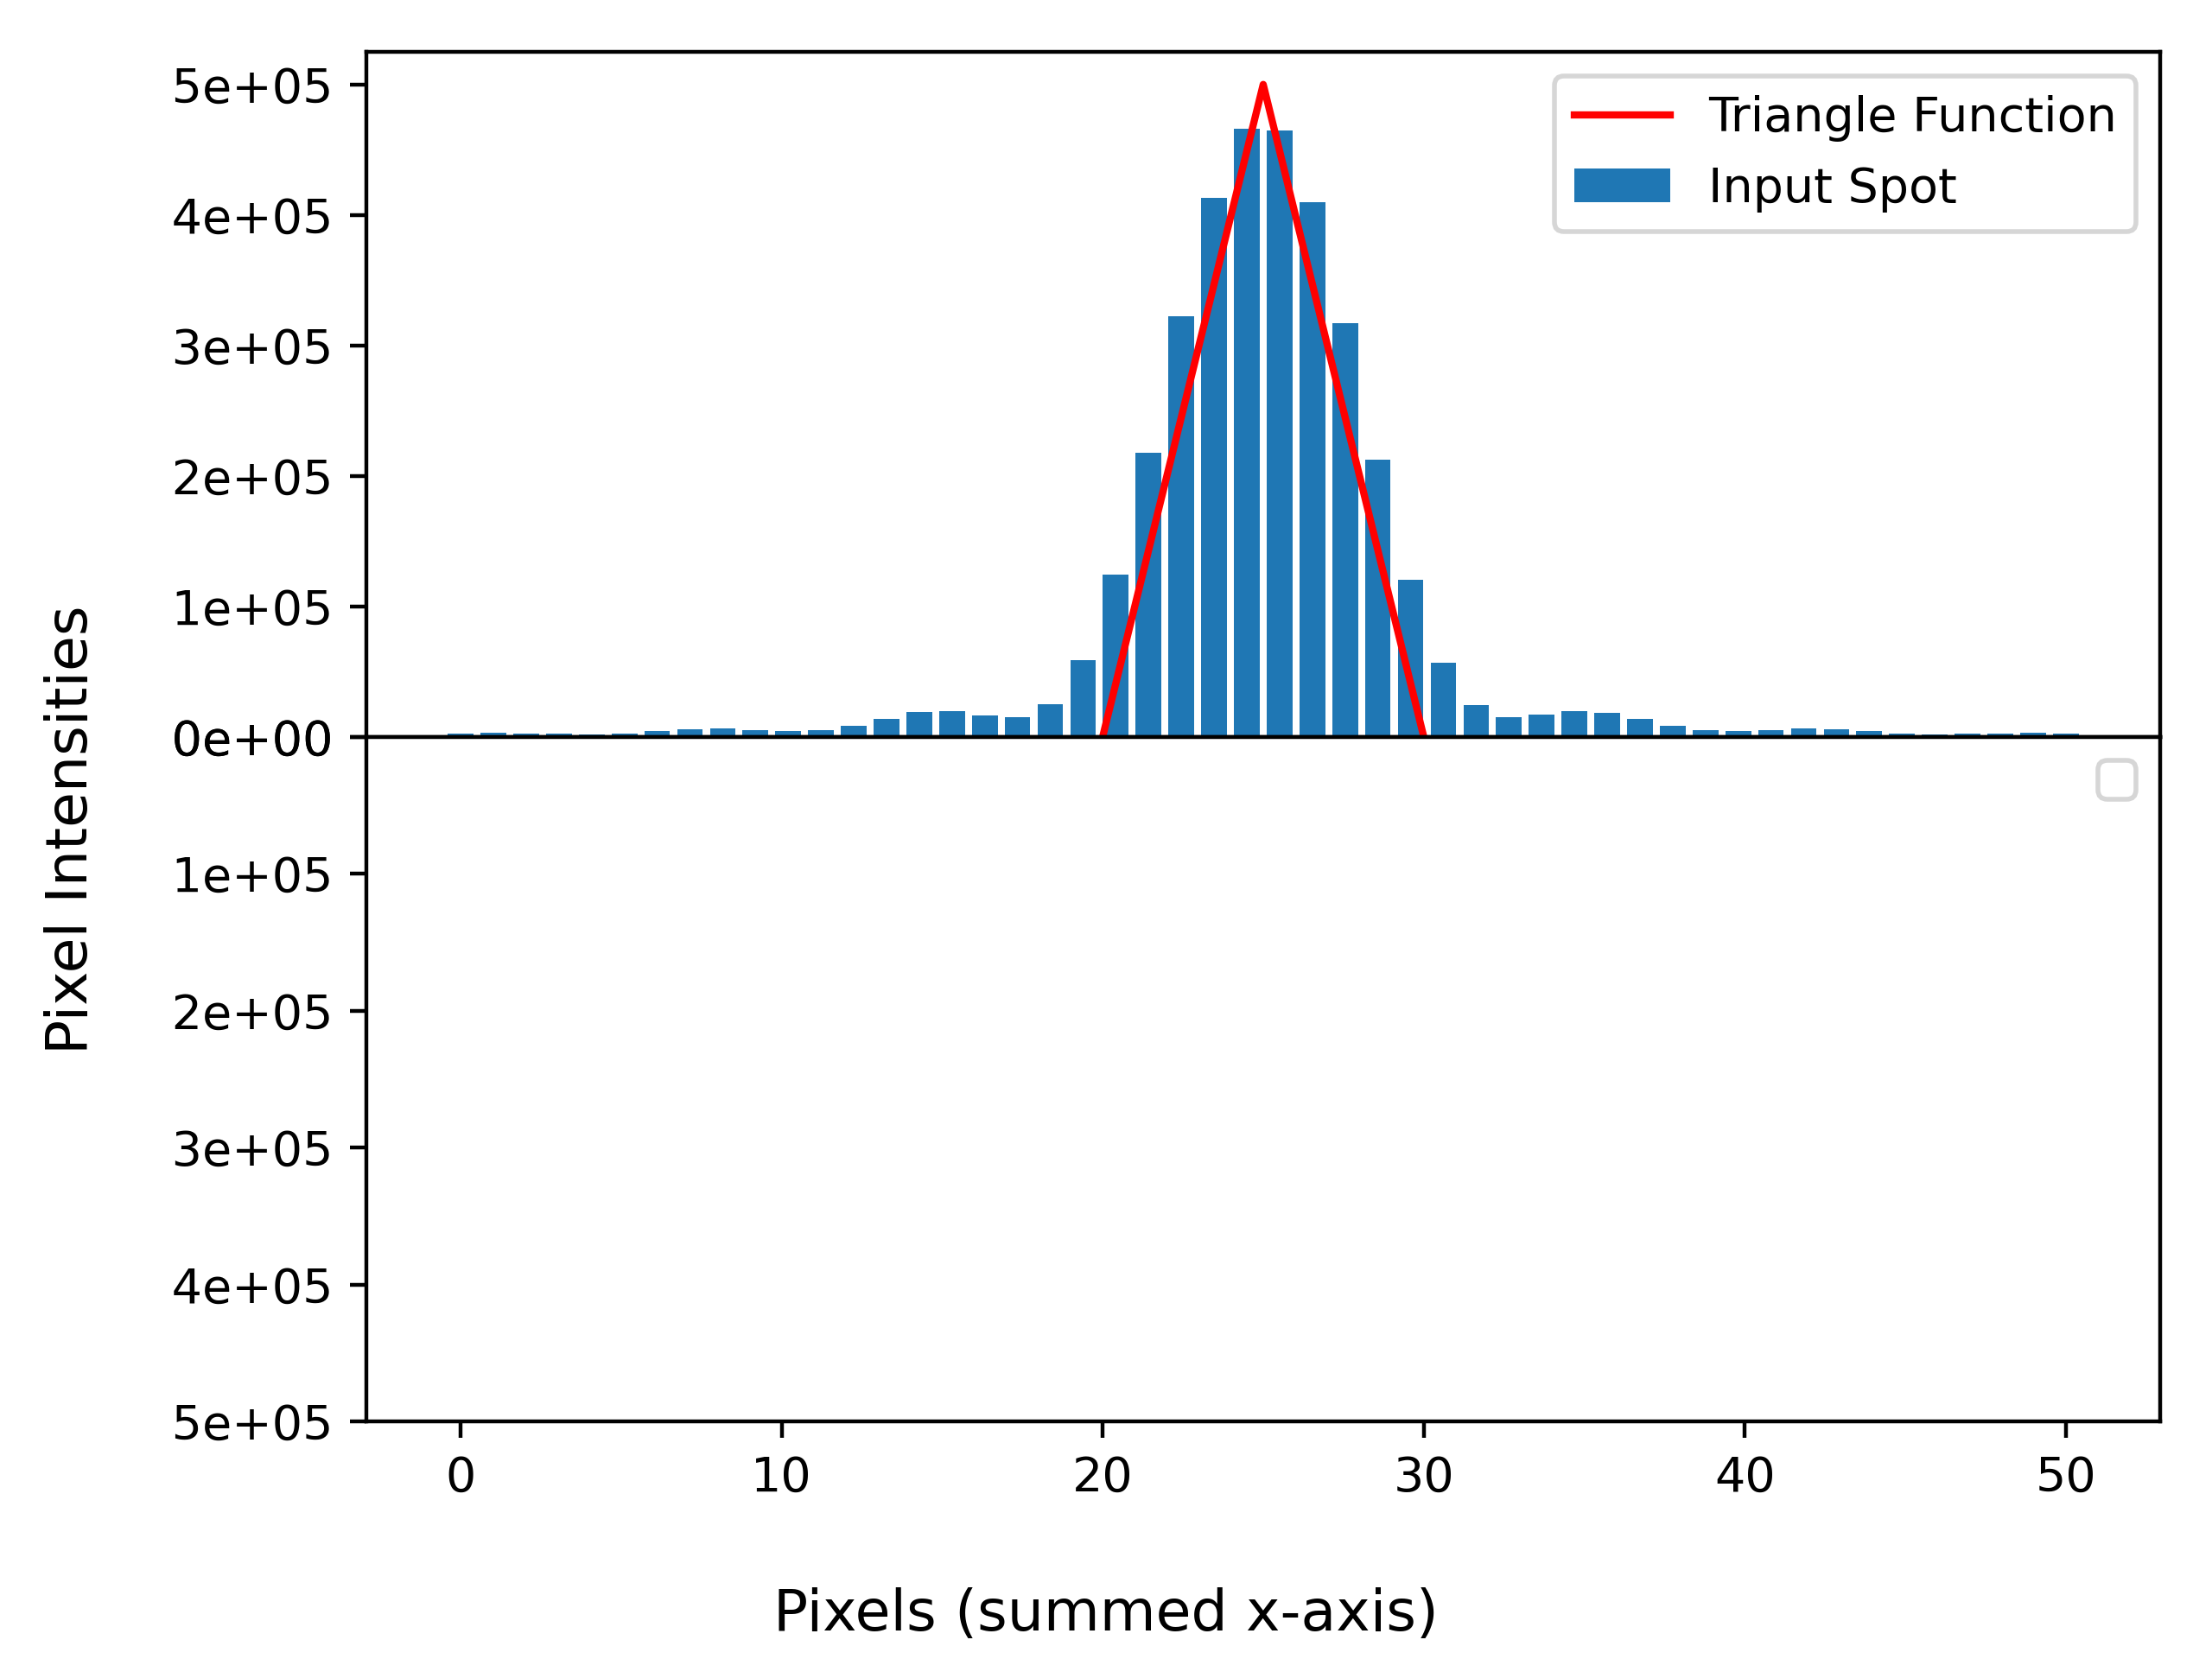
\includegraphics[width=0.6\textwidth]{project_pics/visual_test_2.png}
      \end{center}
      \caption{Graph of ideal spot data}
      \label{fig:visual_test_2}
    \end{figure}

    \begin{figure}[H]
      \begin{center}
        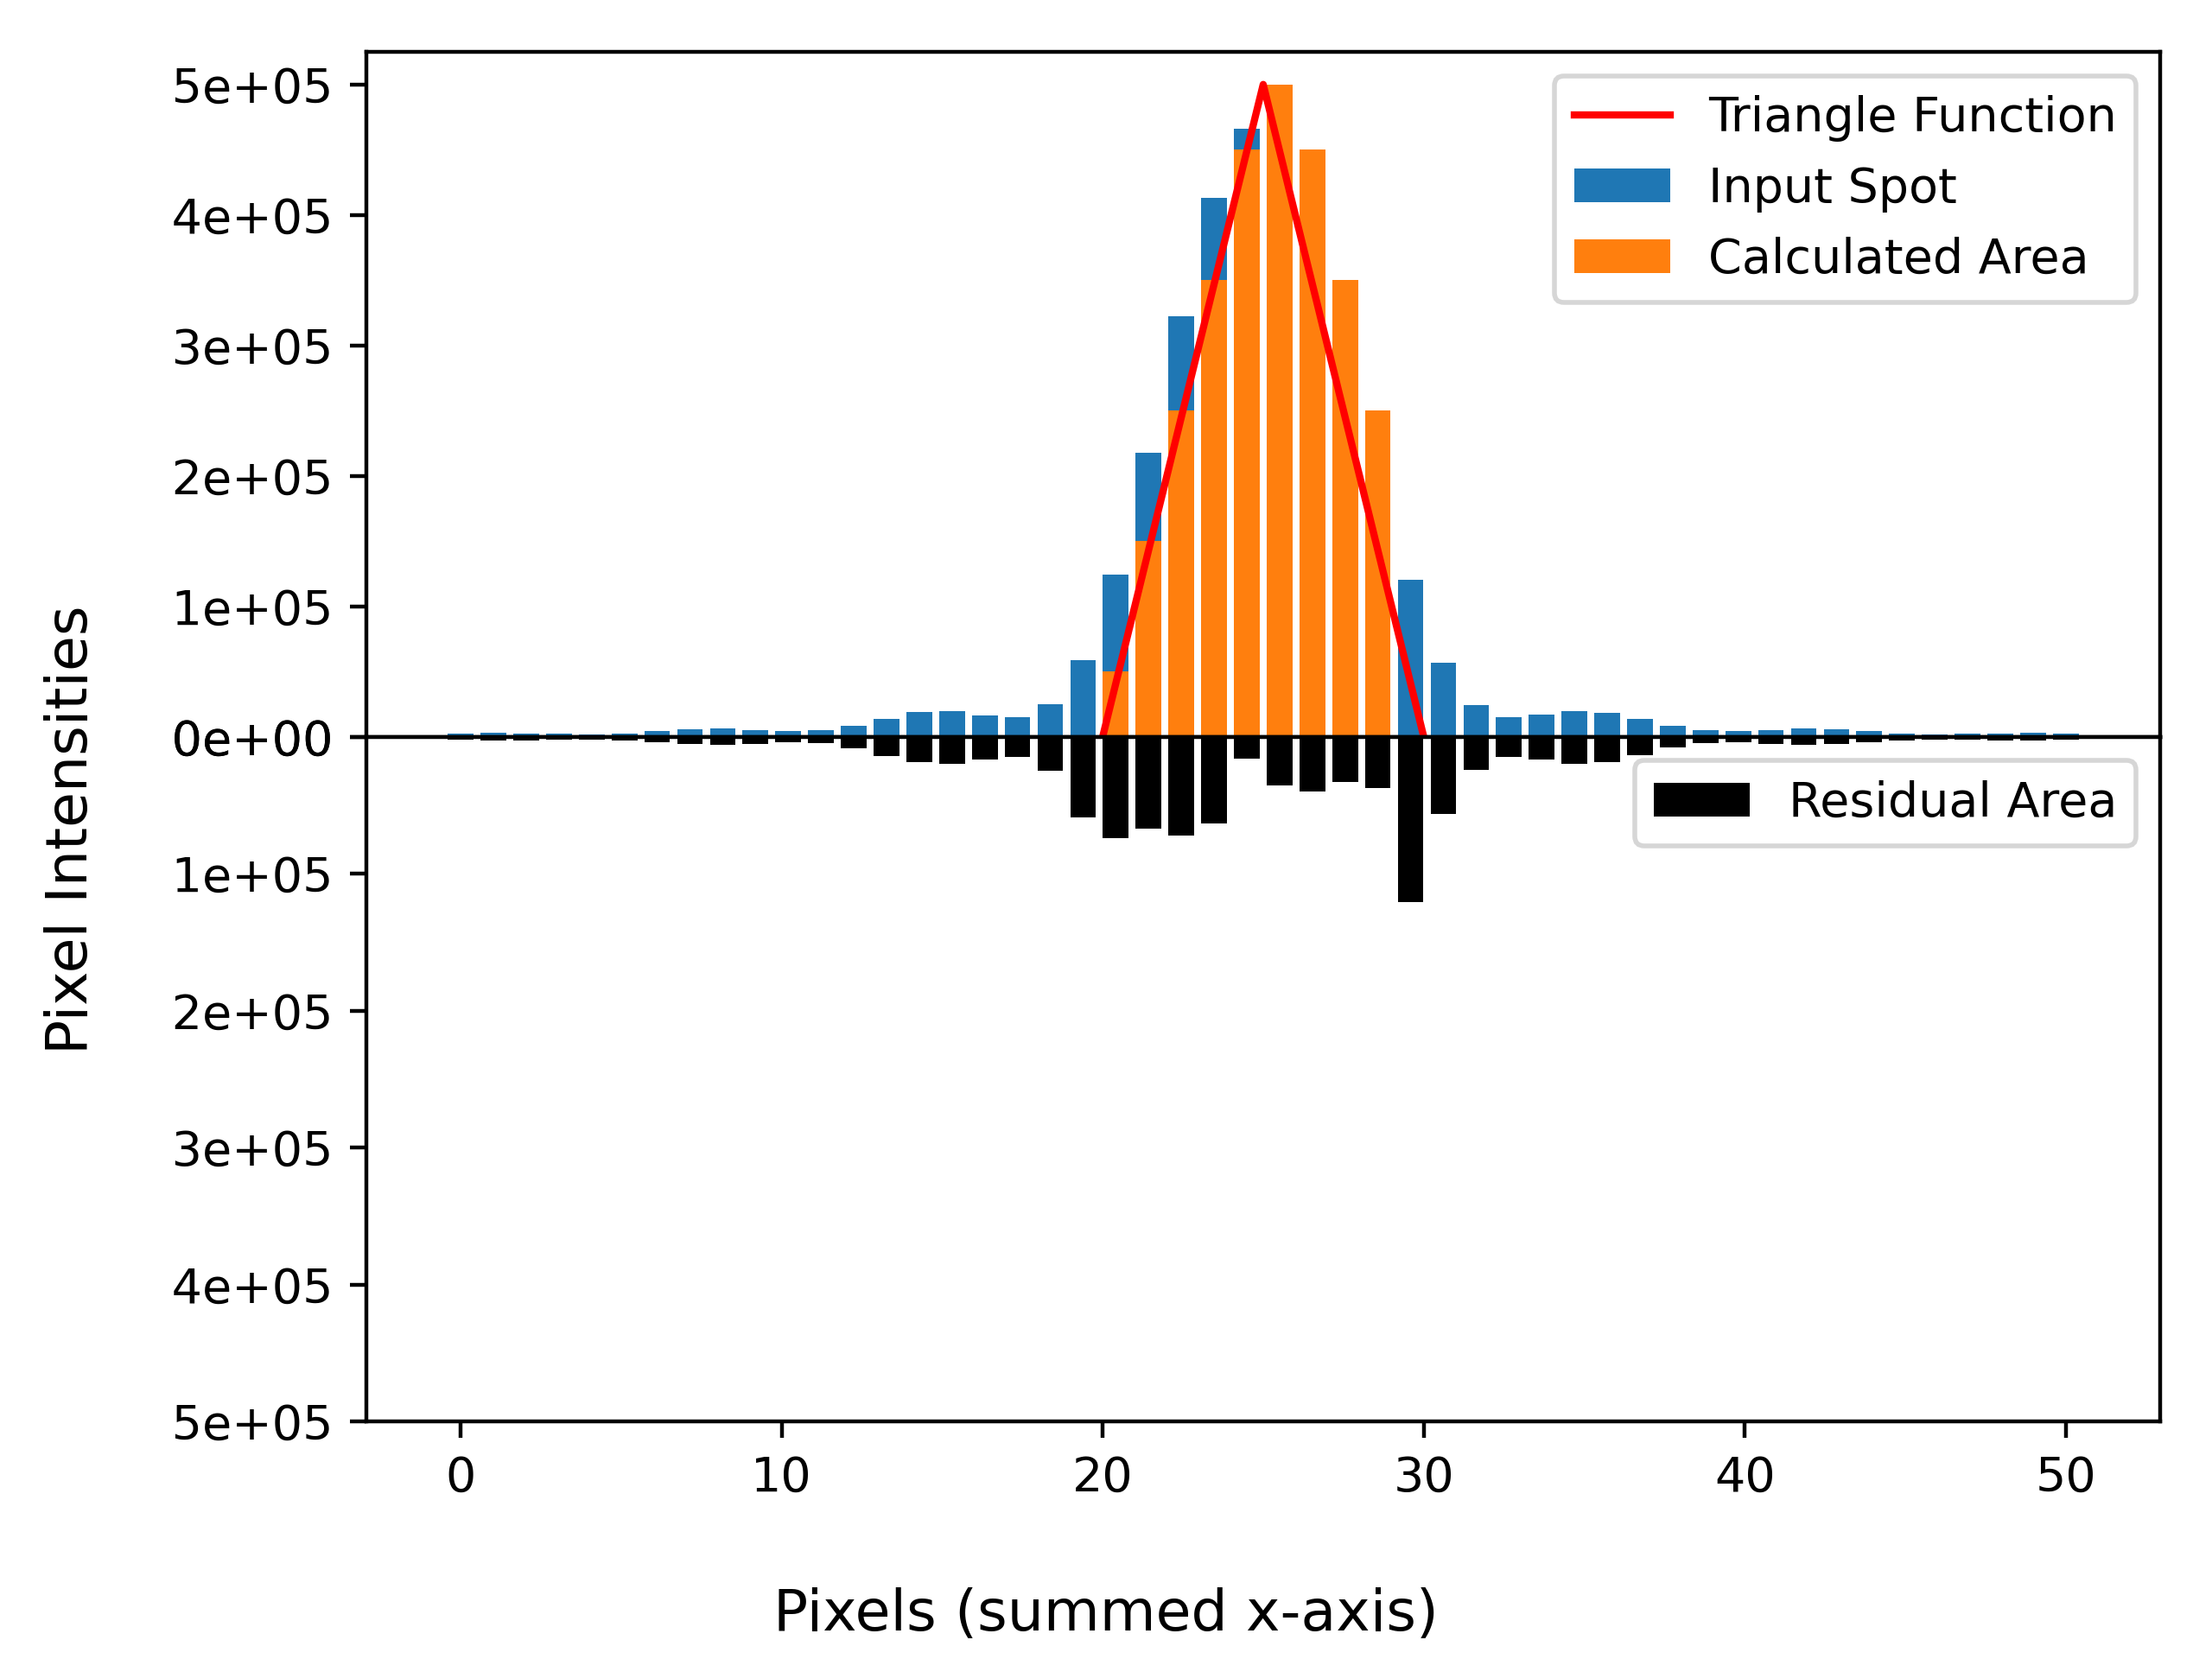
\includegraphics[width=0.6\textwidth]{project_pics/visual_test.png}
      \end{center}
      \caption{Graph of data from figure \ref{fig:visual_test_2} with the calculated area and residual}
      \label{fig:visual_test}
    \end{figure}
    
    As can be seen in figure \ref{fig:visual_test} the area of the simulated spot are subtracted from 
    the area under the triangle and a residual is left over, this residual parameter is the 
    variable to be minimised for in the optimisation routine.

    \begin{figure}[H]
      \begin{center}
        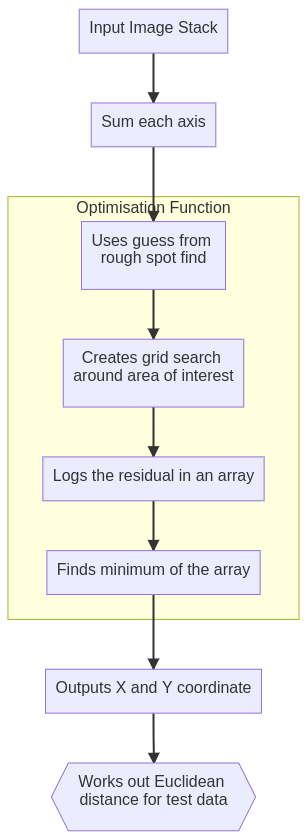
\includegraphics[width=0.4\textwidth]{project_pics/flowchart.png}
      \end{center}
      \caption{Flowchart describing how the code for the triangular fitting method works}
      \label{fig:flowchart}
    \end{figure}
    
    Once the triangle algorithm was implemented it was tested on TIFF stacks of 100 images 
    of perfect spot data. The absolute error (Euclidean distance) was calculated from each 
    axis and plotted as seen in figure \ref{fig:single_histo} A. In image B a histogram 
    was produced so that the spread was more visible.

    \begin{figure}[H]
    \begin{center}
      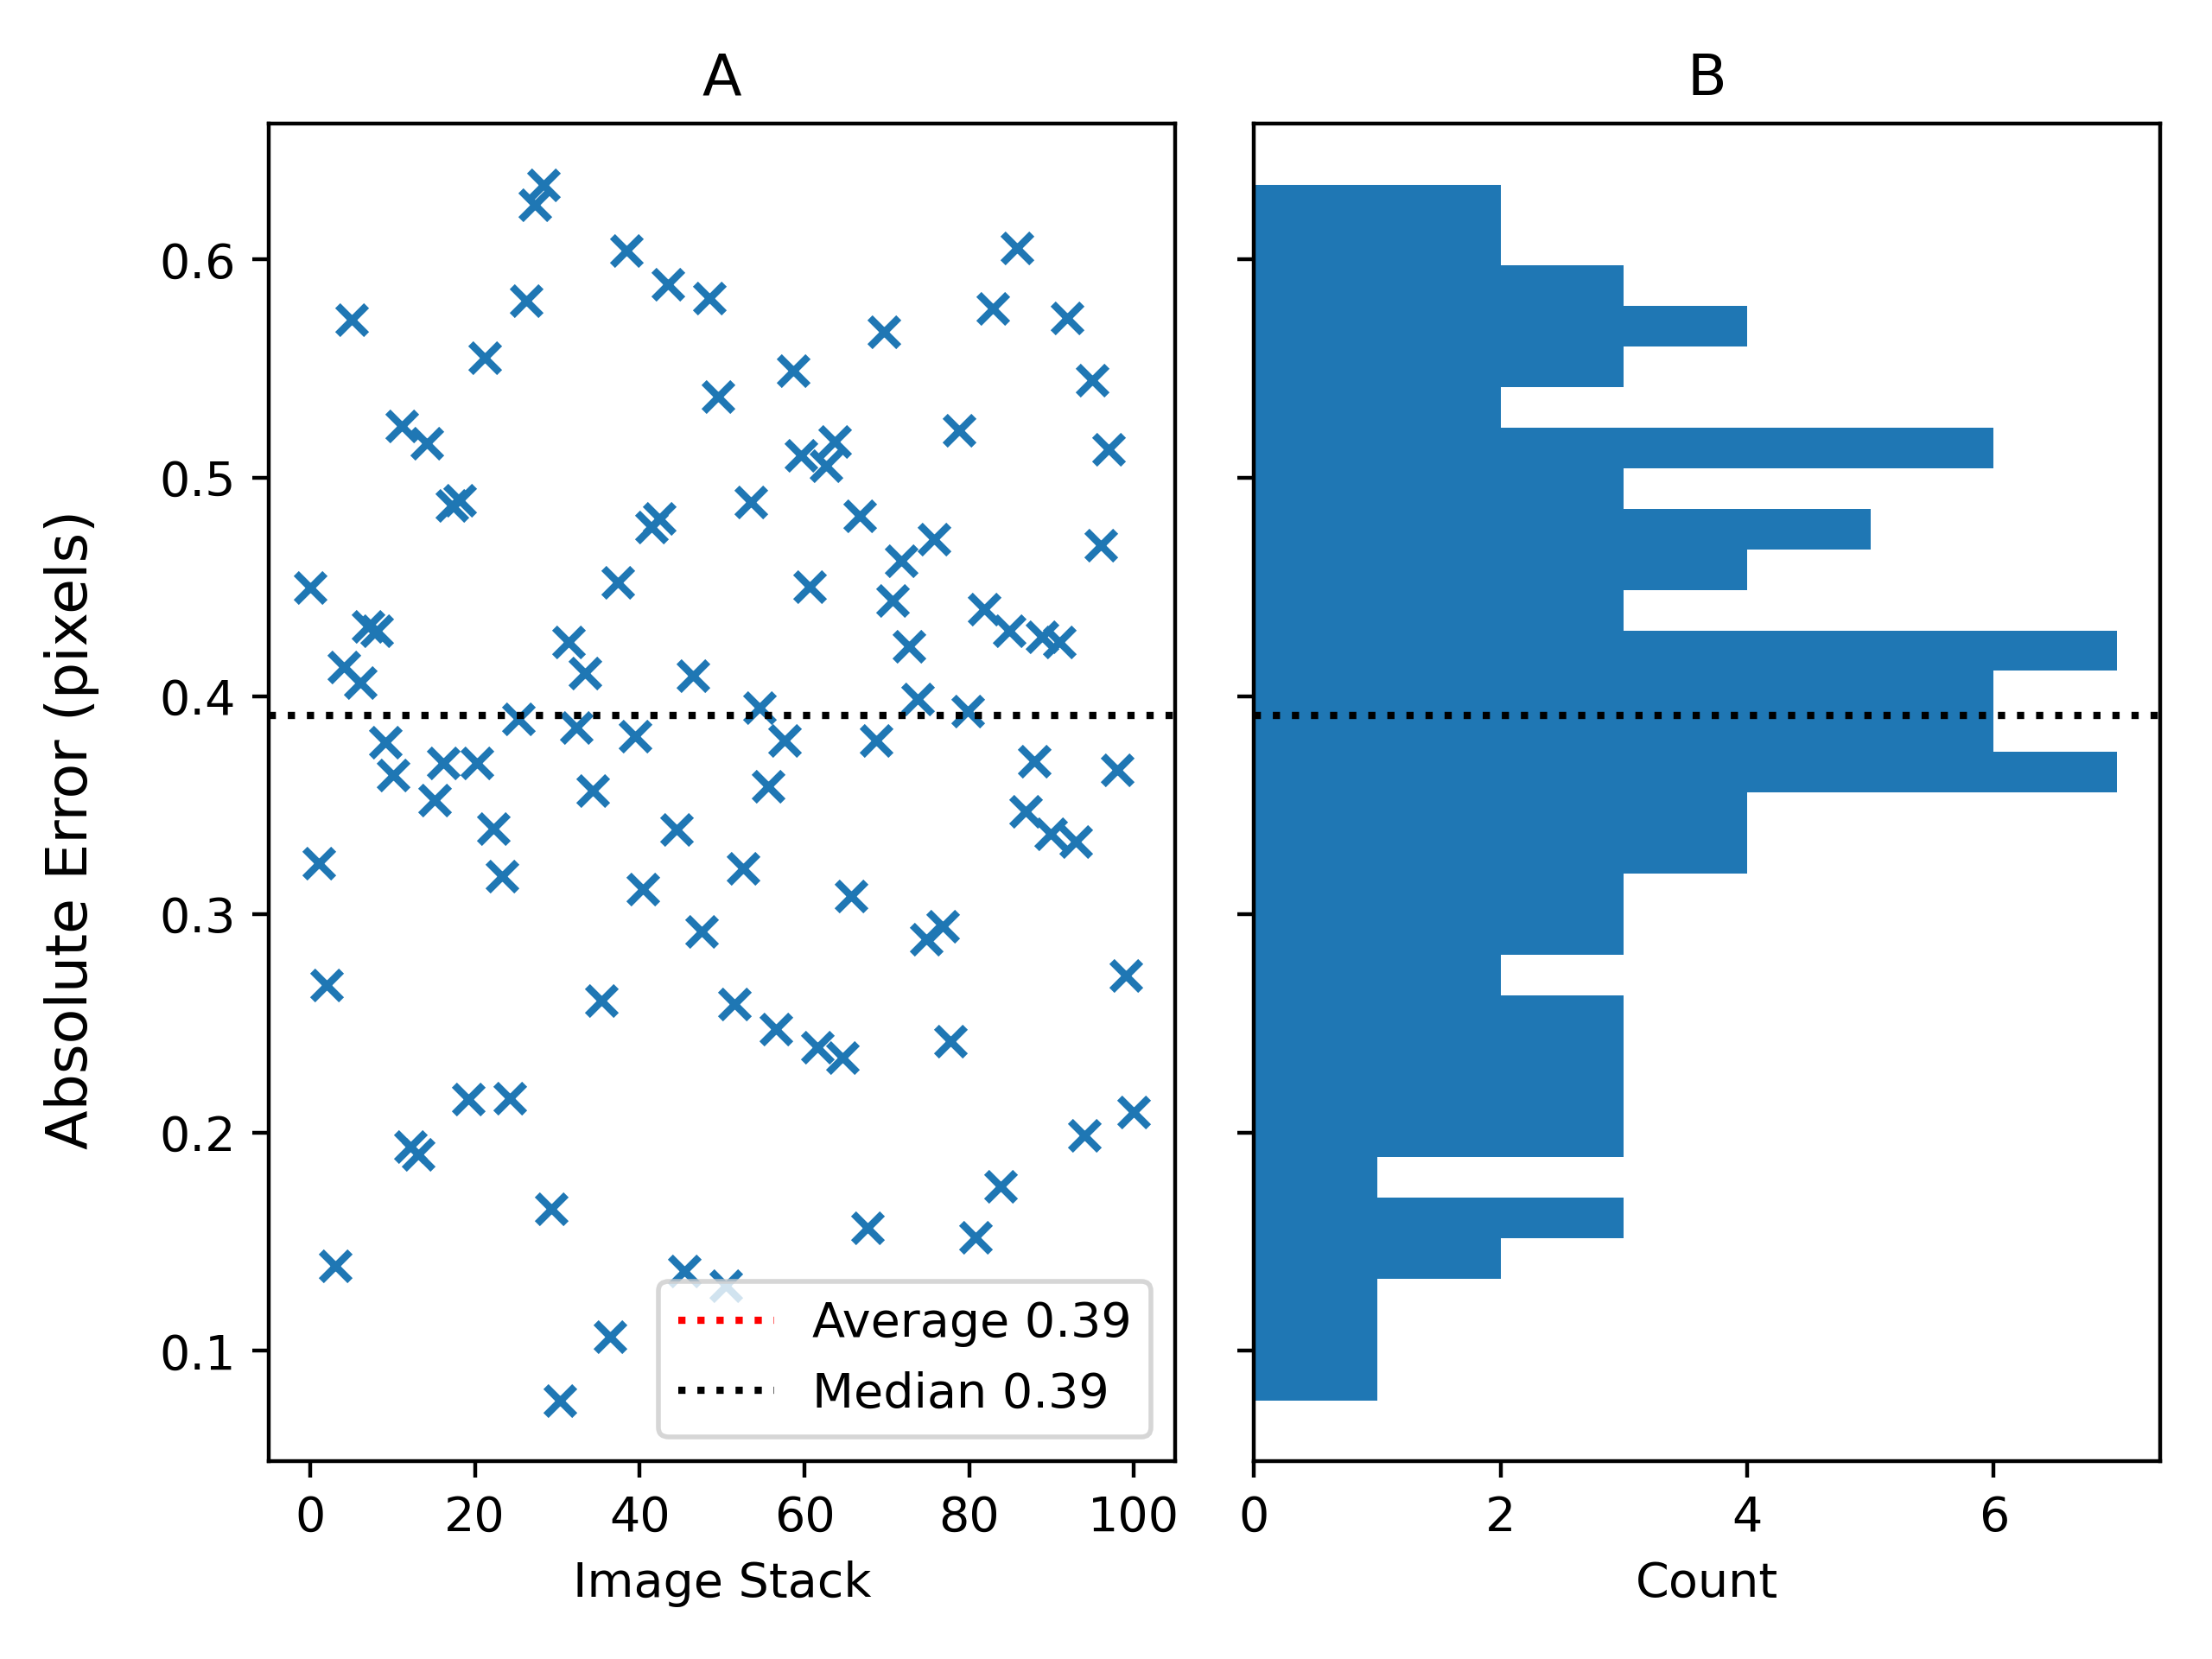
\includegraphics[width=0.6\textwidth]{project_pics/single_histo.png}
    \end{center}
    \caption{A: Absolute error from the ground-truth for R1.00, B: A histogram of errors from graph A}
    \label{fig:single_histo}
  \end{figure}
    
    

\section{Results and analysis} % (fold)
\label{sec:Results}

  \subsection{Centroiding} % (fold)
  \label{sub:Centroiding_results}

  For the centroiding method box sizes of 3, 5, 7 and 11 were used in the production 
  of the histograms pertaining to the absolute error, this was done for the noisy data as 
  well. The rest of the data not presented in the main body of text is available in the appendix 
  section (\ref{sec:appendix}). In all figures for centroiding, all of the combined histograms had 
  taken $\approx 1.4\cdot 10^{-4}$ seconds for all radii and all 100 images in the TIFF stack. This means per 
  spot the time taken to calculate and answer was $\approx 2\cdot 10^{-7}$ seconds

  The results of the centroiding algorithm in figure \ref{fig:box_3} show a fairly poor 
  level of accuracy, ranging from a $0\rightarrow 1.5$ pixel error approximately. This lack of accuracy 
  is especially pronounced the larger the radii of spot, the reason for this increasing 
  error is due to the spots being larger in the same sized 50x50 images. The radii of the 
  airy disk that was used to generate the spots is 'physically' larger than the box size 
  that the centroiding is using. This holds true for the radii that are larger than R1.5 
  as the box size's diameter, as well as the diameter of the airy disk, is 3 pixels. The further 
  increase of inaccuracy seen in figure \ref{fig:box_3} R4.00, R5.66 and R8.00 is due to the 
  3x3 box being placed roughly where the centre of the spot already is, then the algorithm is 
  ran which in essence takes the average of the intensities. This 3x3 box is not given a reasonable 
  range of intensities to average over thus the method will be less likely to give the correct answer,
  this instead gives a range of answers from $0\rightarrow 1.5$ pixels approximately as if the 
  local maximum finder roughly gives an answer the centroiding algorithm will only give and answer 
  that is 1.5 pixels off of that guess. Since in this perfect data that only has one spot per image, the 
  local maximum finder will predict where the spot is to a single pixel of accuracy thus the maximum 
  error seen should indeed be fractionally larger than 1.5 pixels as observed.

  \begin{figure}[h]
    \begin{center}
      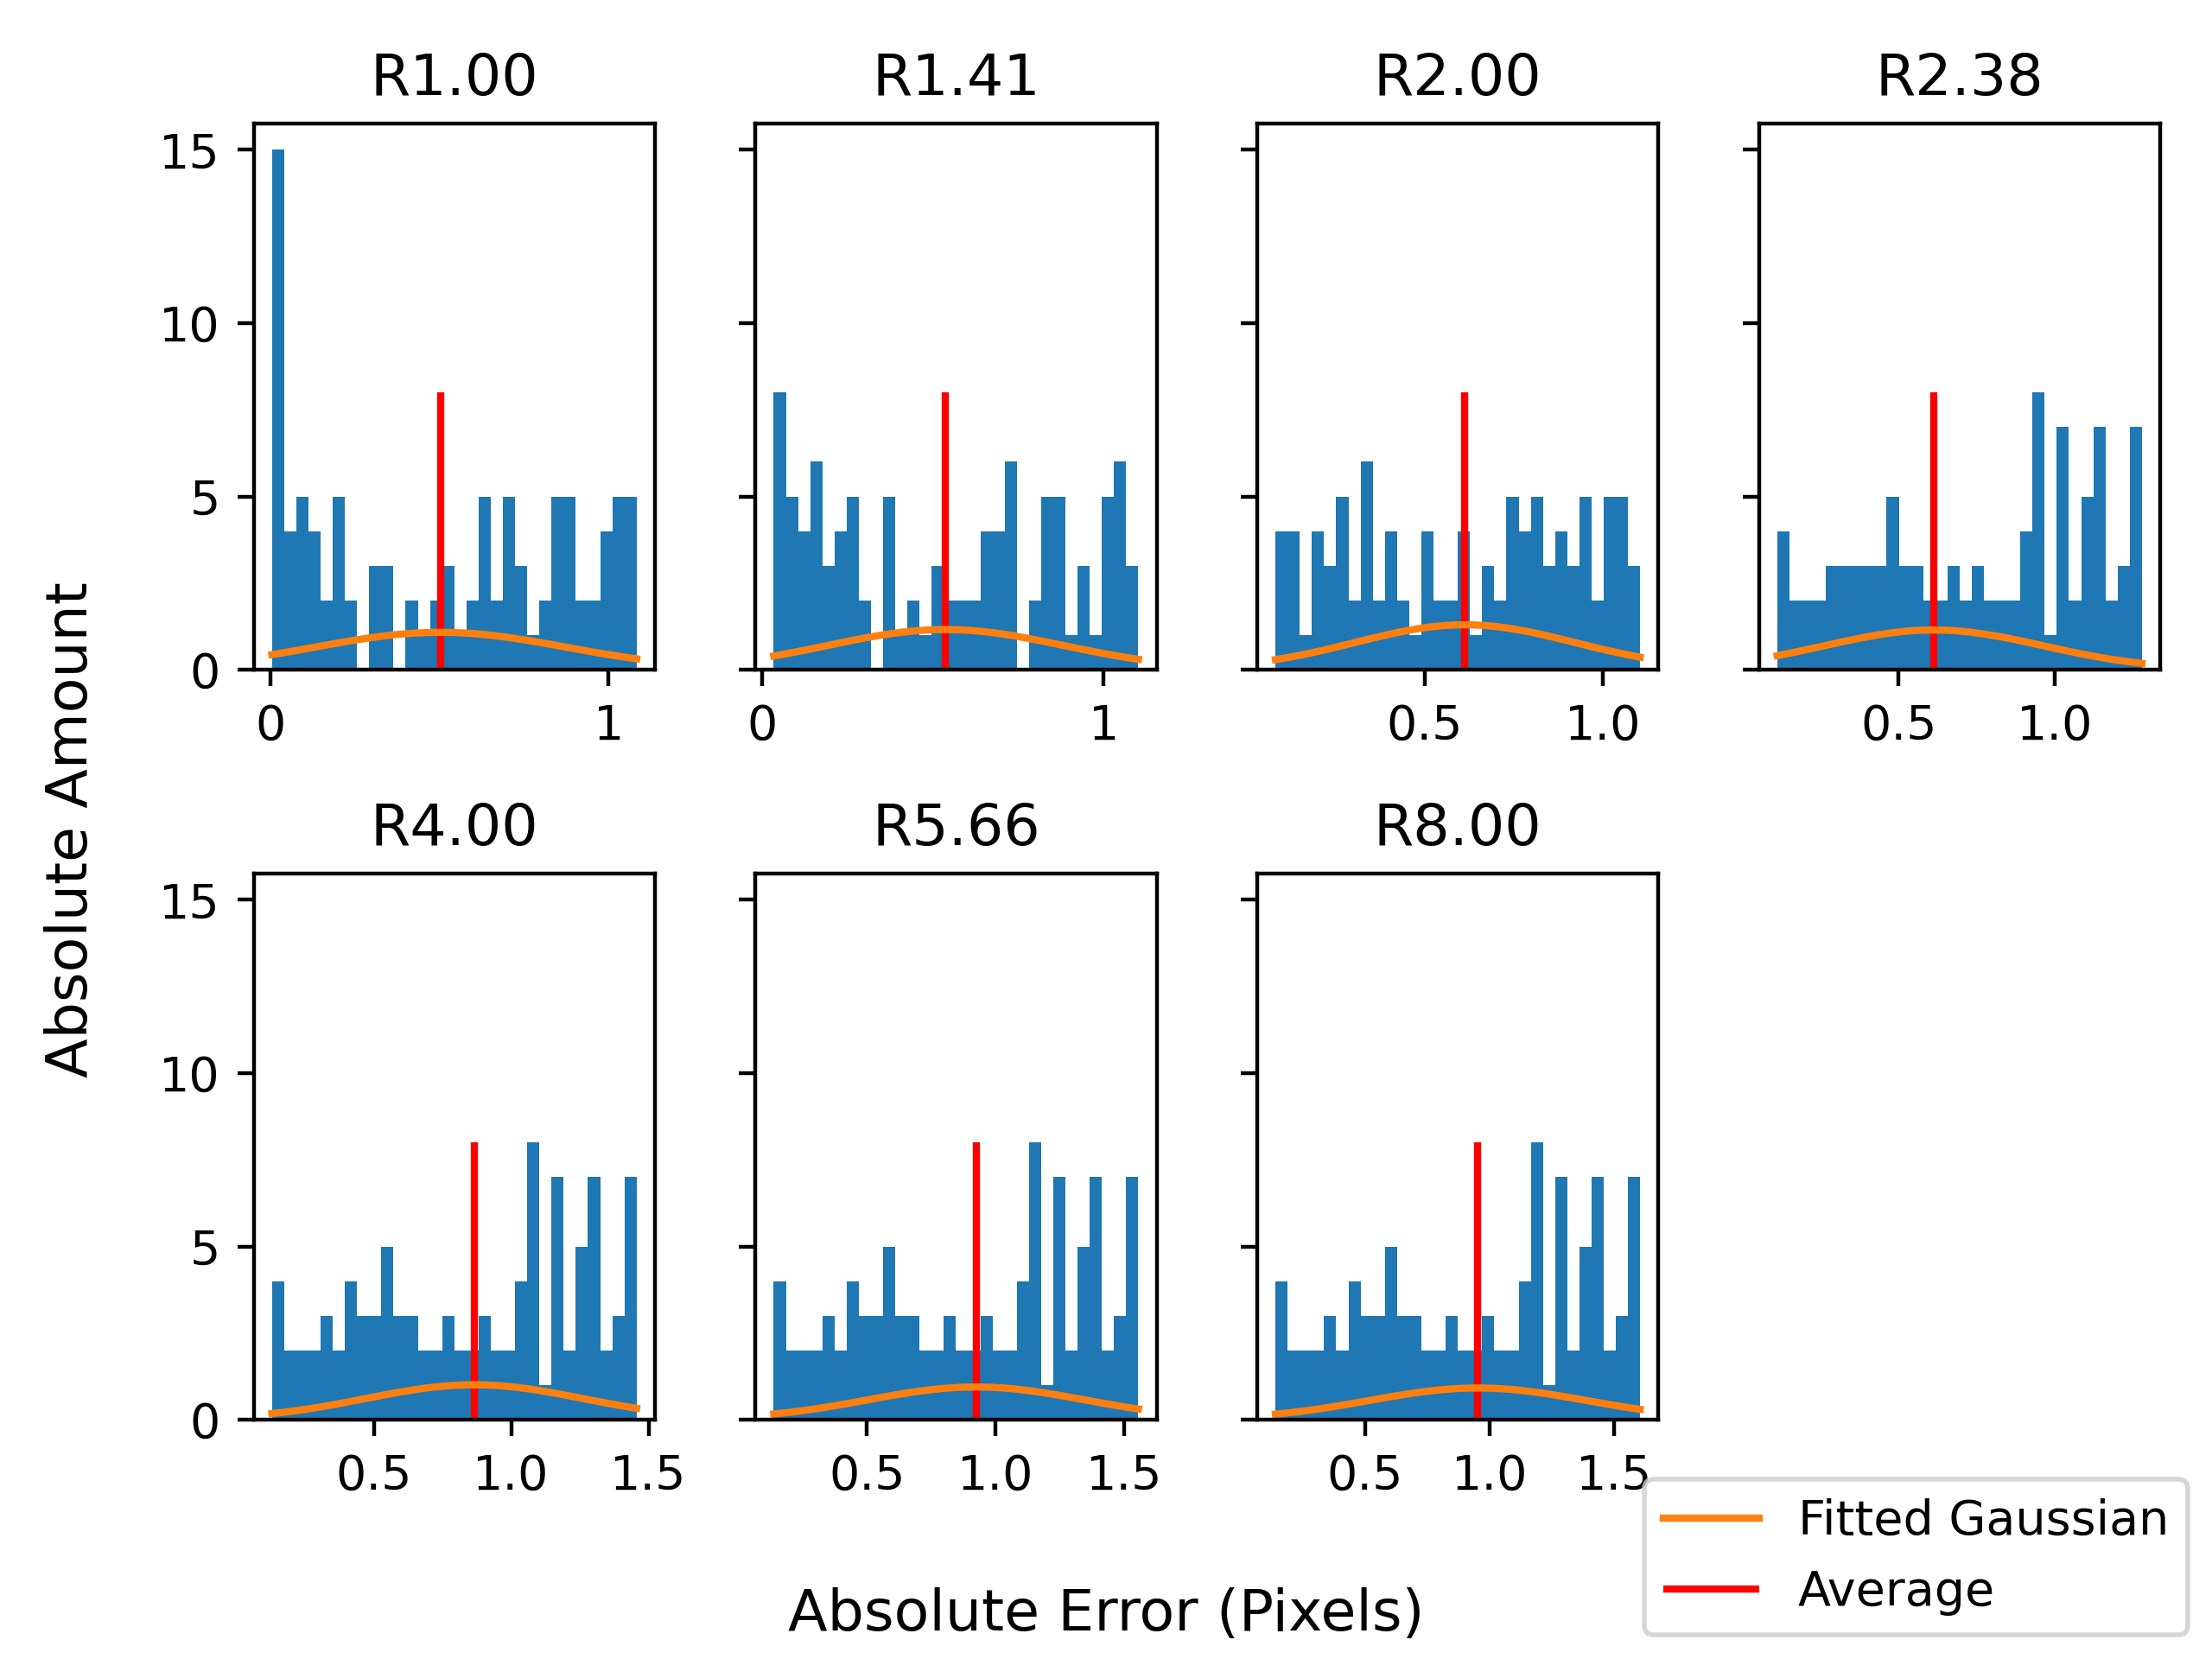
\includegraphics[width=0.6\textwidth]{project_pics/distro_centriod_3.png}
    \end{center}
    \caption{Histograms of the absolute error from each radii with a box size of 3x3 pixels. Completed in $\approx 1.4\cdot 10^{-4}$s}
    \label{fig:box_3}
  \end{figure}

  In figure \ref{fig:box_3_noise} noisy spot data was provided to test out the algorithms on, 
  these spot were the same as before but with read noise at 1 electron, average photon number 
  per spot at 2000 and dark current at 0.1 electron per pixel and cg? Also the number of radii 
  were reduced, R1.00 and R1.41 were removed. These noise values were chosen 
  to replicate real world noise levels in order to test all algorithms in isolation from any other 
  variables so that the spot finding methods could be objectively observed. 

  The noisy data for the 3x3 centroid box size did not have a pronounced impact on average 
  accuracy per radii. This again is due to the size of the box being small relative to the 
  size of the spots, thus mostly not allowing the noise to play a part in the calculation of the 
  centre of the spot. One difference that the noisy data does seem to show is that it gives a more 
  even spread of answers around it's average, this suggests that although the noisy data 
  is not changing the average it is having an effect on the centroiding algorithm. The limiting factor 
  in this case is the box size in which the algorithm is interested in.

  \begin{figure}[h]
    \begin{center}
      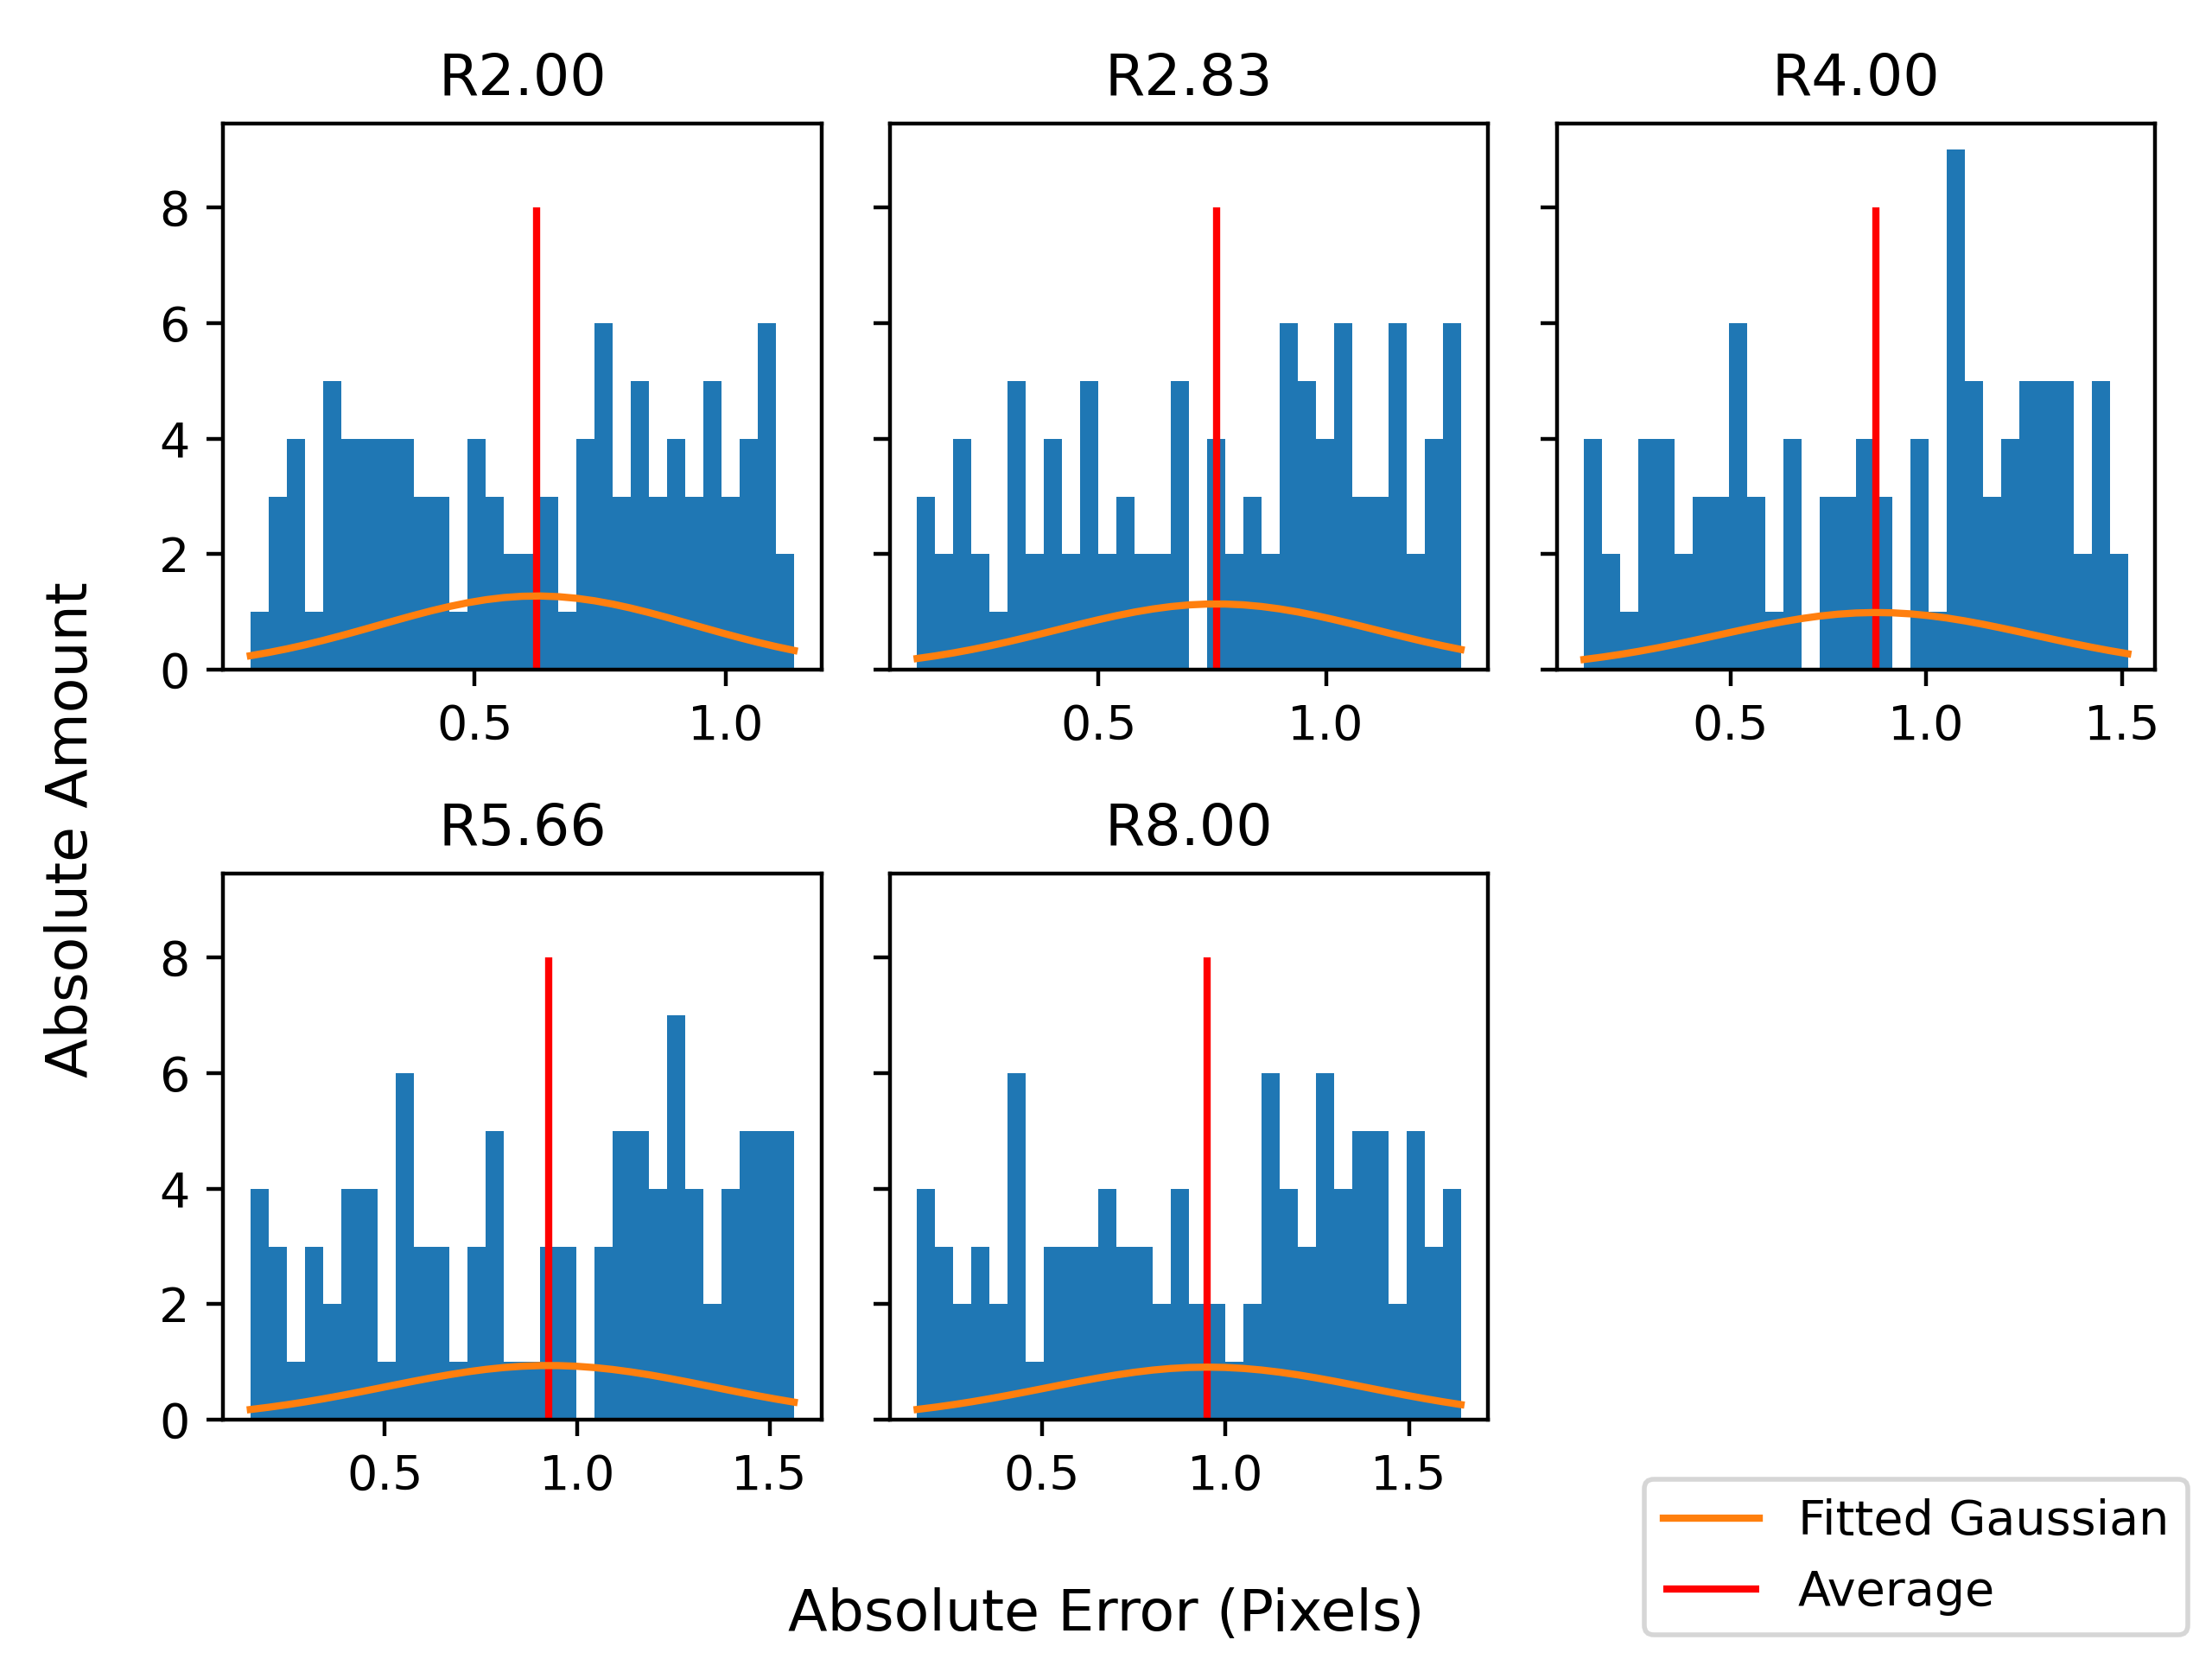
\includegraphics[width=0.6\textwidth]{project_pics/noise_cen_scatter_3.png}
    \end{center}
    \caption{Histograms of the absolute error from each radii with a box size of 3x3 pixels, with noise.}
    \label{fig:box_3_noise}
  \end{figure}
  


  In figure \ref{fig:box_11} the box size used was 11x11, this increases the sub-pixel localisation 
  drastically compared to figure \ref{fig:box_3}. The spread of all answers is smaller using 11x11 instead of using 3x3
  boxes, the spread also changes with radii sequentially getting larger along with the average. 
  This is due to the larger box size being able to fit 
  more pixels in to average over effectively, this is clearly evident in the R5.66 and R8.00 histogram as there is a 
  significant jump in inaccuracy as the radii is still larger than the radii of the box. 

  \begin{figure}[H]
    \begin{center}
      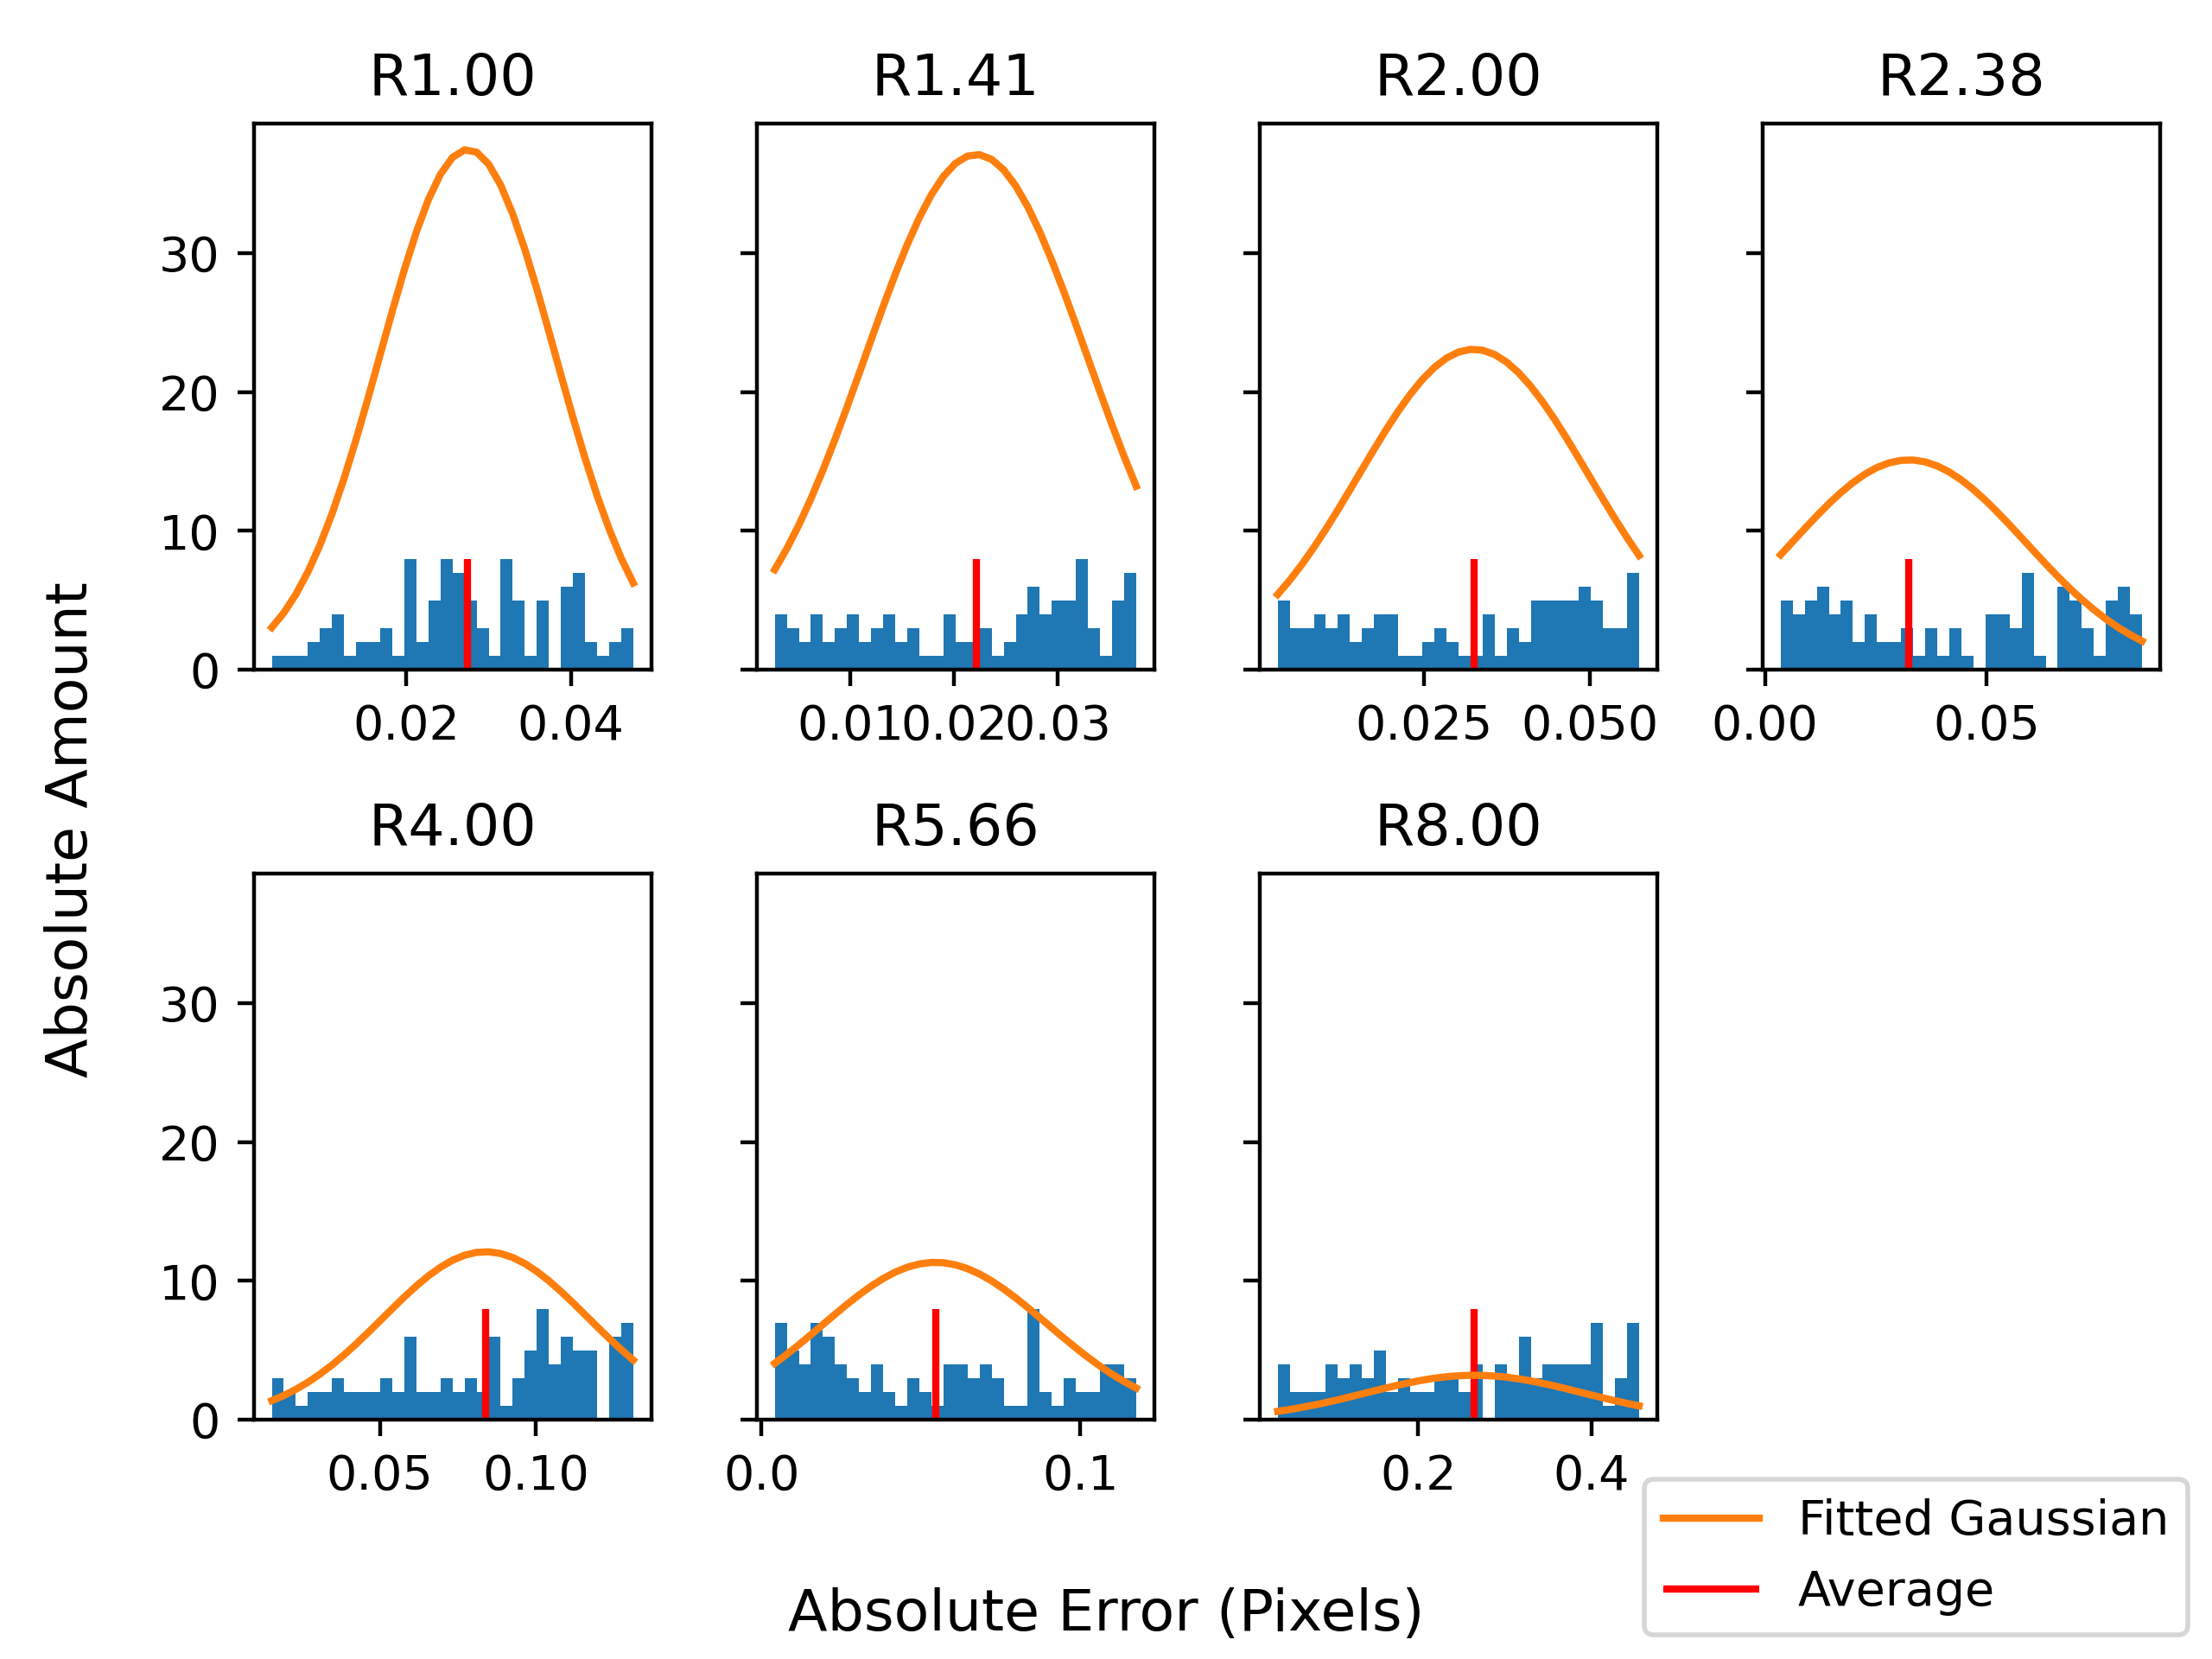
\includegraphics[width=0.6\textwidth]{project_pics/distro_centriod_11.png}
    \end{center}
    \caption{Histograms of the absolute error from each radii with a box size of 11x11 pixels.}
    \label{fig:box_11}
  \end{figure}
  
  In figure \ref{fig:box_11_noise} when centroiding was used on the noisy data with an 11x11 box size, 
  on average the accuracy decreased as expected and gave a similar average error for each radii apart from R8.00. 
  Again this will be due to the fact that the R8.00 spot will not fit into the box size being calculated 
  but also in relation to the spot, as the size of the spot increases so to does the noise in the images 
  provided.


  \begin{figure}[H]
    \begin{center}
      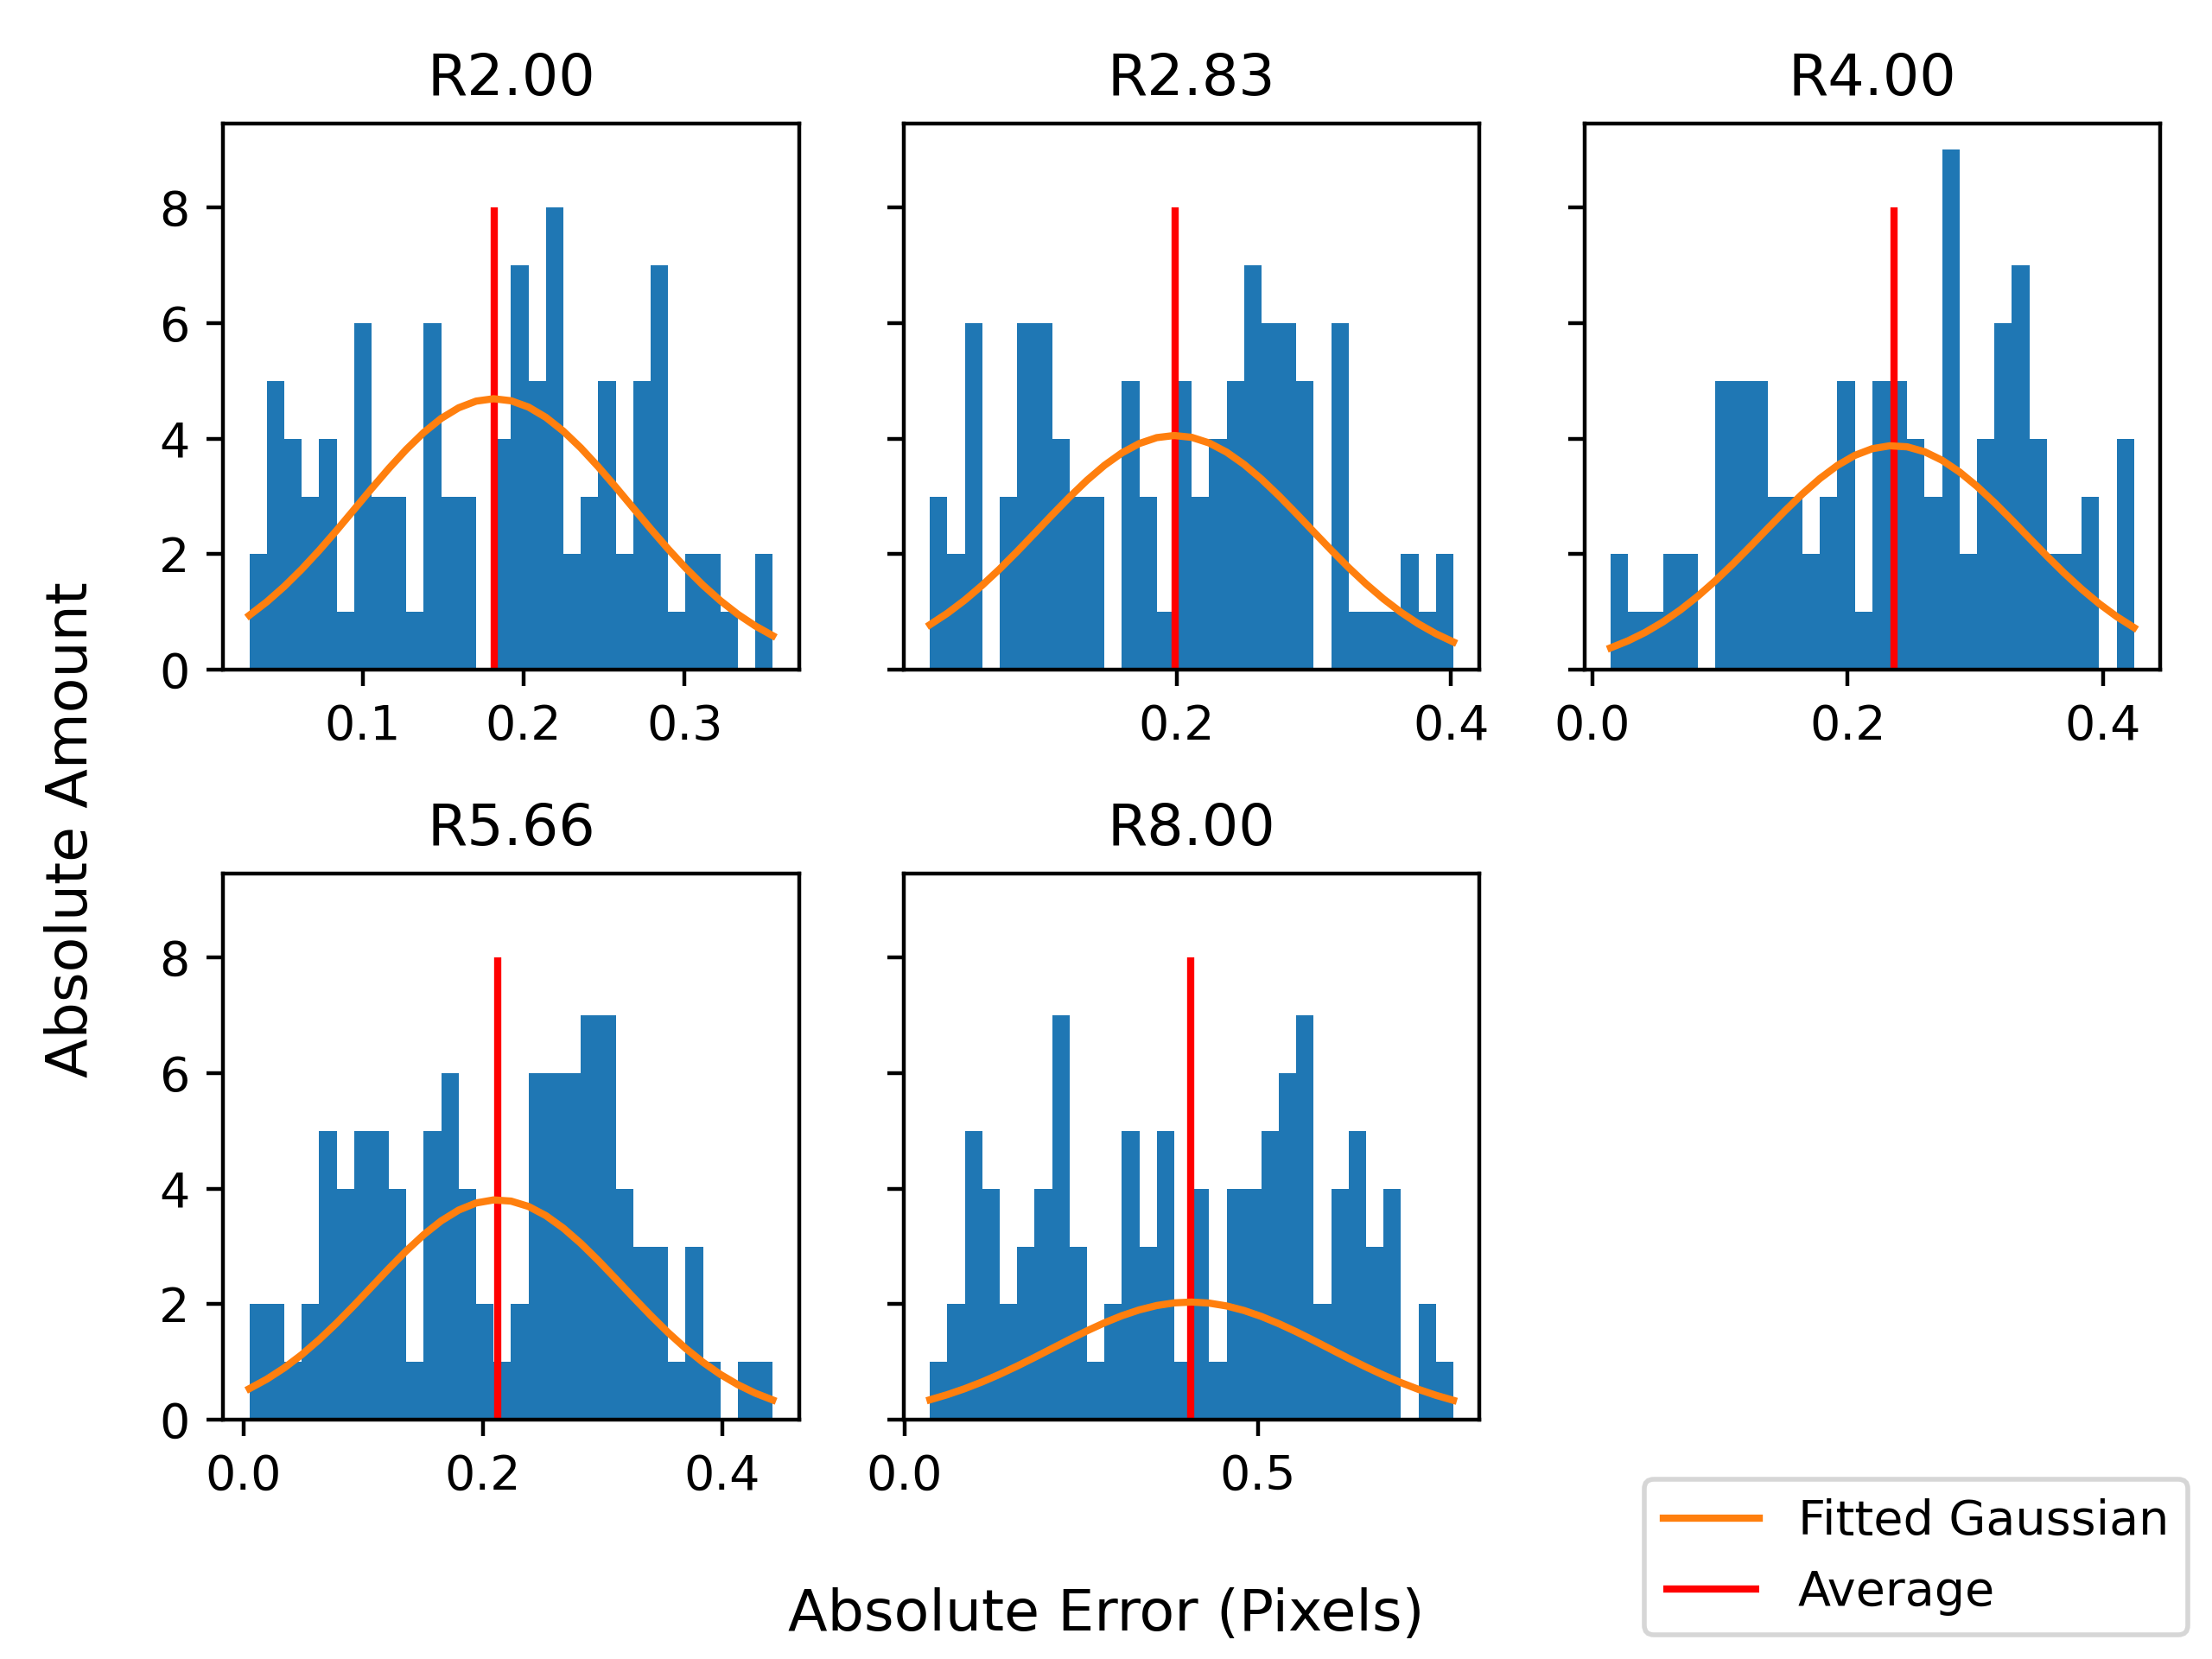
\includegraphics[width=0.6\textwidth]{project_pics/noise_cen_scatter_11.png}
    \end{center}
    \caption{Histograms of the absolute error from each radii with a box size of 11x11 pixels, with noise.}
    \label{fig:box_11_noise}
  \end{figure}
  
  In figure \ref{fig:box_var_r2} the box size for making the centroiding calculation 
  was varied from 3 to 15 $\textrm{pixels}^2$ in odd increments, this was tested to understand the 
  relationship between box size and accuracy. In general the larger the box size the more accuracy 
  gained this was expected especially for the perfect data as there was only one spot per image, 
  although this would be impractical for real data as spot are more than likely to be closer than 
  $\approx 15$ pixels. 

  \begin{figure}[H]
    \begin{center}
      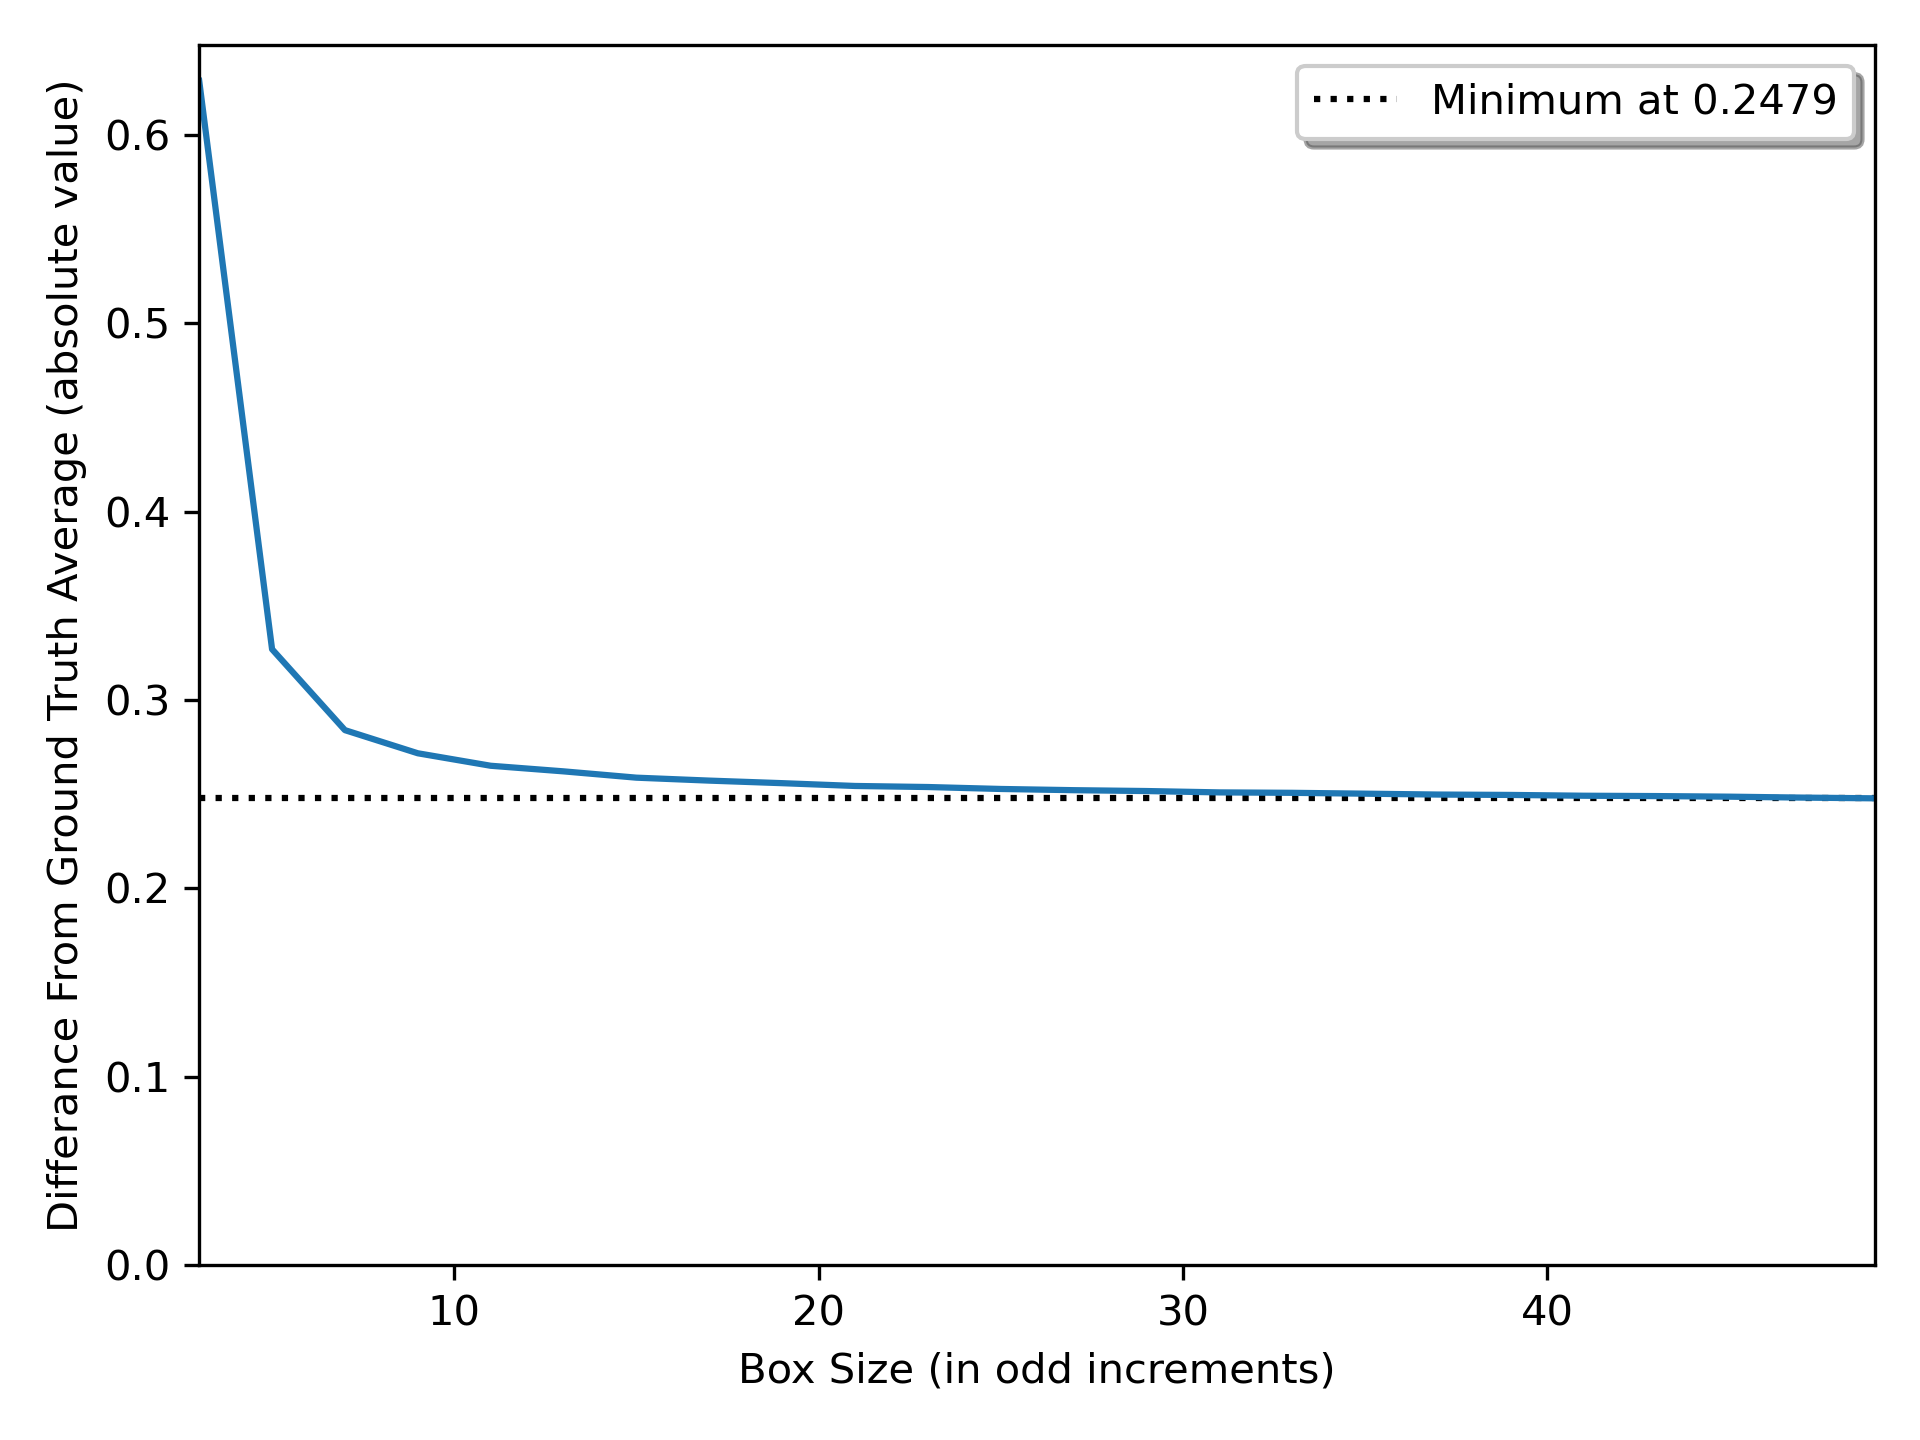
\includegraphics[width=0.5\textwidth]{project_pics/box_size_var_r2.png}
    \end{center}
    \caption{Showing the accuracy of centroiding Vs the box size chosen, for a radii or R2.00.}
    \label{fig:box_var_r2}
  \end{figure}

  Figure \ref{fig:noise_box_r2}, similar to figure \ref{fig:box_var_r2}, shows the accuracy of the 
  centroid method against the varying box size, but on a set of noisy data. Here it can be seen that 
  for a period of box size increases the accuracy also increases, then it minimises and then decreases indefinitely.
  This specific box size minimises the error at $\approx 9$ pixels due to the radii being R2.00, 
  as each spot size will be optimised at a certain box size that's more than double it's radii. For noisy spots 
  this optimisation can not be too large as the centroiding algorithm is known for being highly sensitive. \cite{delabie2014accurate}


  \begin{figure}[H]
    \begin{center}
      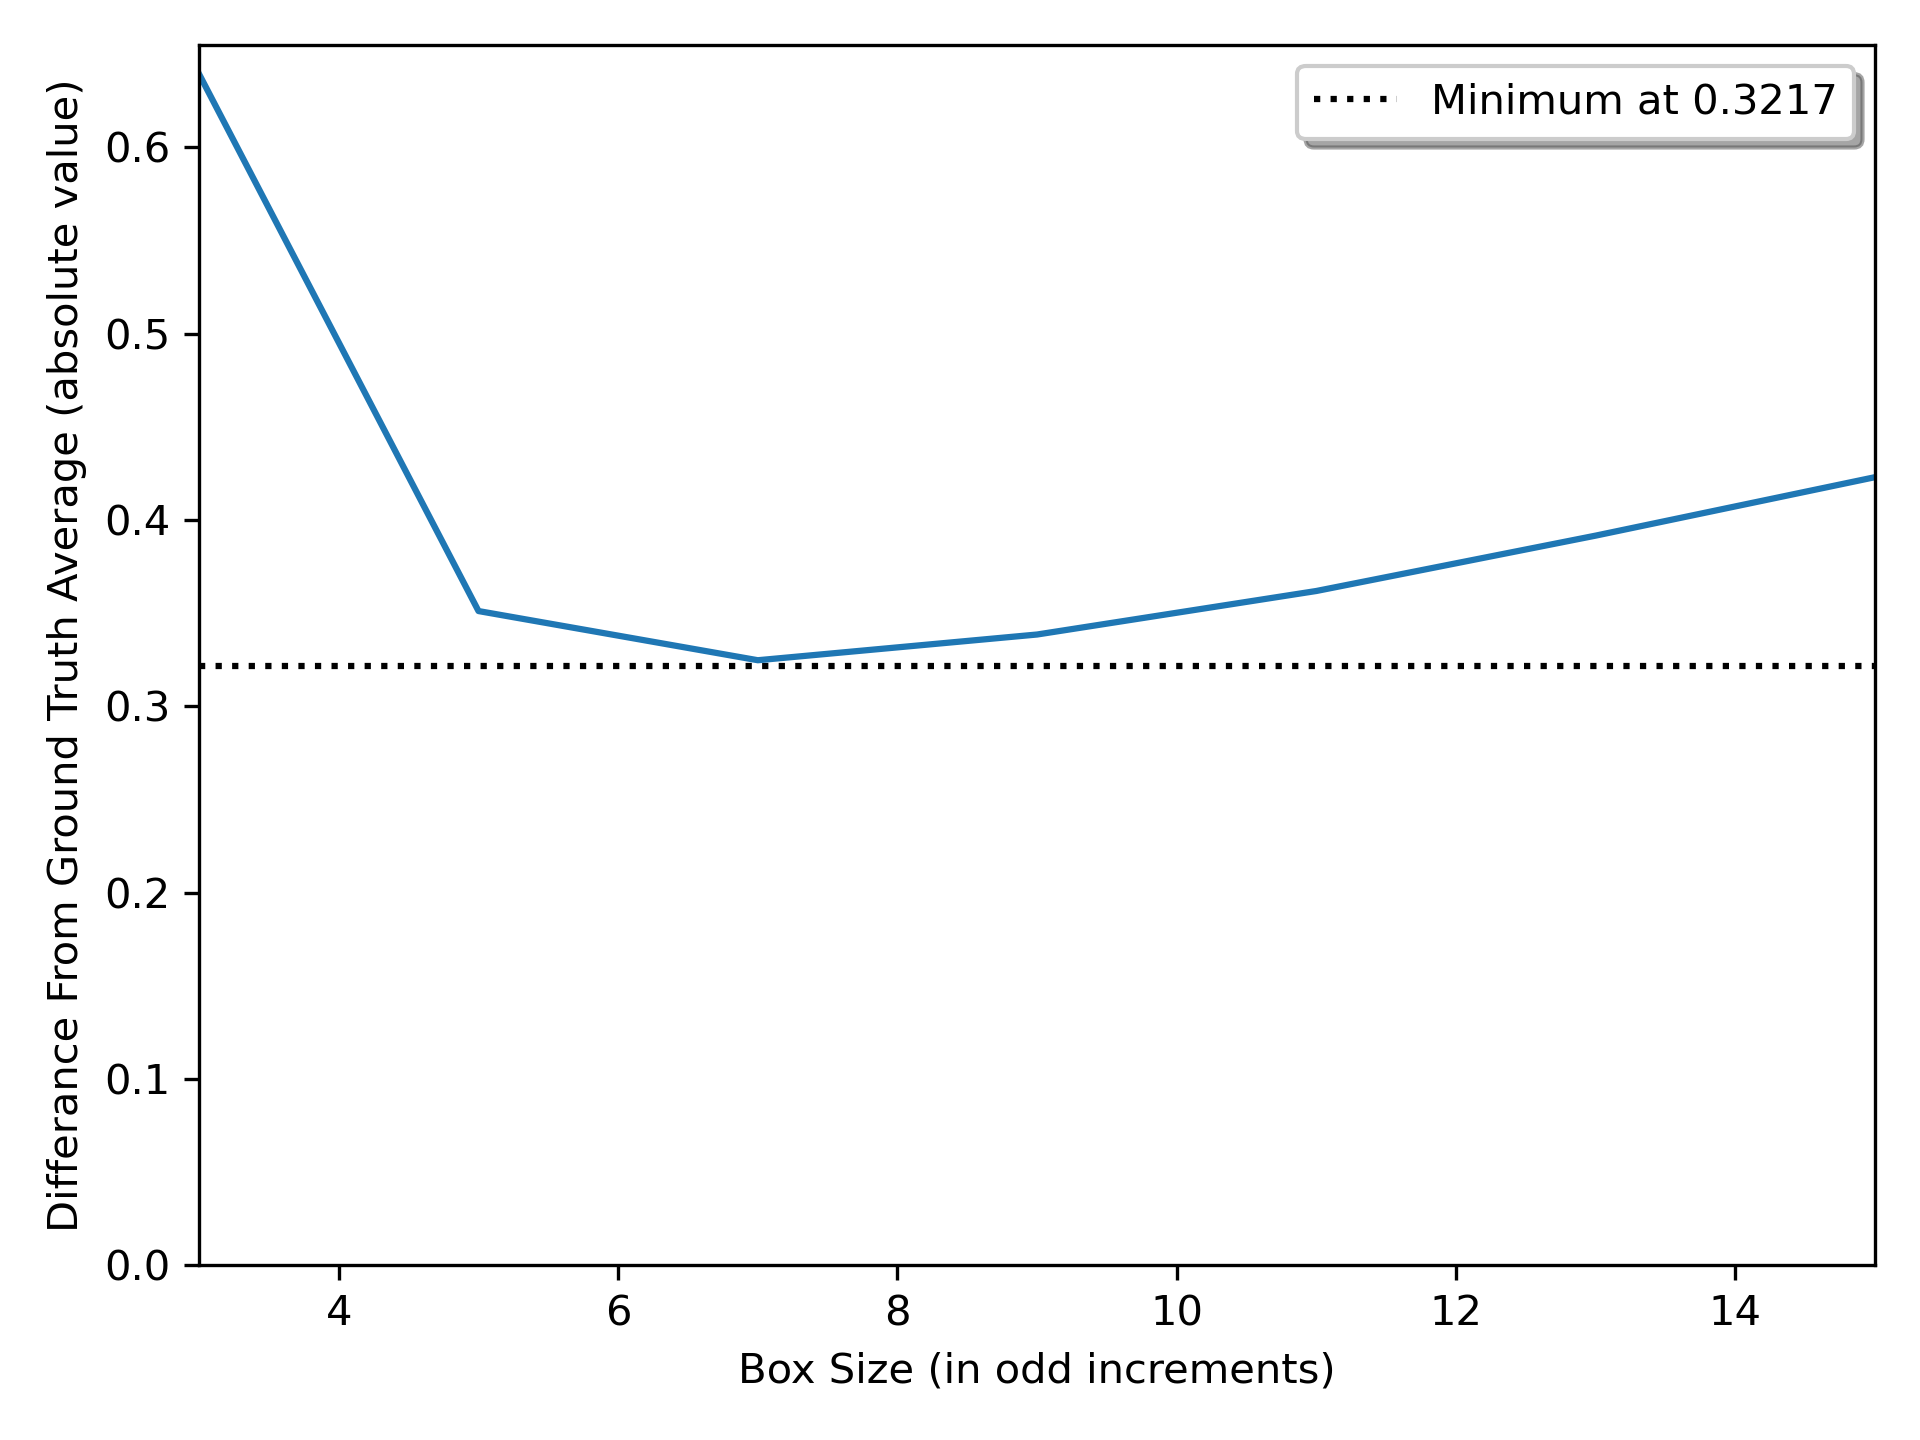
\includegraphics[width=0.5\textwidth]{project_pics/box_size_var_r2_noise.png}
    \end{center}
    \caption{Showing the accuracy of centroiding Vs the box size chosen, for a radii or R2.00 and with noise}
    \label{fig:noise_box_r2}
  \end{figure}


  \subsection{Triangle Fitting} % (fold)
  \label{sub:Triangle Fitting}

  In figure \ref{fig:single_test} it can be seen that while using simulated data of radii R1.00, the mean accuracy of the 
  localisation is $\approx 0.4$ of a pixel whilst being executed in $\approx 0.34$ seconds. This time to complete a computation 
  was the same for all individual radii, for all the data the time taken was $\approx 2.4$ seconds. This means an 
  average time to calculate a spot using the triangle method takes $\approx 3.3\cdot 10^{-3}$ seconds.Part C of 
  figure \ref{fig:single_test} has been replicated for all simulated spots given in figure \ref{fig:no_noise_all_r}
  to compare how the change in spot size changes accuracy.
  Figure \ref{fig:distro} shows the histogram results of the triangle fitting method on the perfect simulated data. 
  Compared with the 3x3 centroiding method (figure \ref{fig:box_3}) the average accuracy of this method is better, especially for the 
  larger radii, ranging from a $\approx 1.33\rightarrow 2.6$ times improvement. This comes at a $\approx 16500$ times 
  increase in computational time to produce an answer however. A reason for this apparent increase in accuracy will be 
  because of the fact that the box size is limiting the amount of the image the centroiding method can calculate over.
  If this method is compared with the 11x11 centroiding method (figure \ref{fig:box_11}) then there is a substantial 
  difference in average accuracy, ranging from $\approx 19 \rightarrow 1.25$ times better accuracy for the centroiding 
  method whilst also still having a $\approx 16500$ times computational speed advantage.

  \begin{figure}[H]
    \begin{center}
      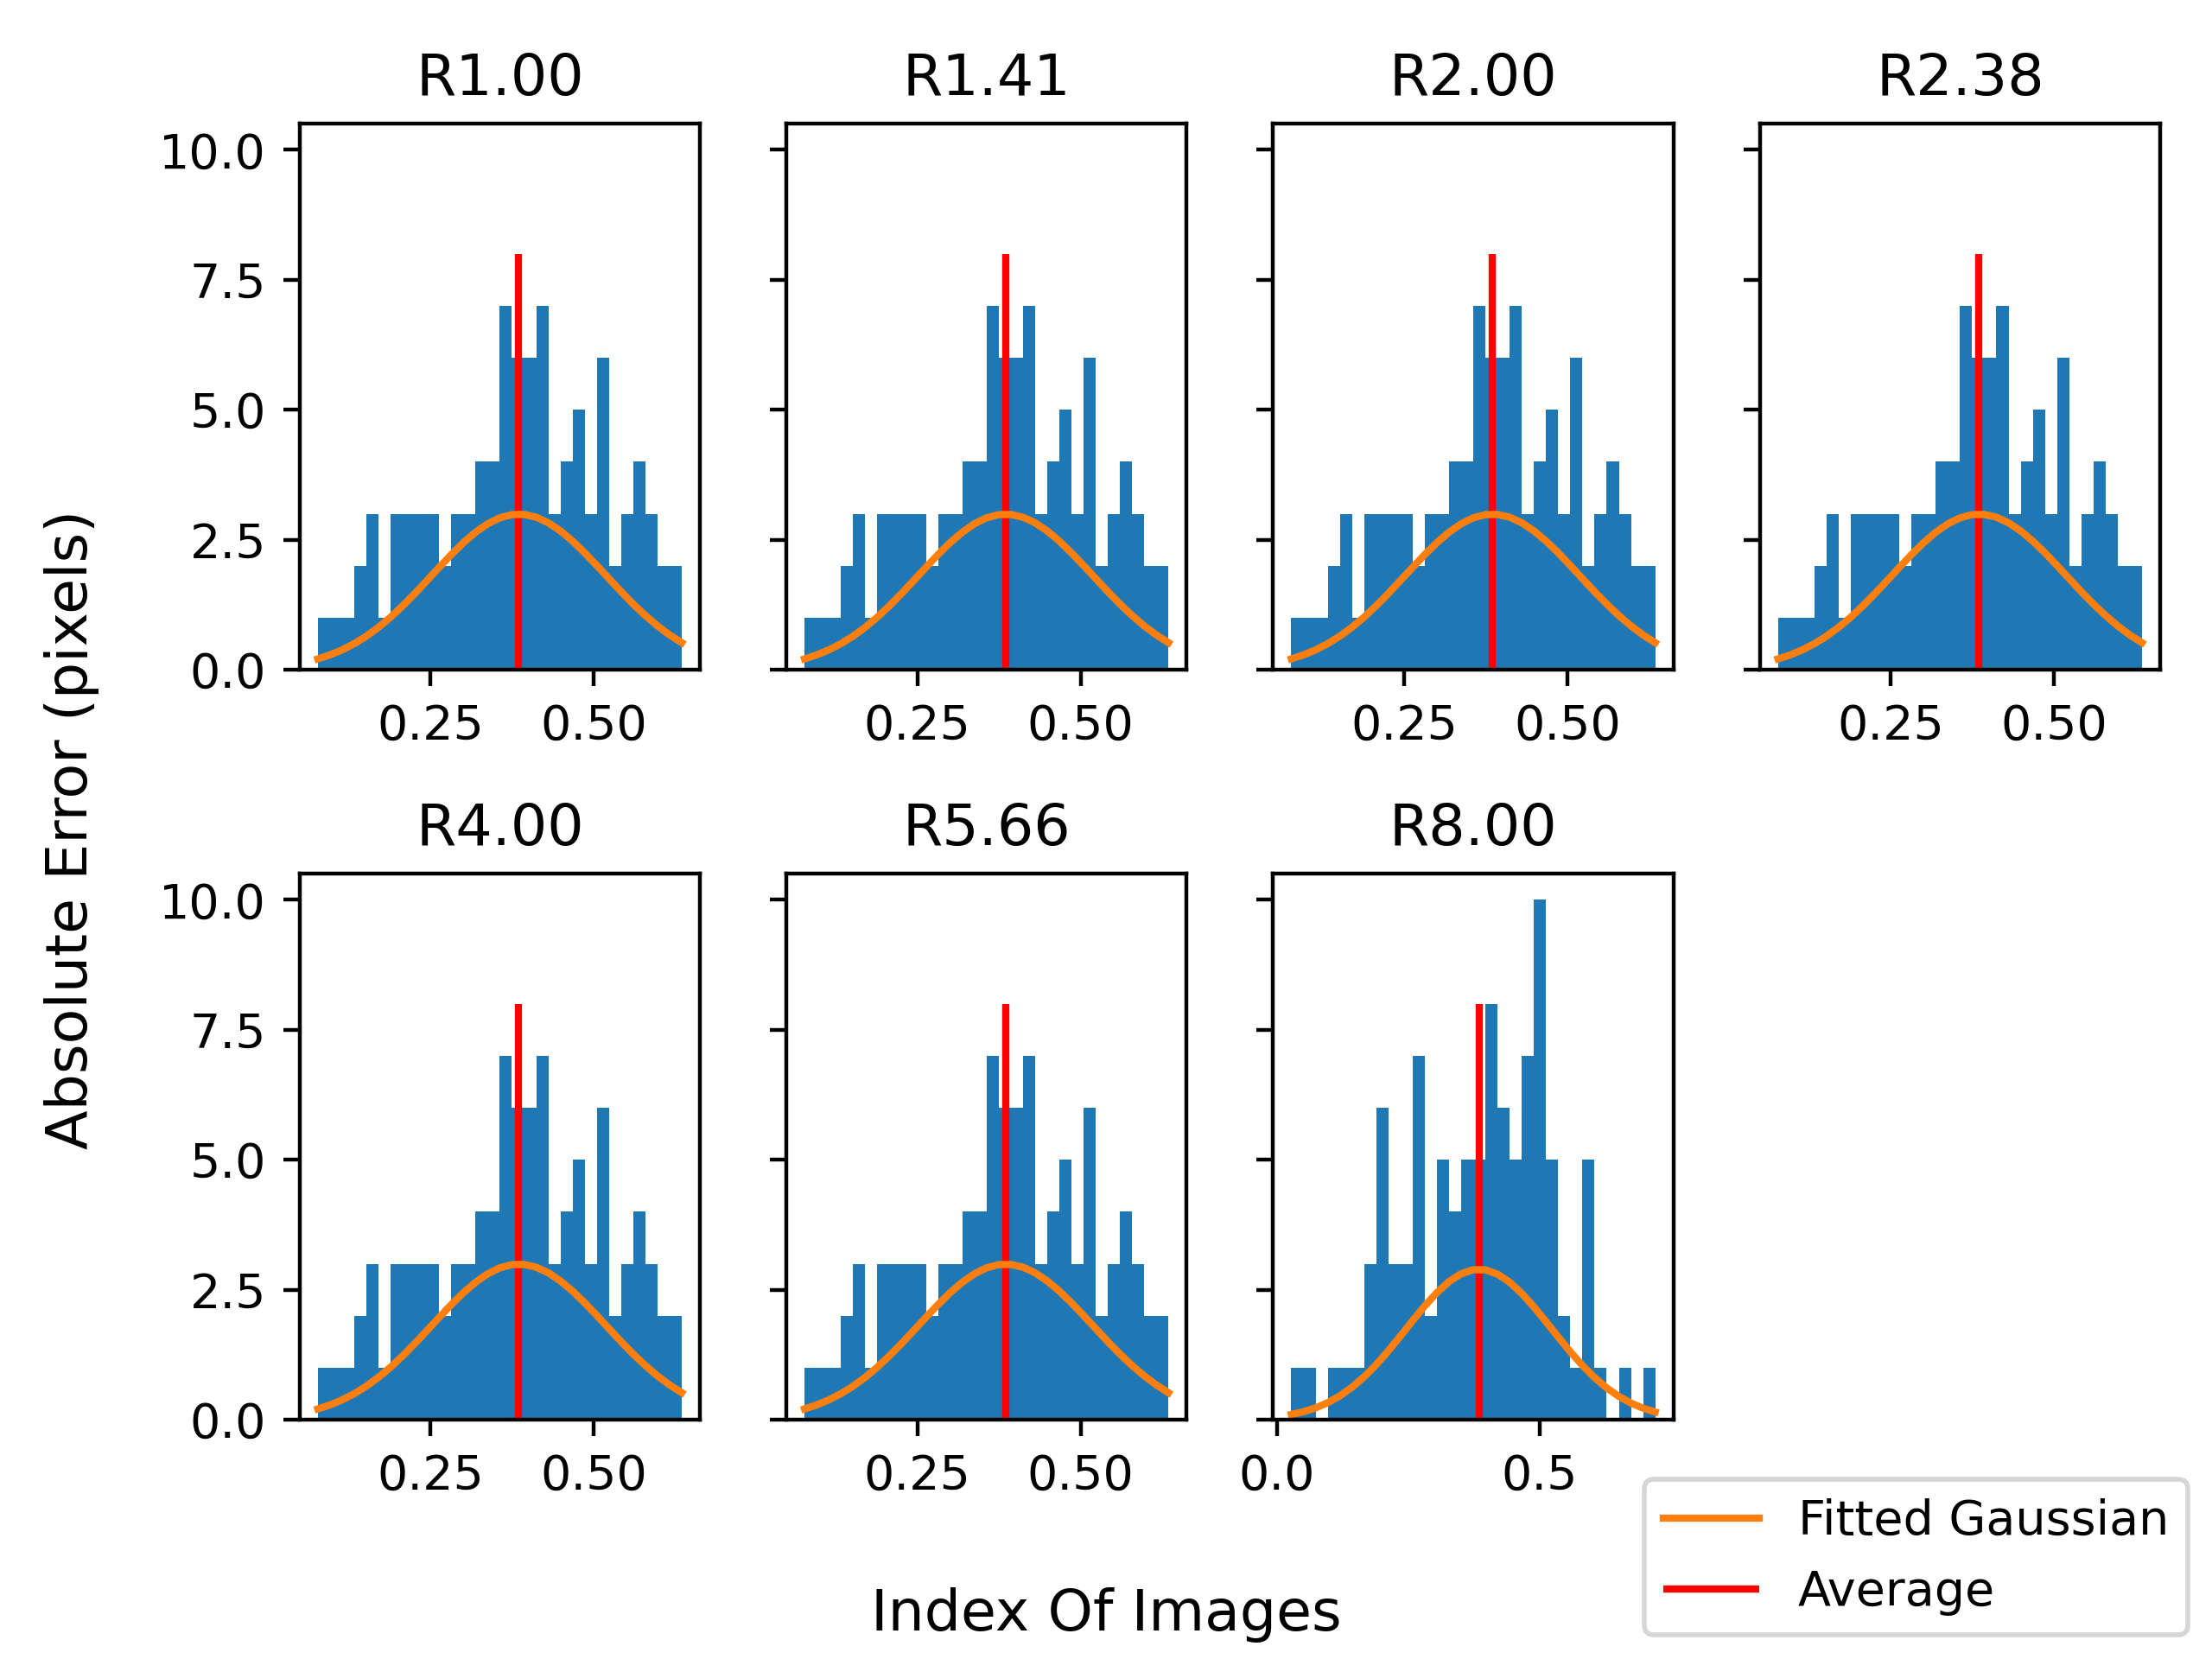
\includegraphics[width=0.7\textwidth]{project_pics/distro.png}
    \end{center}
    \caption{Histograms of the absolute error from each radii}
    \label{fig:distro}
  \end{figure}

  As can be seen in figure \ref{fig:distro_noise}, compared with figure \ref{fig:distro}, the distribution
  of results is shifted towards being less accurate. This is expected as noise adds randomness and 
  variability into the system, giving extra information that does not aid in the process of finding the 
  centre of a spot. If figure \ref{fig:distro_noise} is compared with figure \ref{fig:box_11_noise}, again, 
  it can be seen that the centroiding method achieves better results, ranging from $\approx 1.5\rightarrow 2$
  times more accurate than the triangle method and again being $\approx 16500$ times faster.

  \begin{figure}[H]
    \begin{center}
      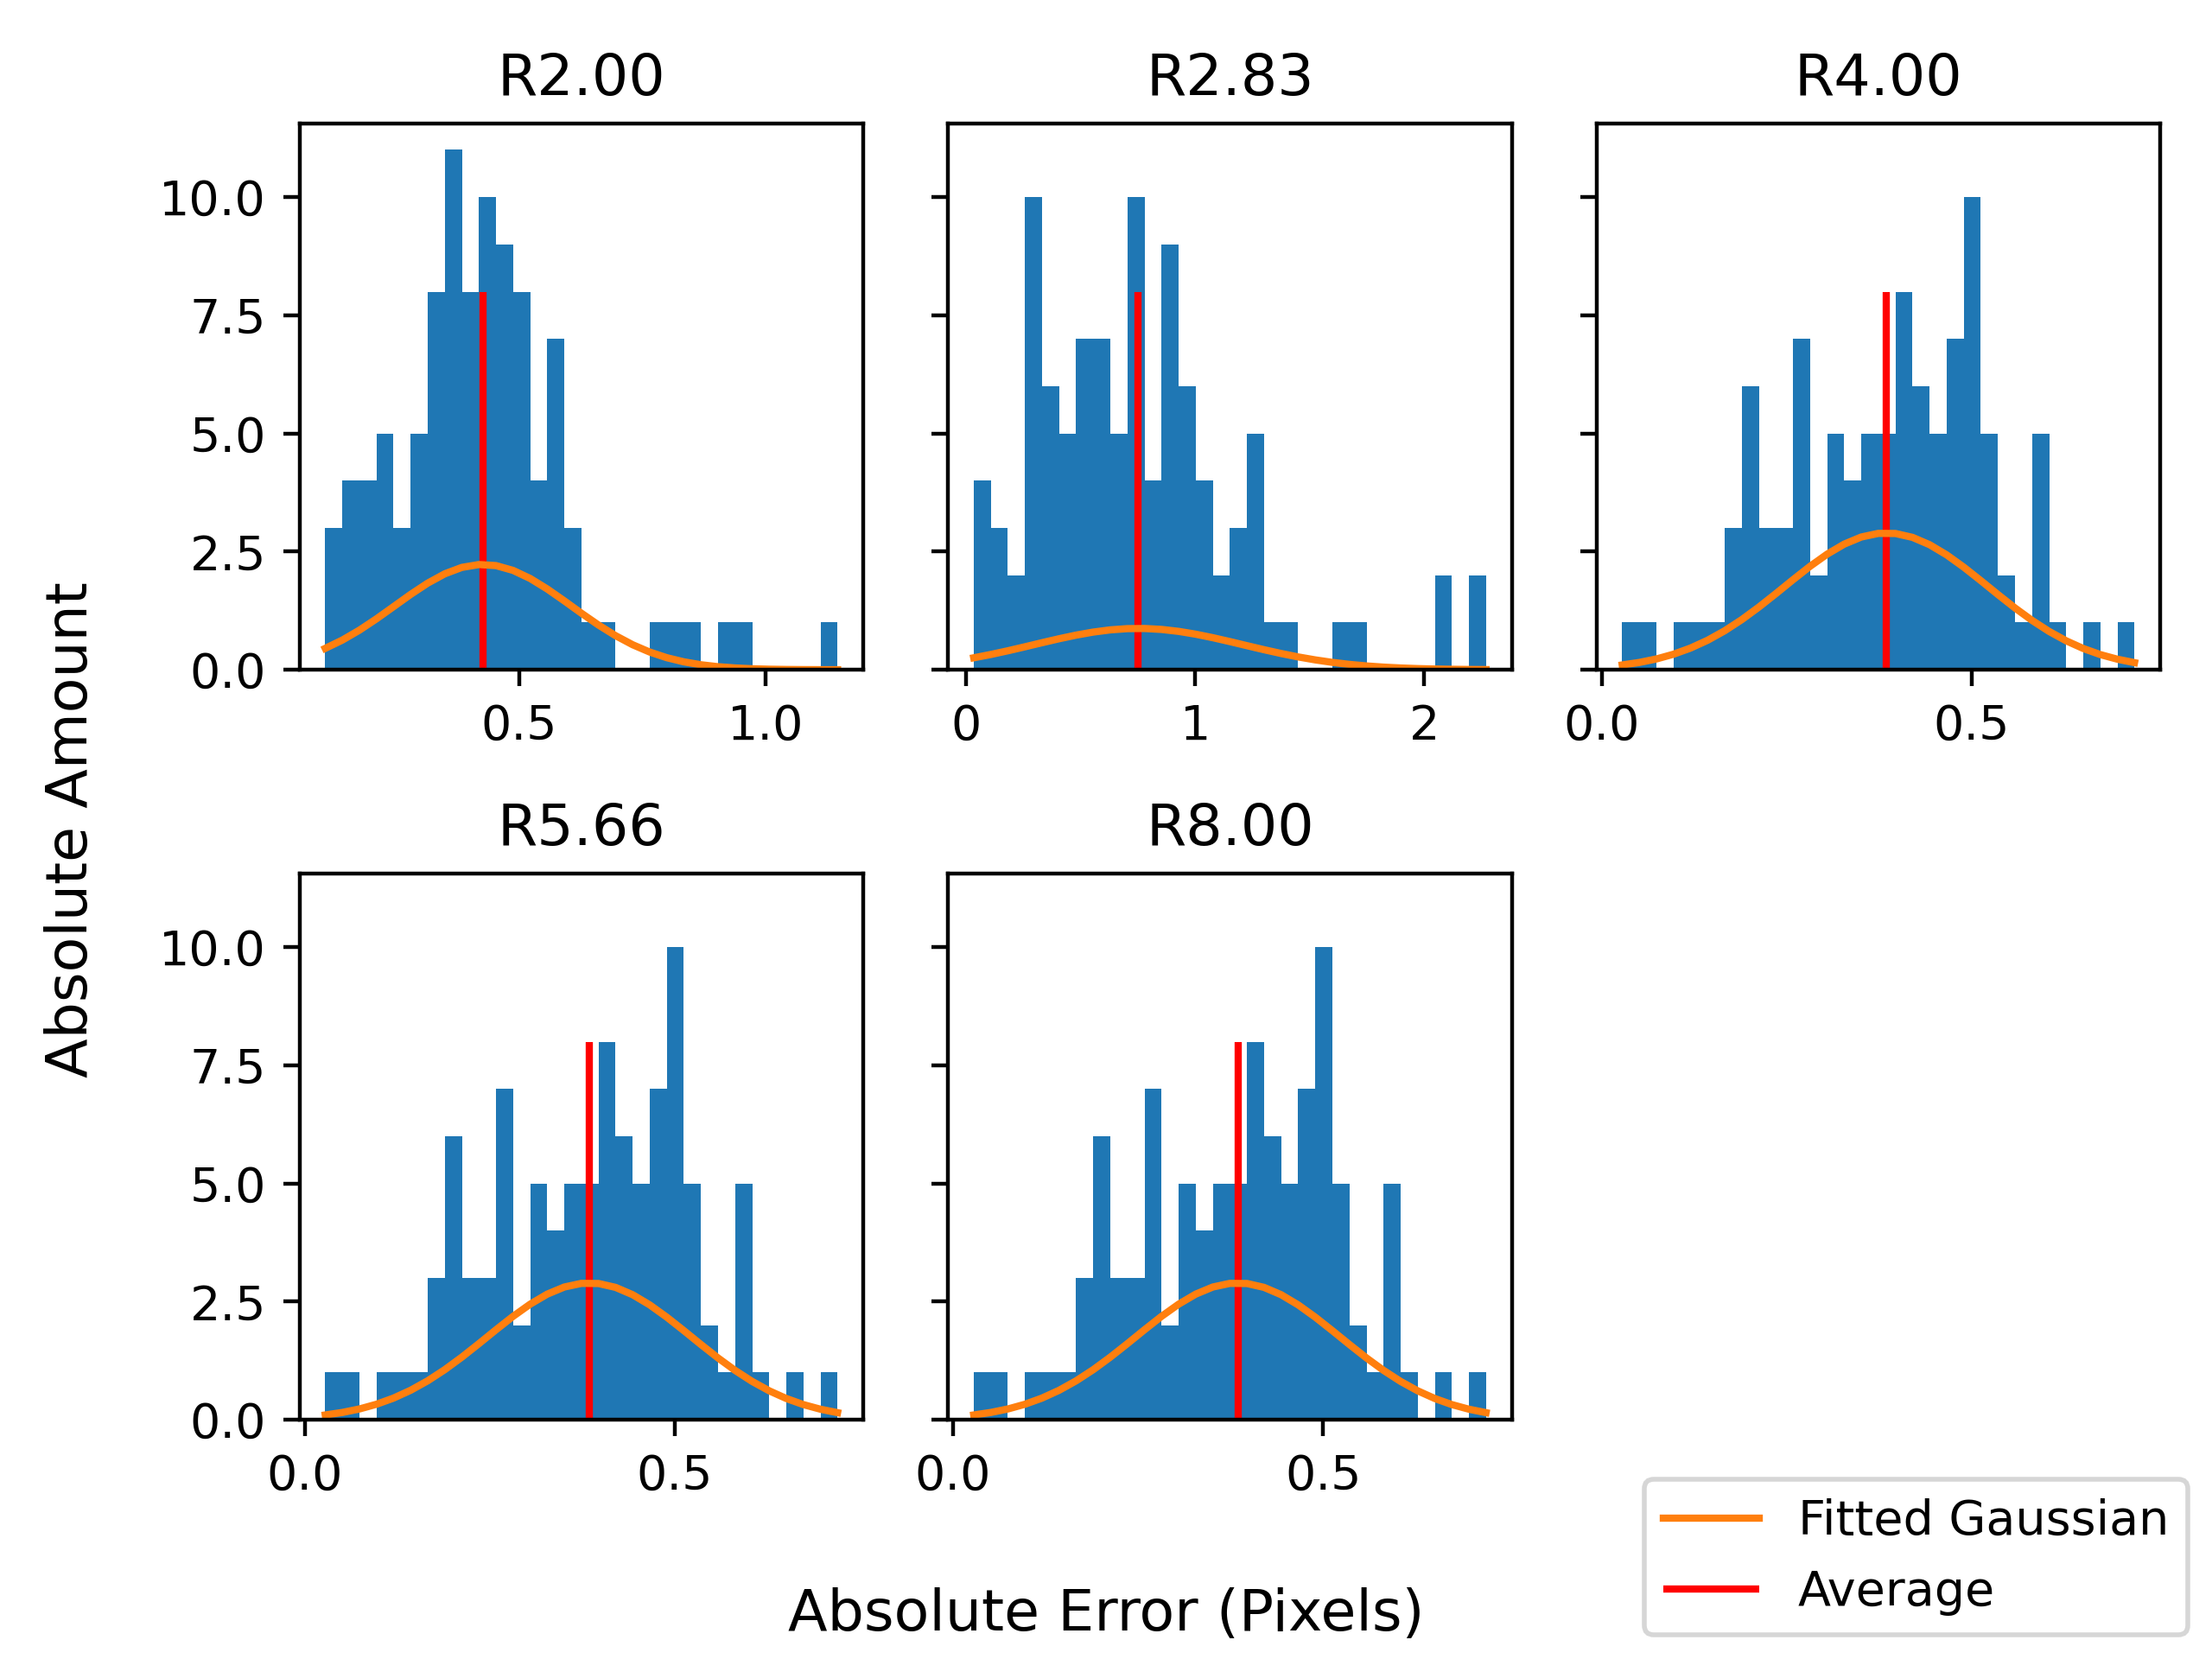
\includegraphics[width=0.7\textwidth]{project_pics/distro_noise.png}
    \end{center}
    \caption{Histograms of the absolute error from each radii, but with noise}
    \label{fig:distro_noise}
  \end{figure}


\section{Discussion} % (fold)
\label{sec:Discussion}


  In a paper by delabie et al. \cite{delabie2014accurate} known algorithms for spot finding were compiled 
  and tested for accuracy and efficiency, this includes variations of the centroid and Gaussian fit methods.
  The method used for centroiding that was used to test against the triangle method in this paper was attained 
  from delabie et al. \cite{delabie2014accurate} and was referred to as the centre of gravity method. In which when 
  it was tested it was found to take in the range of $0.055\rightarrow 0.253\cdot 10^{-6}$ seconds to calculate 
  the position of one star. This is in contrast with the time taken to calculate a single spot in this paper which 
  took $\approx 2\cdot 10^{-7}$ seconds, that's a $\approx 3.6\rightarrow 1$ times increase to a in elapsed 
  time. Comparing figure \ref{fig:box_var_r2} with figure 4 in the delabie et al. \cite{delabie2014accurate},
  star tracker data was used from the Plato mission which had had very little noise and gave very accurate estimates. 
  In comparison with figure \ref{fig:box_var_r2}, delabie et al. results had the same overall trend of gaining in accuracy 
  as box size increased, however the results that figure \ref{fig:box_var_r2} generated were larger in error. At it's 
  minimum error the centroiding algorithm employed here gave a result of $\approx 0.26$, while the minimum error 
  in the delabie et al. paper gave a result of $\approx 0.012$. 
  Now comparing figure \ref{fig:noise_box_r2} with figures 2 \& 3 in delabie et al. \cite{delabie2014accurate}, again 
  it can be seen that the general trend of the plots follows what was recreated here. In figure \ref{fig:noise_box_r2} 
  the minimum error achieved is $\approx 0.32$ with a box size of 7, in delabie et al. the minimum errors in figure 
  2 \& 3 are both $\approx 0.1$ whilst using a box size of 7. A reason for the discrepancy in both results may be due 
  to the data used, as for the centroiding methods, accuracy seems to be dependant the spot size in relation to the 
  box size. The elapsed time difference between the centroiding method and the triangle method were to be expected 
  from the outset, as the centroiding method has been used for star tracking from $1975 \rightarrow 1978$ and only 
  relies on two multiplications, two divisions and four summations to provide an answer. Centroiding is also 
  considered to be the fastest spot finding method.\cite{delabie2014accurate}

  A reason for the centroiding method and triangle method used in this paper being slower that others may 
  be due to the fact that the code for this paper was written in python, where as the centroiding method used in 
  delabie et al. was written in C$++$. Elapsed time test results taken from a website that poses the question 
  Which programming language is the fastest?\cite{bagley}, range from $\approx 2.5\rightarrow 95$ times 
  less time taken for C$++$ over python. This is however dependant on what is being ran, for example the largest 
  gap in elapsed time was from a symplectic-integrator that modeled planets and the smallest gap was from a program 
  that takes in strings of amino acid protein sequences and formats them. This means that what specific operations 
  are carried out on either language play a role in how fast the program runs, in part due to the fact that 
  python is an interpreted language whilst C$++$ is a compiled language.
  Another reason for this papers shortfall in computational time taken may be due to the use of python 
  packages used, this includes pandas, matplotlib, scipy, tifffile and others need to be called from 
  a different file. An improvement could be defining the functions that are used in the same file they are 
  being used in.

  A potential reason for the lack of accuracy in the method created could be attributed to the fact that 
  this method is a worse approximation of a spot than a Gaussian or an airy function. While these other 
  methods map more closely to a PSF, of which a diffraction limited point source of light follows, the triangle 
  method either over or under laps the shape of the spot (seen in figure \ref{fig:visual_test_2} \& \ref{fig:visual_test}) 
  possibly making a fitting function produce the errors observed.


  \subsection{Future work} % (fold)
  \label{sub:Discuss improvement}
  

  A possible fix for the current lack in accuracy with the triangle method could be modifying the 
  triangle function in a way that geometrically adds more area. This is to say that the shape of the function 
  should no longer just be a triangle but should also cover more area in a way that better fits an PSF. 
  This may fix the current accuracy issues as the under and overlap of area that a PSF and a triangle 
  have, may happen in such a way that disrupts the fitting function. The benefit that this would still 
  retain over a method like the Gaussian fitting one would be the area calculation, whilst being more complex, 
  would still be less computationally intensive than an integration. 

  Another idea that could potentially be worthwhile to investigate for spot finding could be using the pre-existing 
  method that works, for example Gaussian fitting, but trying to simplify it or approximate it. This could mean 
  producing a look up table of pre-calculated Gaussian functions that could be fitted to a spot. This would in theory 
  produce, provided a large enough look up table, a guess for the center of a spot with a similar accuracy to a 
  normally fitted and integrated function, whilst also having a elapsed time advantage. 



  
% subsection subsection name (end)


\section{Conclusion} % (fold)
\label{sec:Conclusion}

  To conclude a spot finding method was created and others were replicated in order to compare 
  accuracy and time taken. In section \ref{sec:intro} important concepts about sub-pixel localisation 
  were discussed to give an overarching view what it is and why this paper was trying to improve it 
  in some manner. In section \ref{sec:Methods} the procedures that were carried out like centroiding 
  and the Gaussian fitting method were explained step by step to understand the apparent costs and benefits 
  of well understood and common place algorithms. Furthermore a new method was created and discussed in order 
  to align with the motivation behind the study of trying to produce a method that is still fast in terms 
  of time taken to give an answer but also more accurate than an algorithm like centroiding. In section \ref{sec:Results}
  the centroiding and triangle algorithms were tested with spot data provided, for the simulated perfect data this resulted 
  in the centroiding algorithm predictably being faster (16500 times) and being more accurate ($\approx 19\rightarrow 1.25$ times) 
  except from the case of the 3x3 box size where the triangle method has better accuracy ($\approx 1.33\rightarrow 2.6$ times).
  In the case of the simulated noisy data, again, the centroiding method takes the advantage with results more 
  accurate ($\approx 1.5\rightarrow 2$ times). Additionally in section \ref{sec:Discussion} we discussed potential 
  reasons on why the method created and other methods used perform worse than methods executed in cited papers. 
  Following this critique in section \ref{sub:Discuss improvement} improvements were discussed that will be investigated 
  further in future work to be conducted. Overall, even though the method created failed to produce better results 
  than initially hoped, it still shows promise and demands further study. During the process of this paper I have 
  greatly expanded my knowledge of microscopy, fluorescence, computing and in general how to develop methods to 
  try and solve problems. 

% section :Conclusion (end)



\newpage
\bibliographystyle{unsrt}
\bibliography{myreferences}%reads a .bib file called myreferences.bib for the actual references in BibTeX format. You can call your BibTeX file something else if you prefer.
\addcontentsline{toc}{section}{References}
%If there are problems with compiling the LaTeX file with BibTeX, make sure that file names don't have spaces in them as this might cause problems

\newpage
\appendix

\section{Appendix}
\label{sec:appendix}
%%% centroiding appendix part

  All code developed or used for this project is available on GitHub along with the spot data generated.
  \url{https://github.com/AntonGashi/4th_year_project}

  \begin{figure}[H]
    \begin{center}
      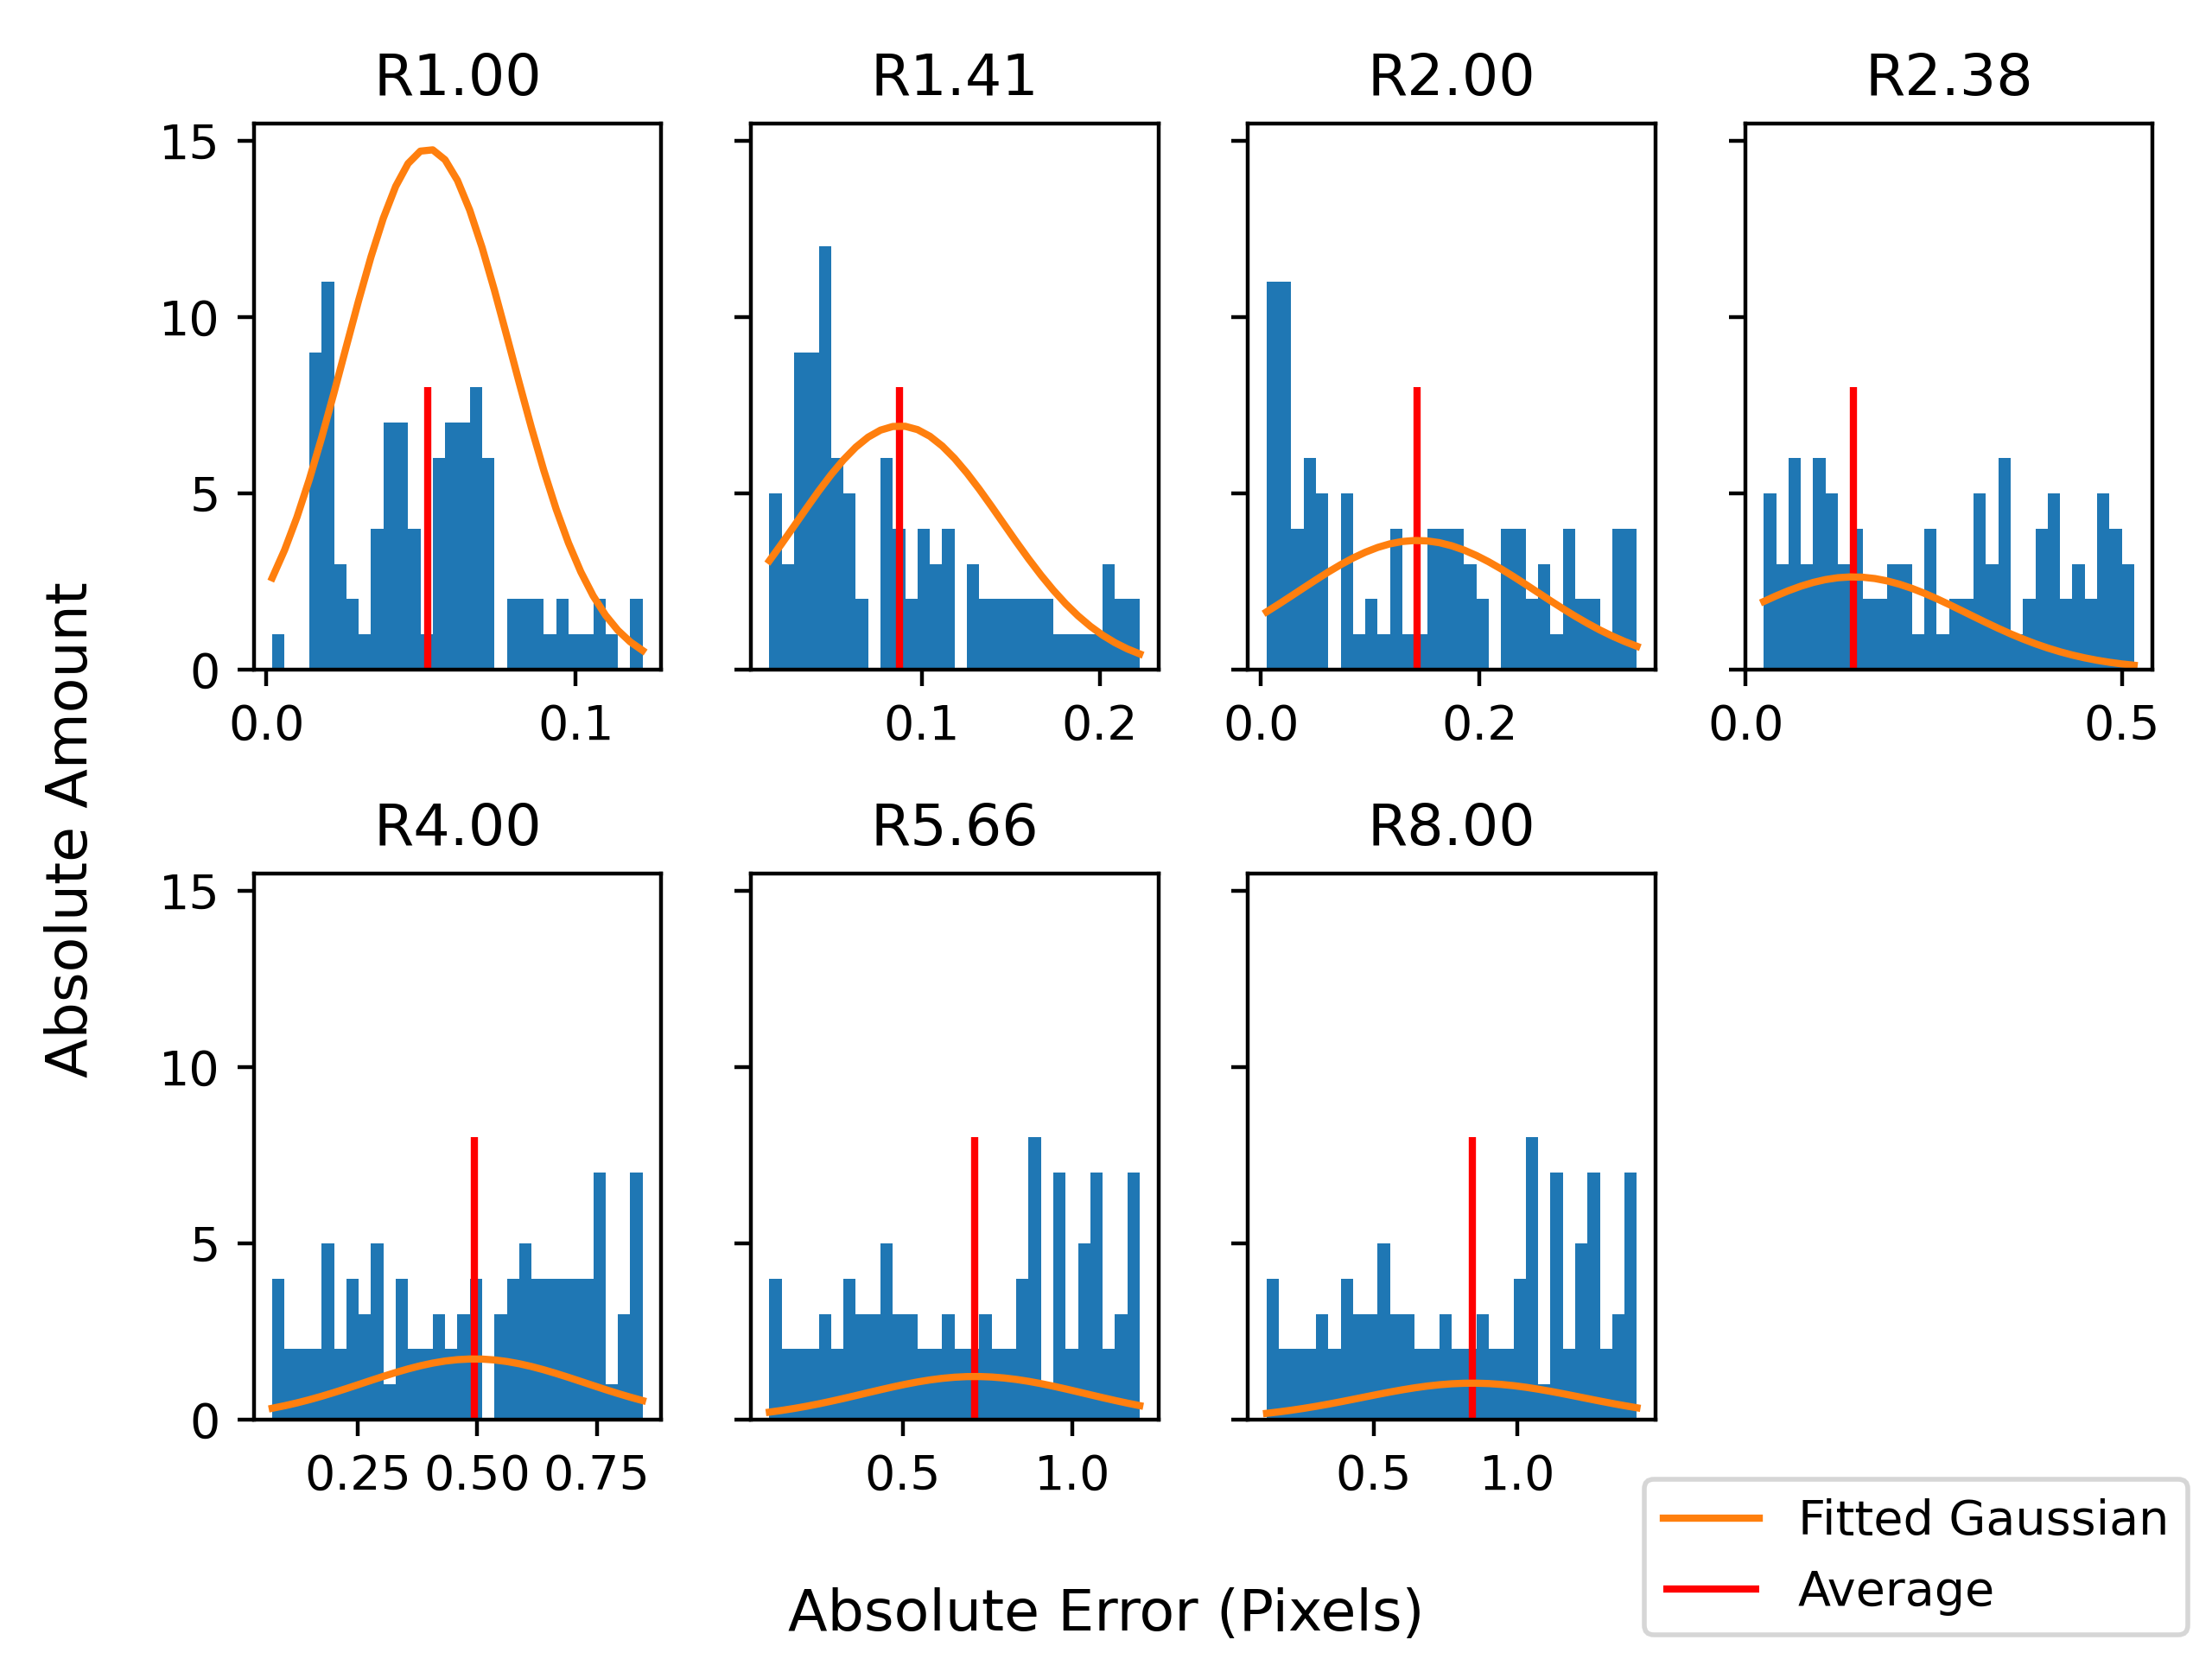
\includegraphics[width=0.6\textwidth]{project_pics/distro_centriod_5.png}
    \end{center}
    \caption{Histograms of the absolute error from each radii with a box size of 5x5 pixels.}
    \label{fig:box_5}
  \end{figure}

  \begin{figure}[H]
    \begin{center}
      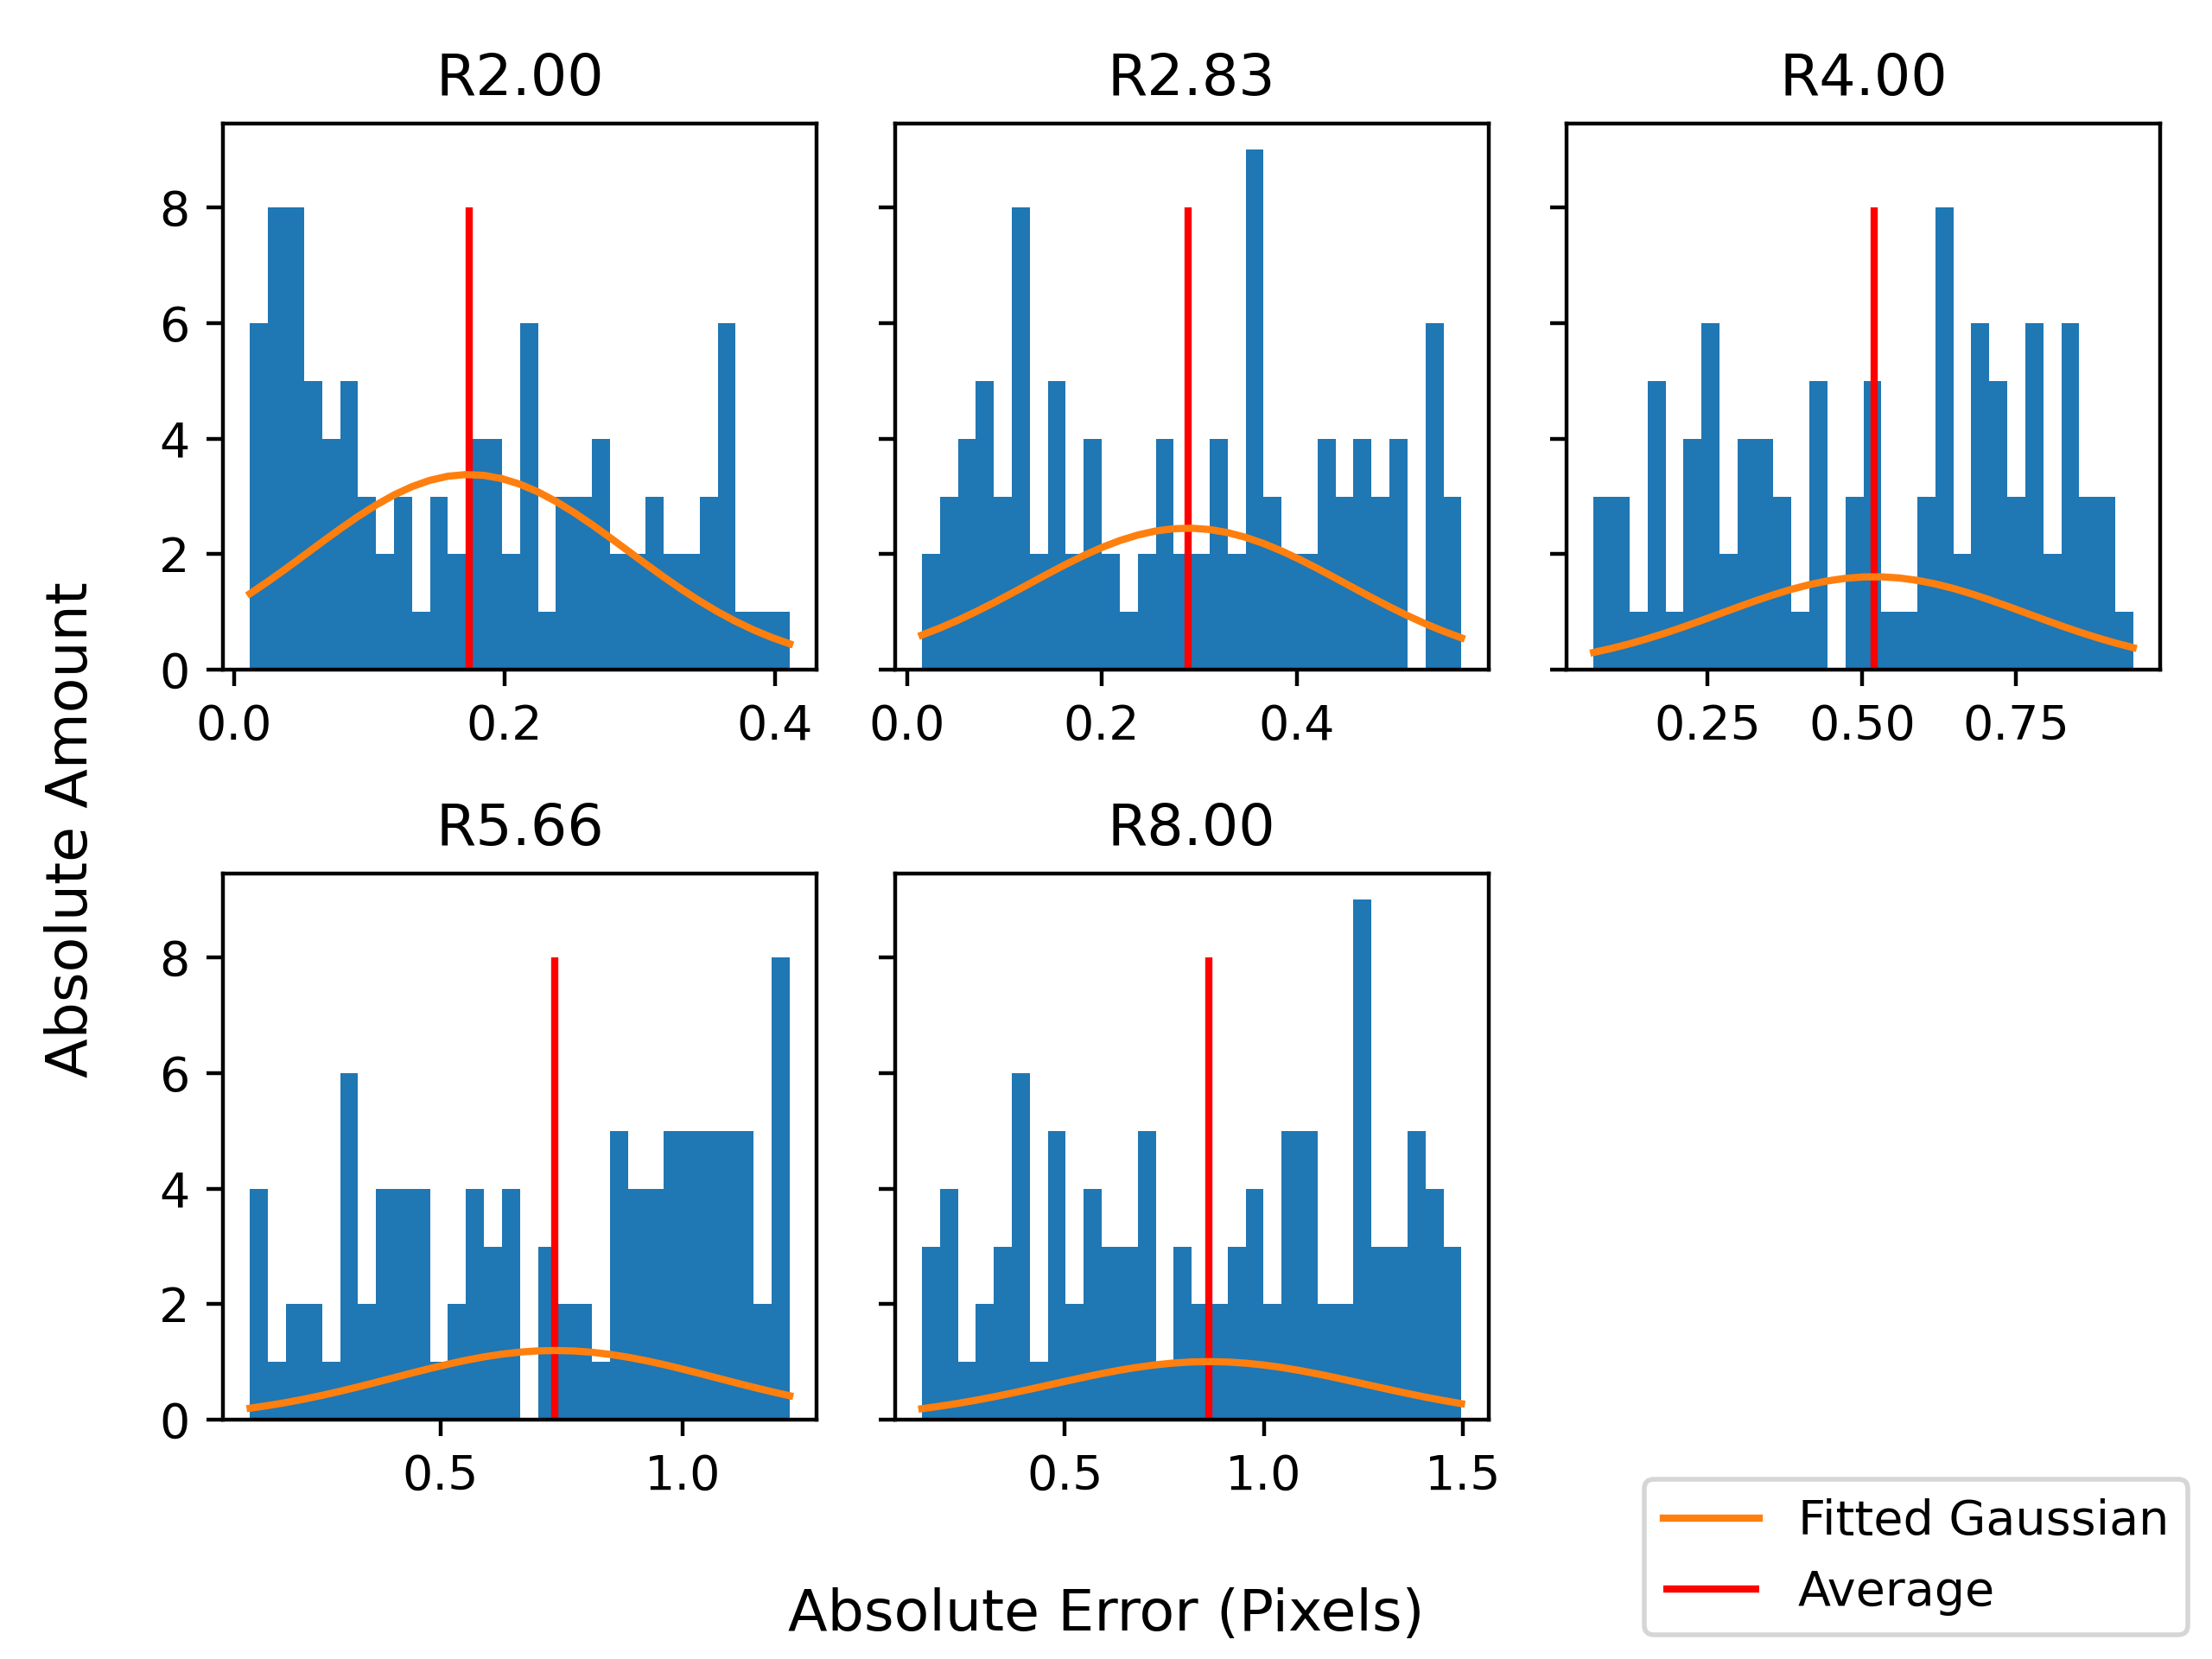
\includegraphics[width=0.6\textwidth]{project_pics/noise_cen_scatter_5.png}
    \end{center}
    \caption{Histograms of the absolute error from each radii with a box size of 5x5 pixels, with noise.}
    \label{fig:box_5_noise}
  \end{figure}

  \begin{figure}[H]
    \begin{center}
      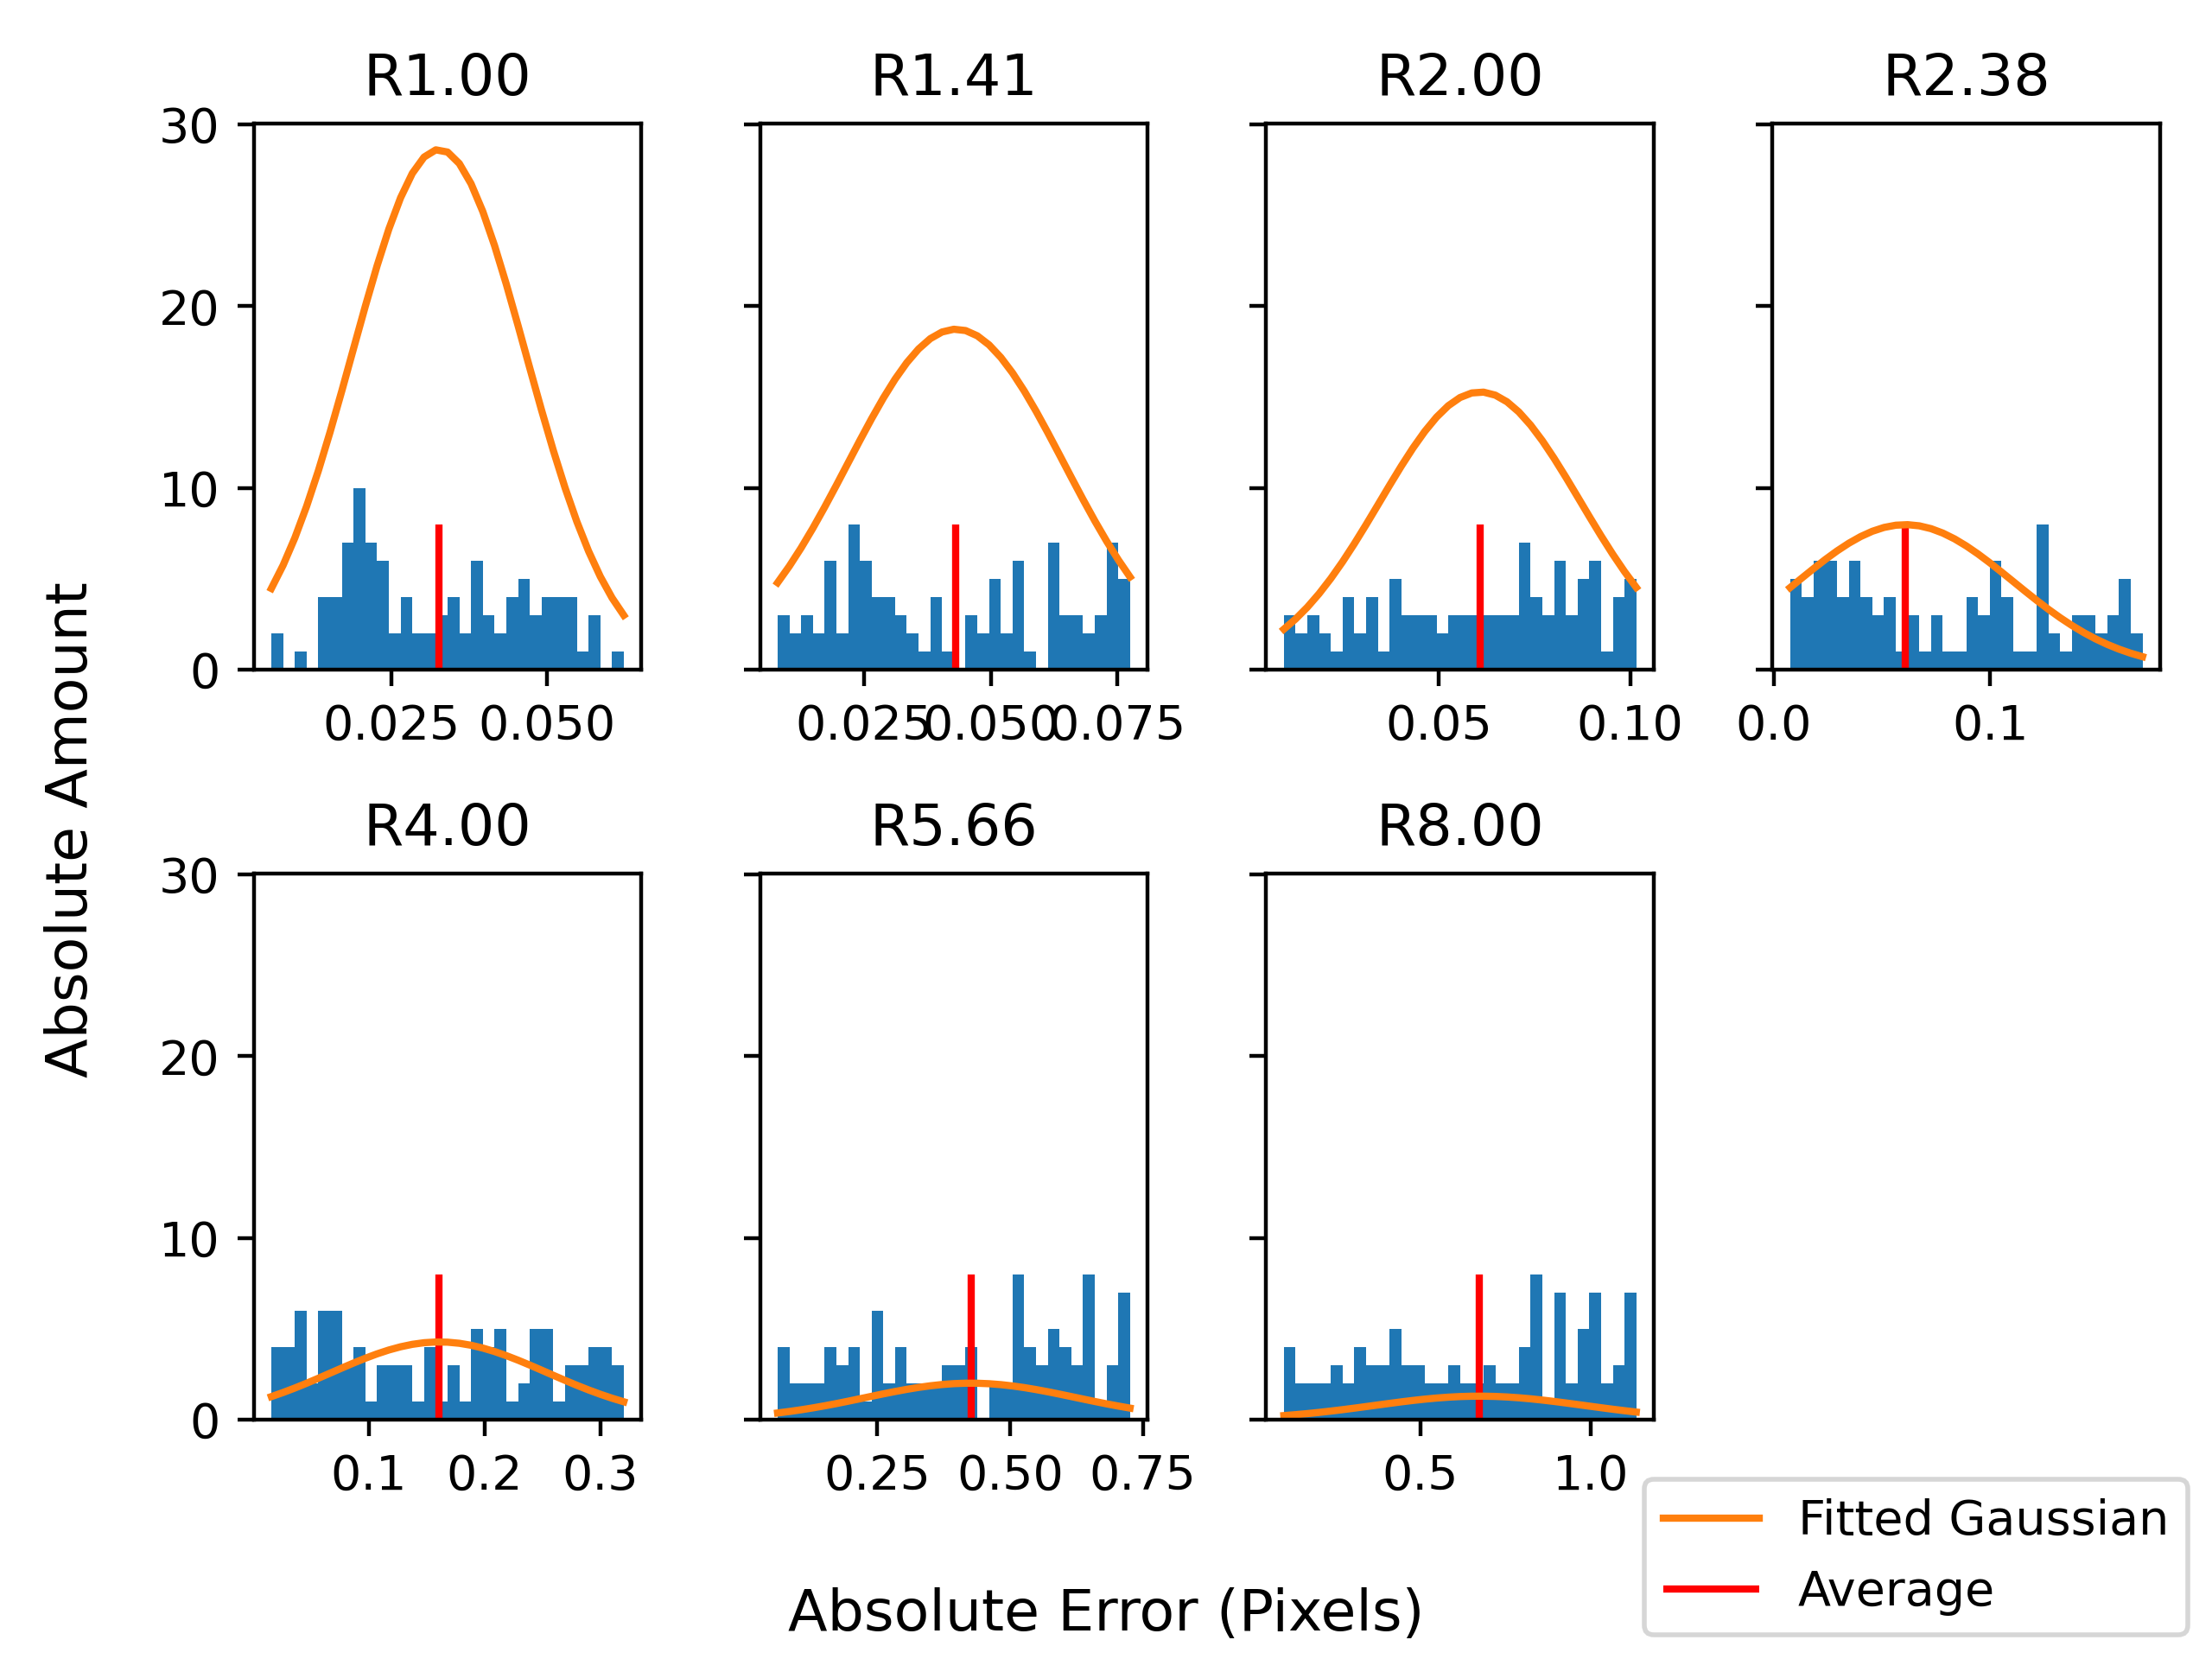
\includegraphics[width=0.6\textwidth]{project_pics/distro_centriod_7.png}
    \end{center}
    \caption{Histograms of the absolute error from each radii with a box size of 7x7 pixels.}
    \label{fig:box_7}
  \end{figure}

  \begin{figure}[H]
    \begin{center}
      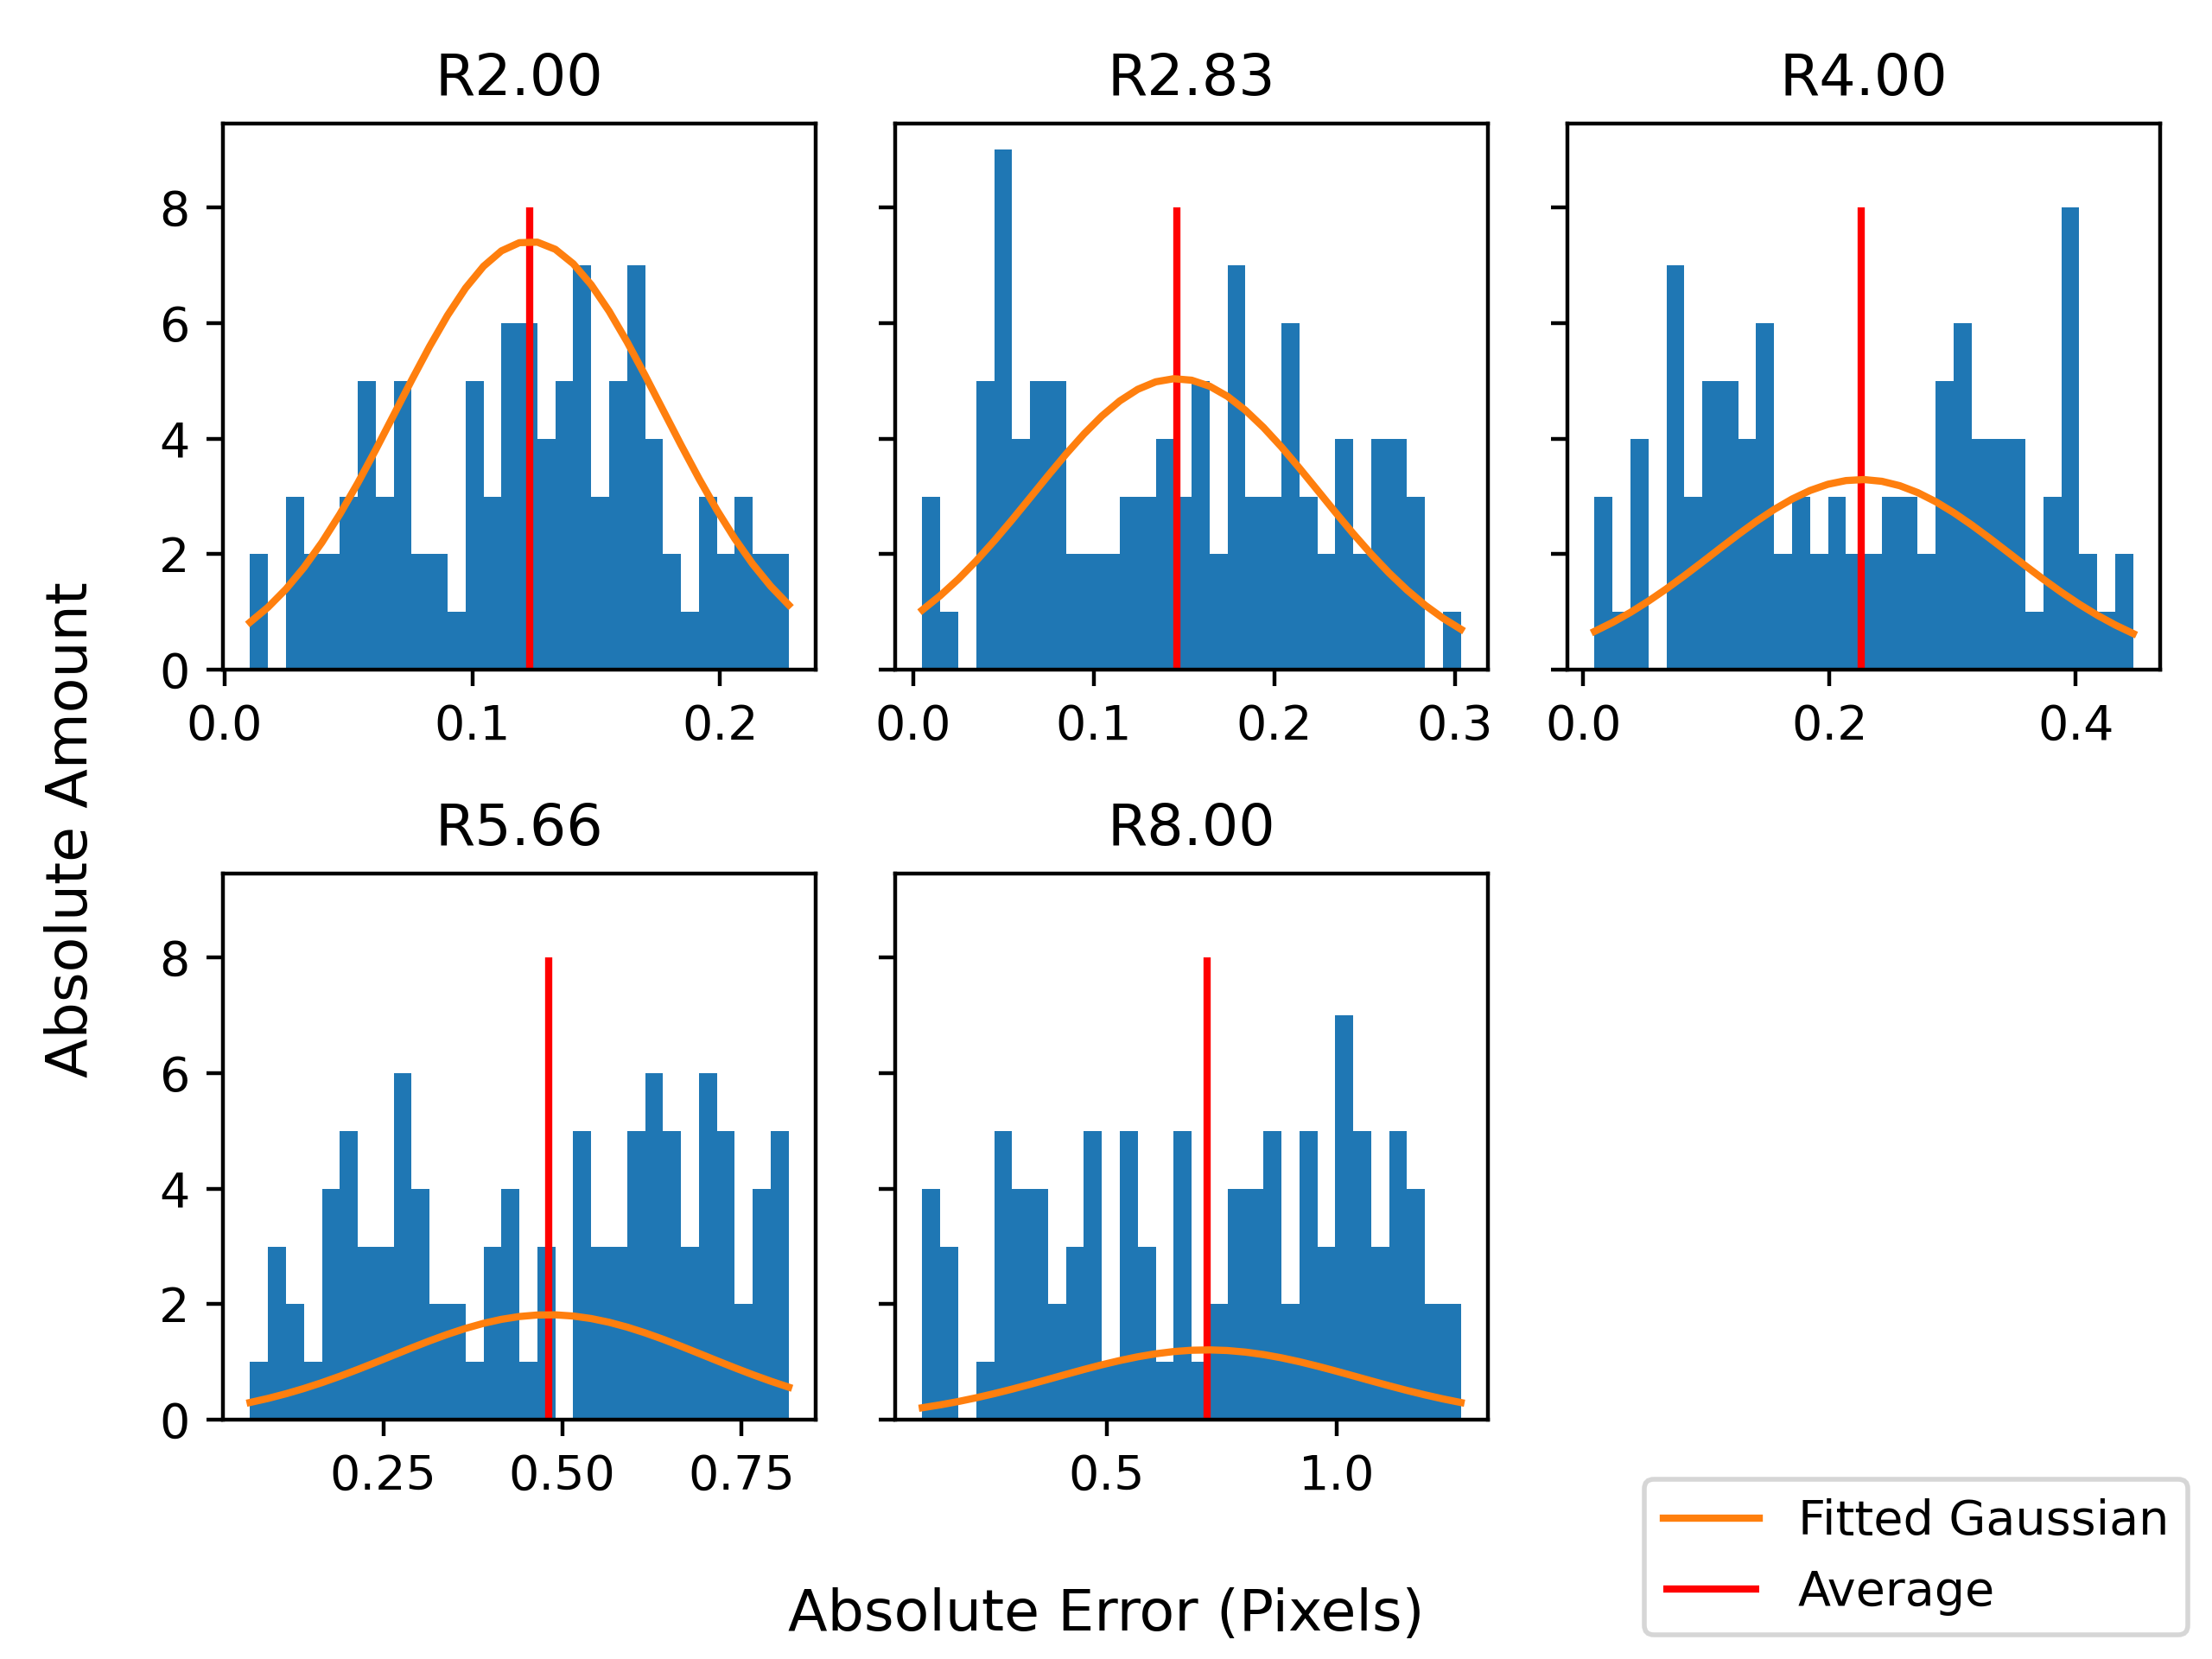
\includegraphics[width=0.6\textwidth]{project_pics/noise_cen_scatter_7.png}
    \end{center}
    \caption{Histograms of the absolute error from each radii with a box size of 7x7 pixels, with noise.}
    \label{fig:box_7_noise}
  \end{figure}
%%% centroiding appendix part end 

  \begin{figure}[H]
      \begin{center}
        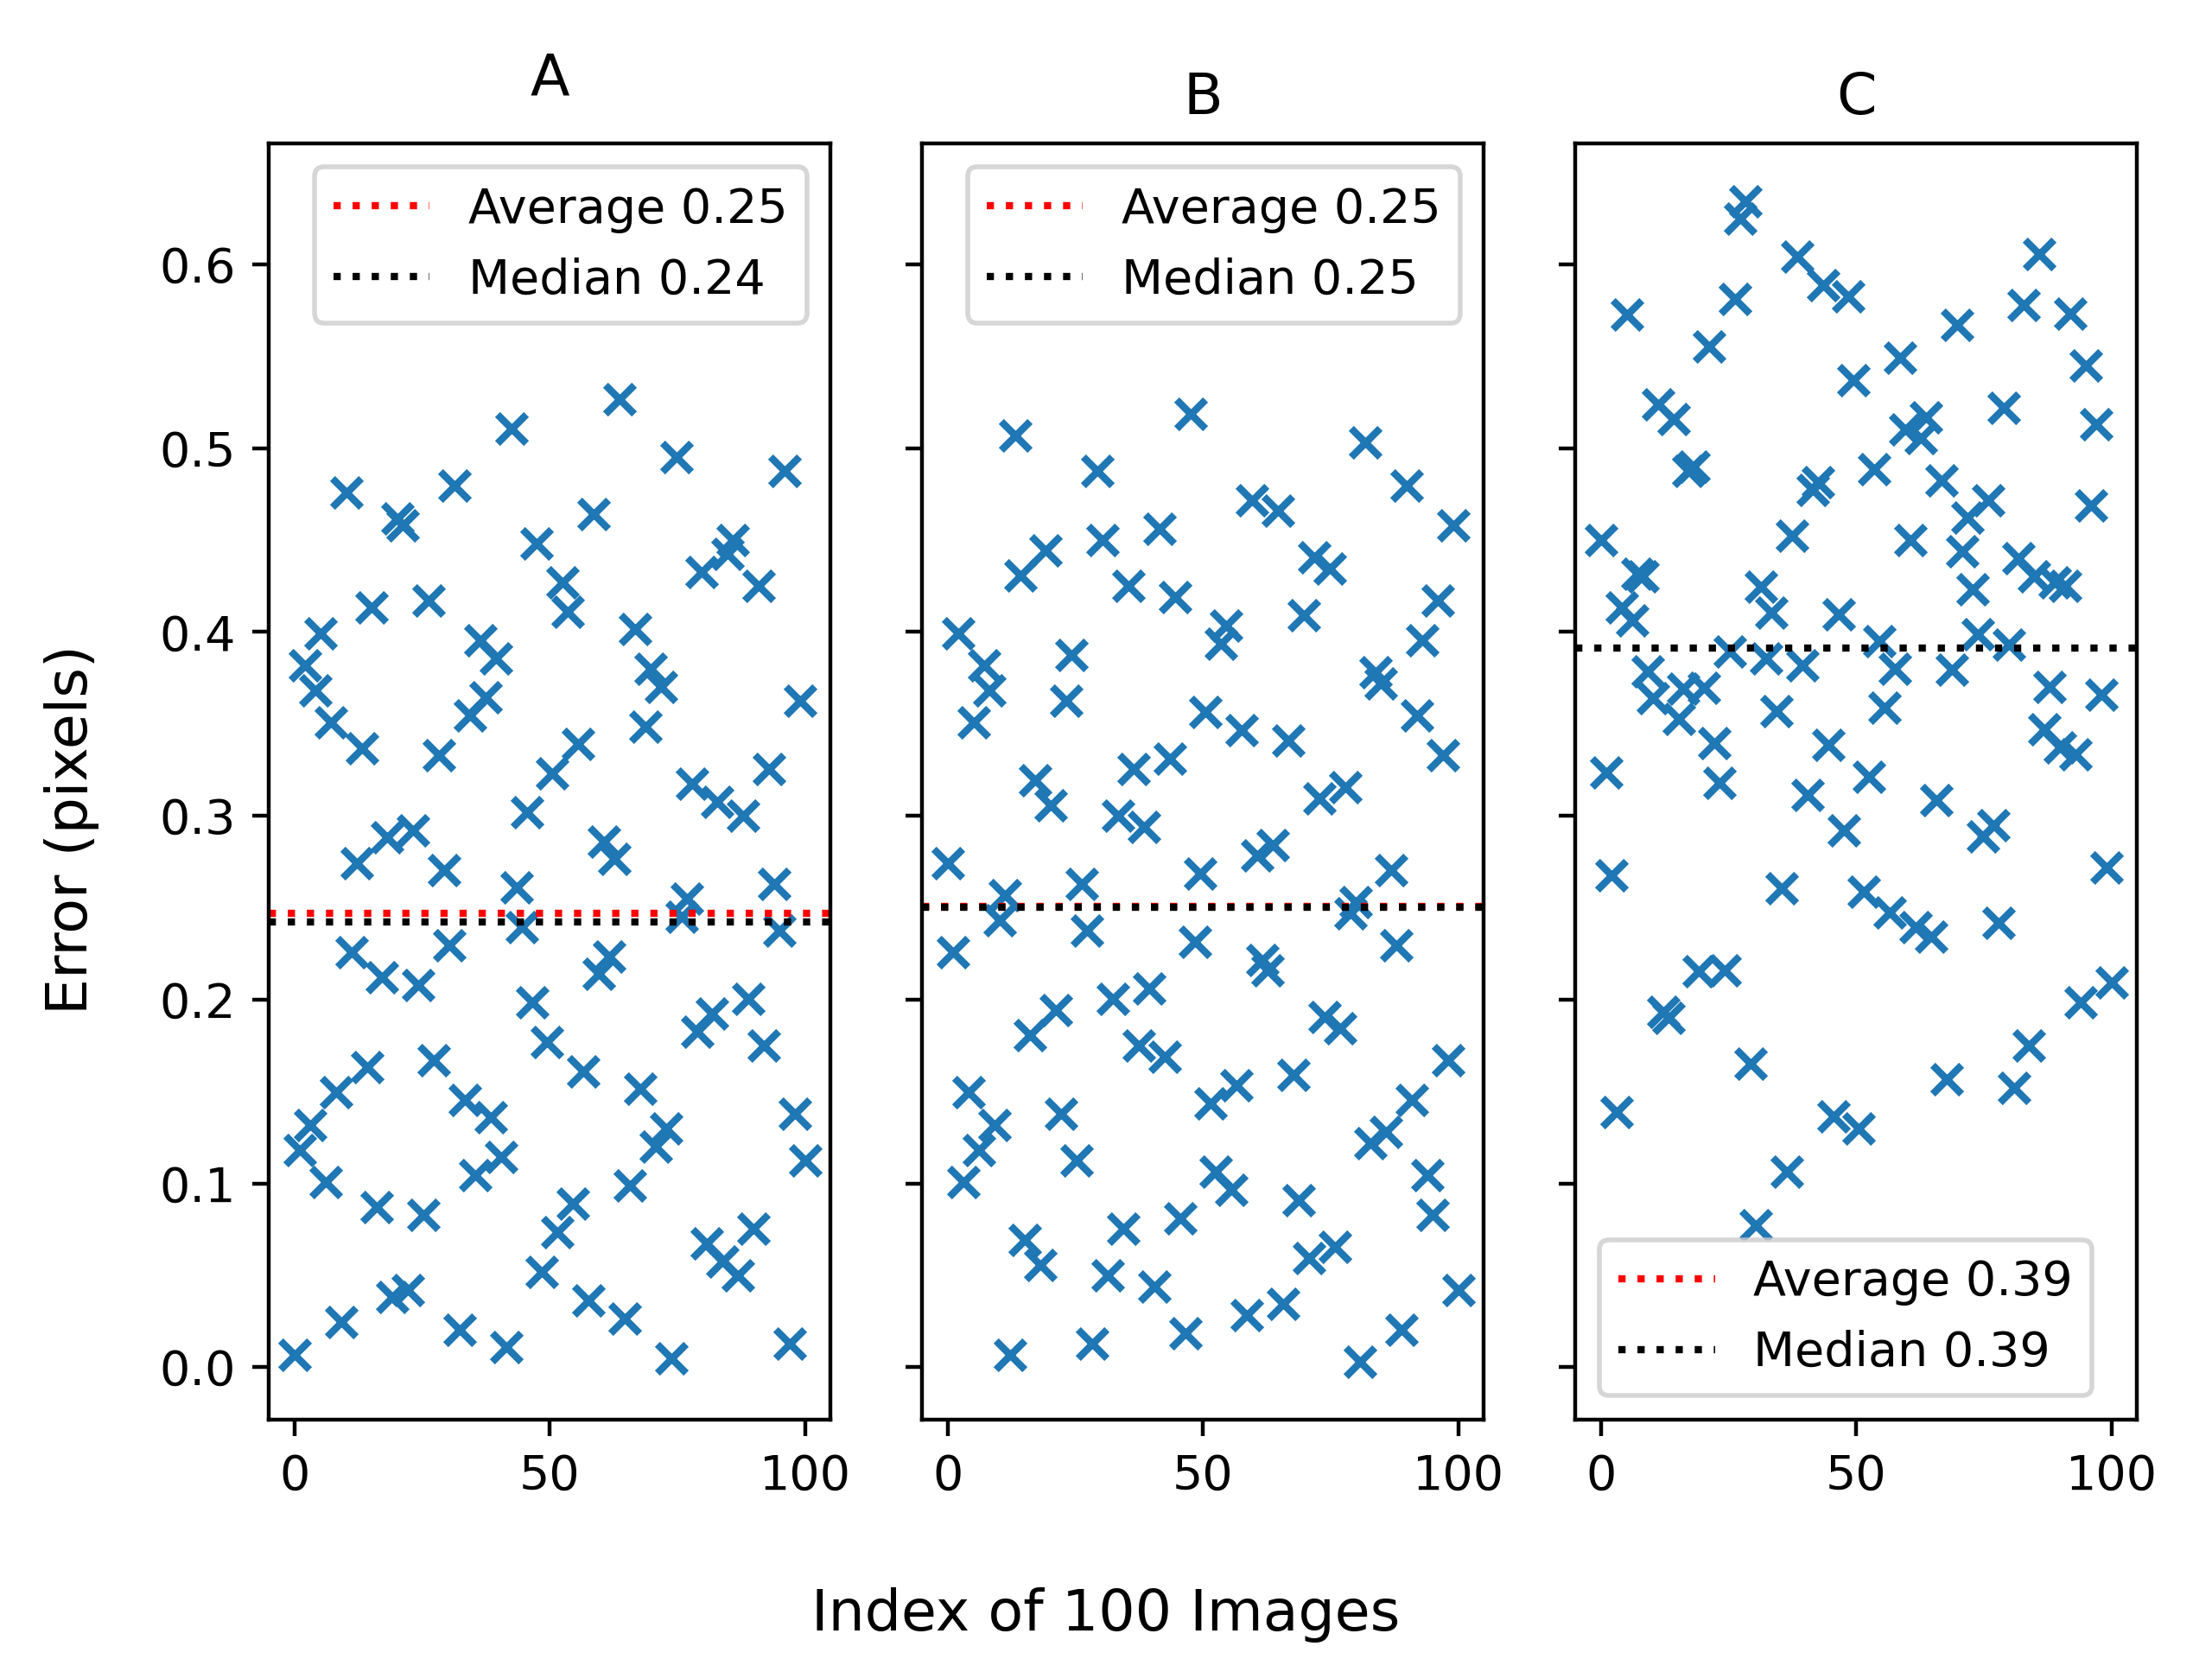
\includegraphics[width=0.7\textwidth]{project_pics/single_test.png}
      \end{center}
      \caption{Simulated spots with R1.00, A: Error in the X direction, B: Error in the Y direction, C: Absolute error from the ground-truth}
      \label{fig:single_test}
    \end{figure}

  \begin{figure}[H]
    \begin{center}
      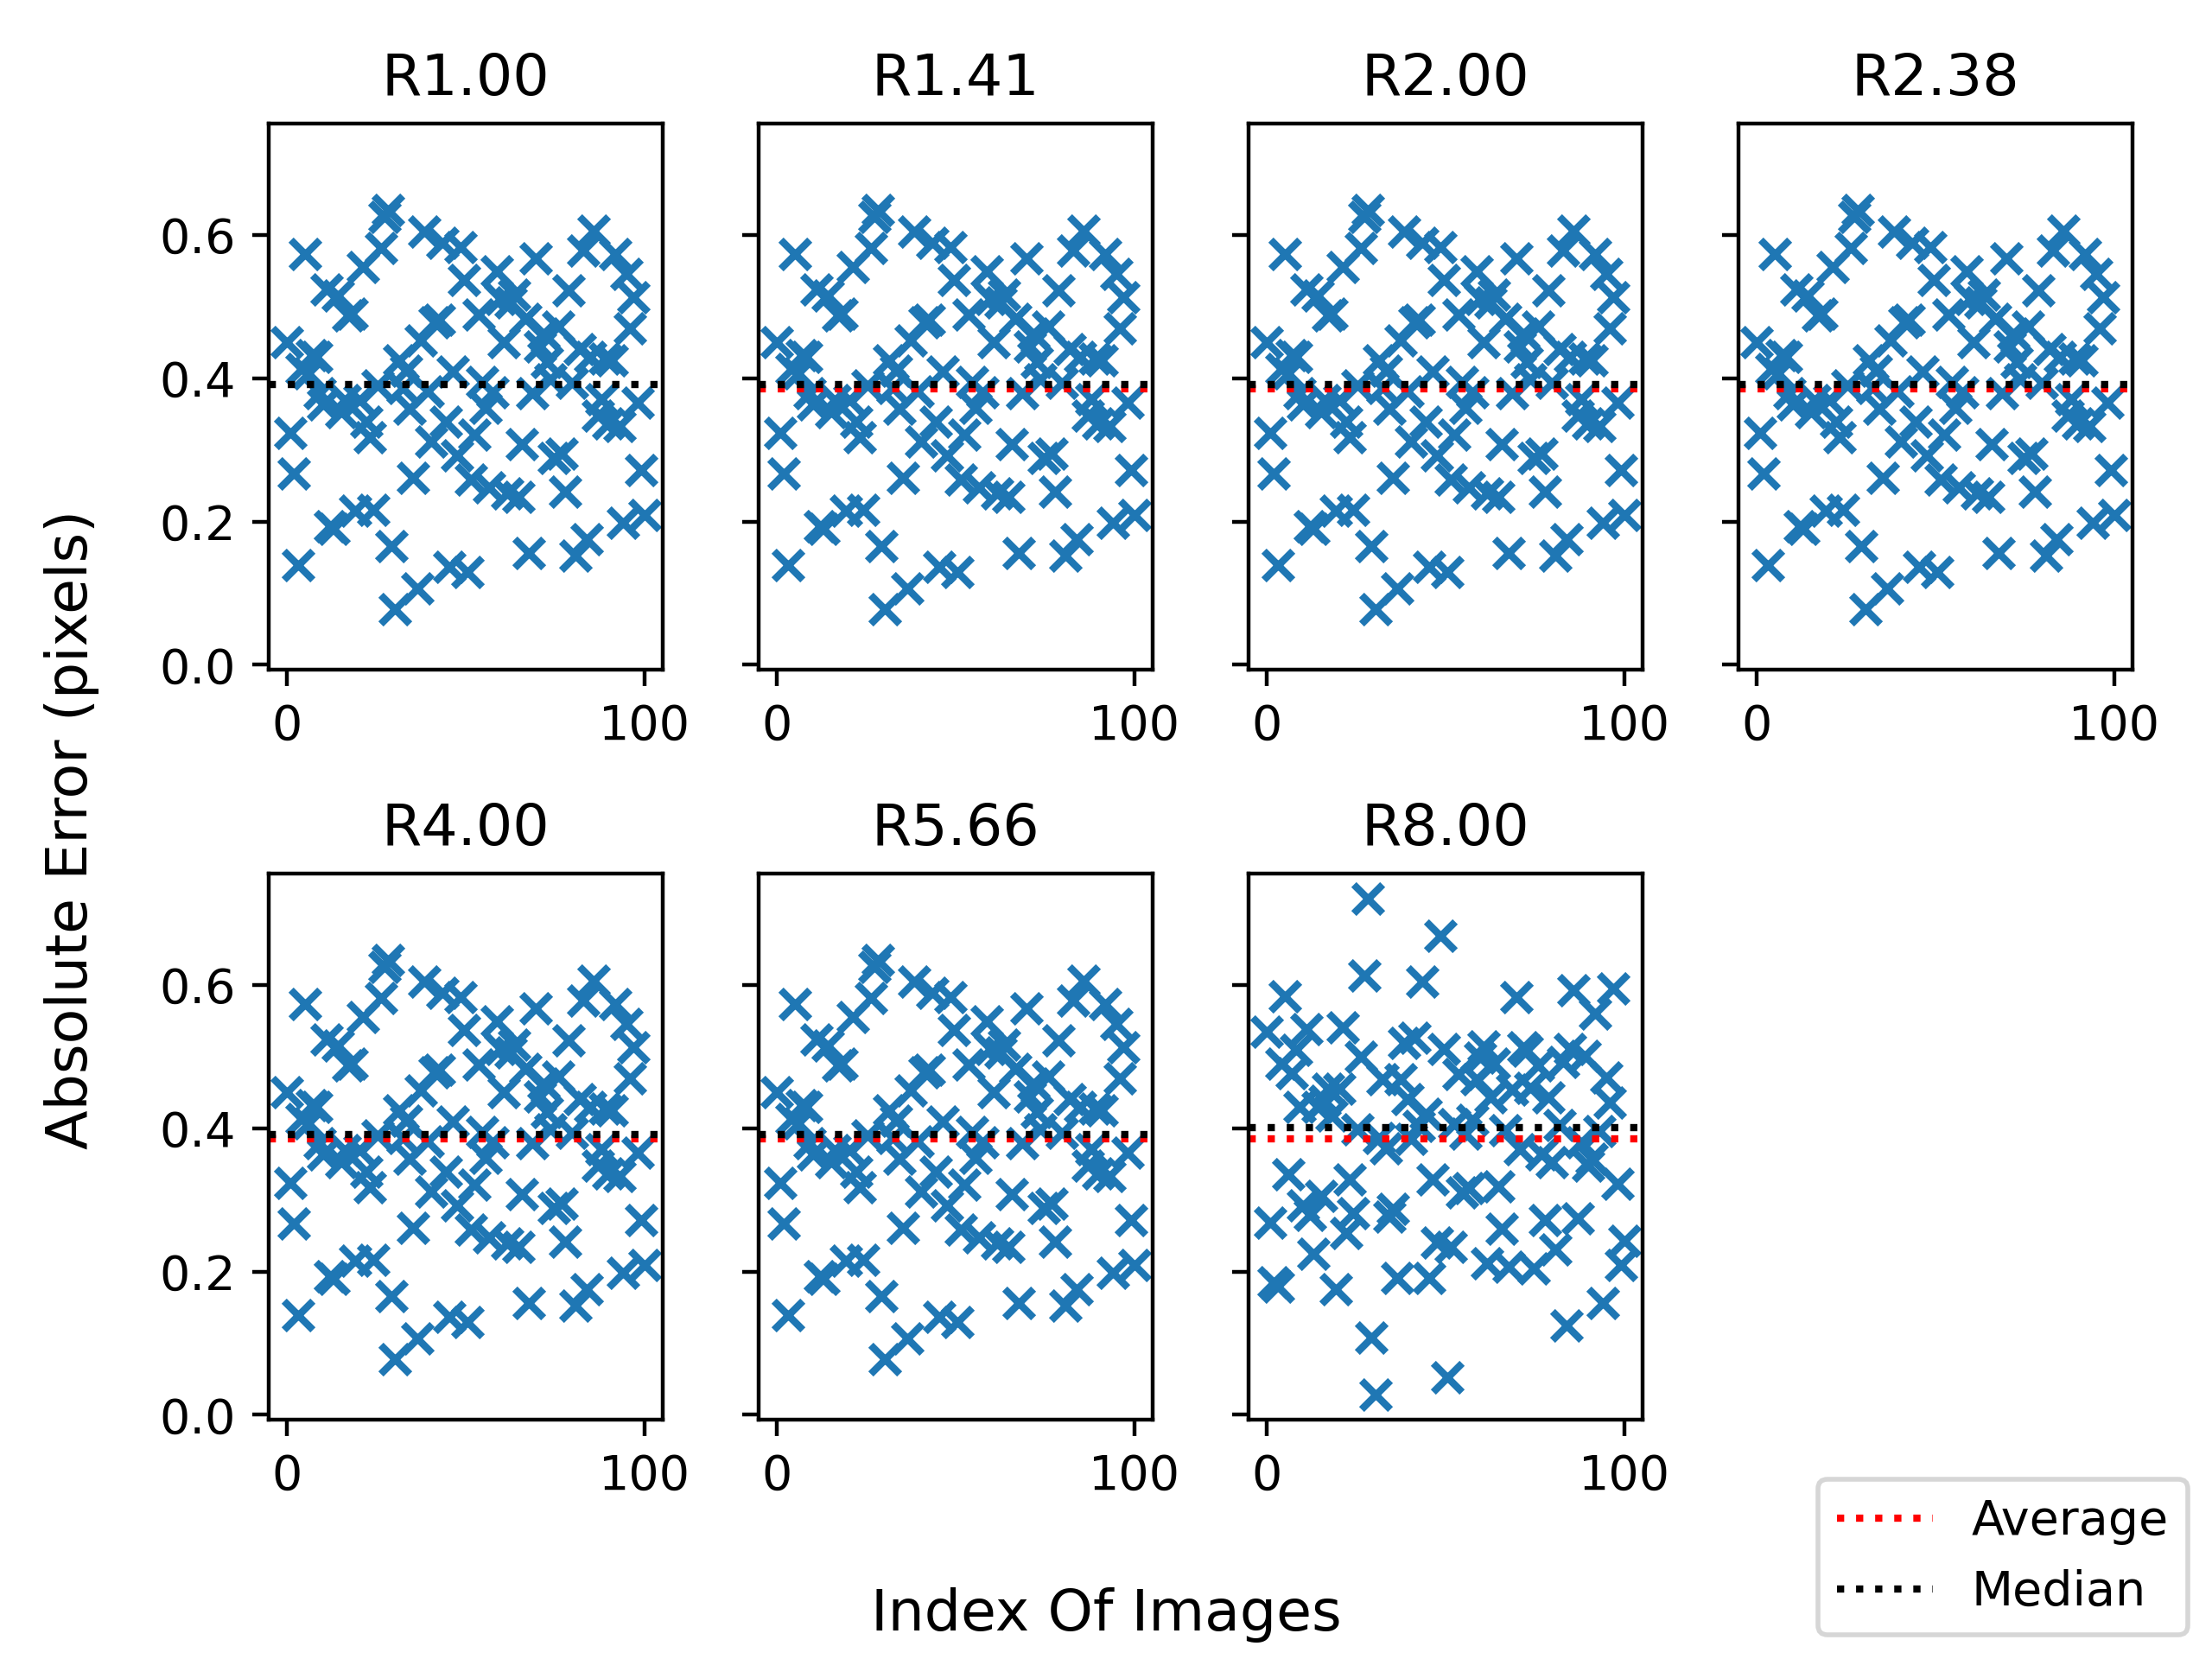
\includegraphics[width=0.7\textwidth]{project_pics/no_noise_all_r.png}
    \end{center}
    \caption{Spot localisation (like graph C in figure \ref{fig:single_test}) of different radii, R, on perfect data (executed in 2.4s)}
    \label{fig:no_noise_all_r}
  \end{figure}

 \begin{figure}[H]
   \begin{center}
     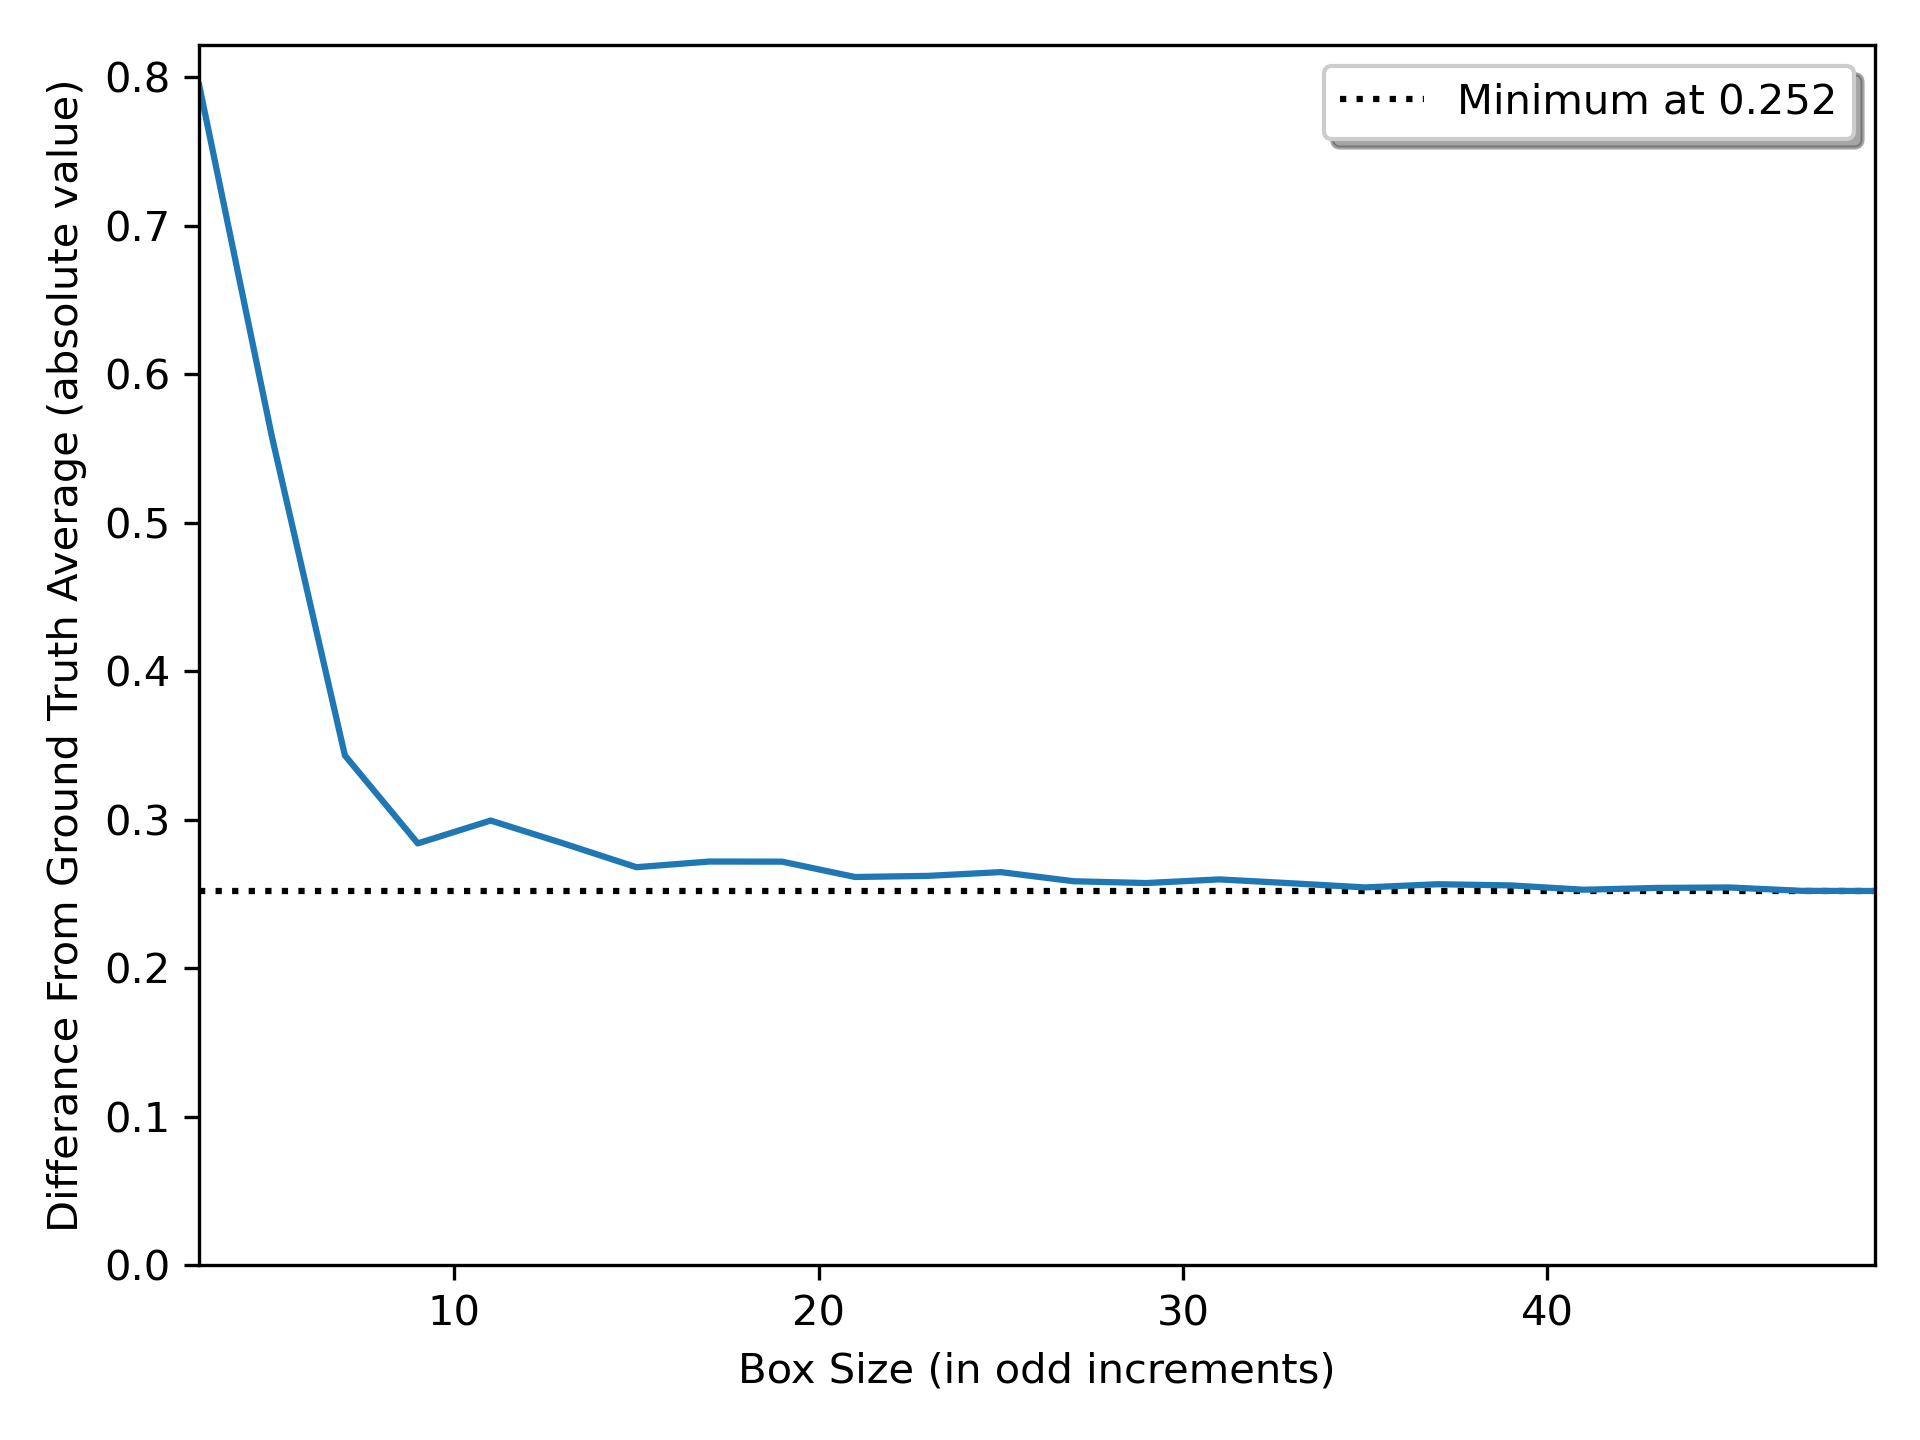
\includegraphics[width=0.7\textwidth]{project_pics/box_size_var_r4.png}
   \end{center}
   \caption{Showing the accuracy of centroiding Vs the box size chosen (from 3 to 49), for a radii or R4.00 and without noise}
   \label{fig:box_size_var_r4}
 \end{figure}

 \begin{figure}[H]
   \begin{center}
     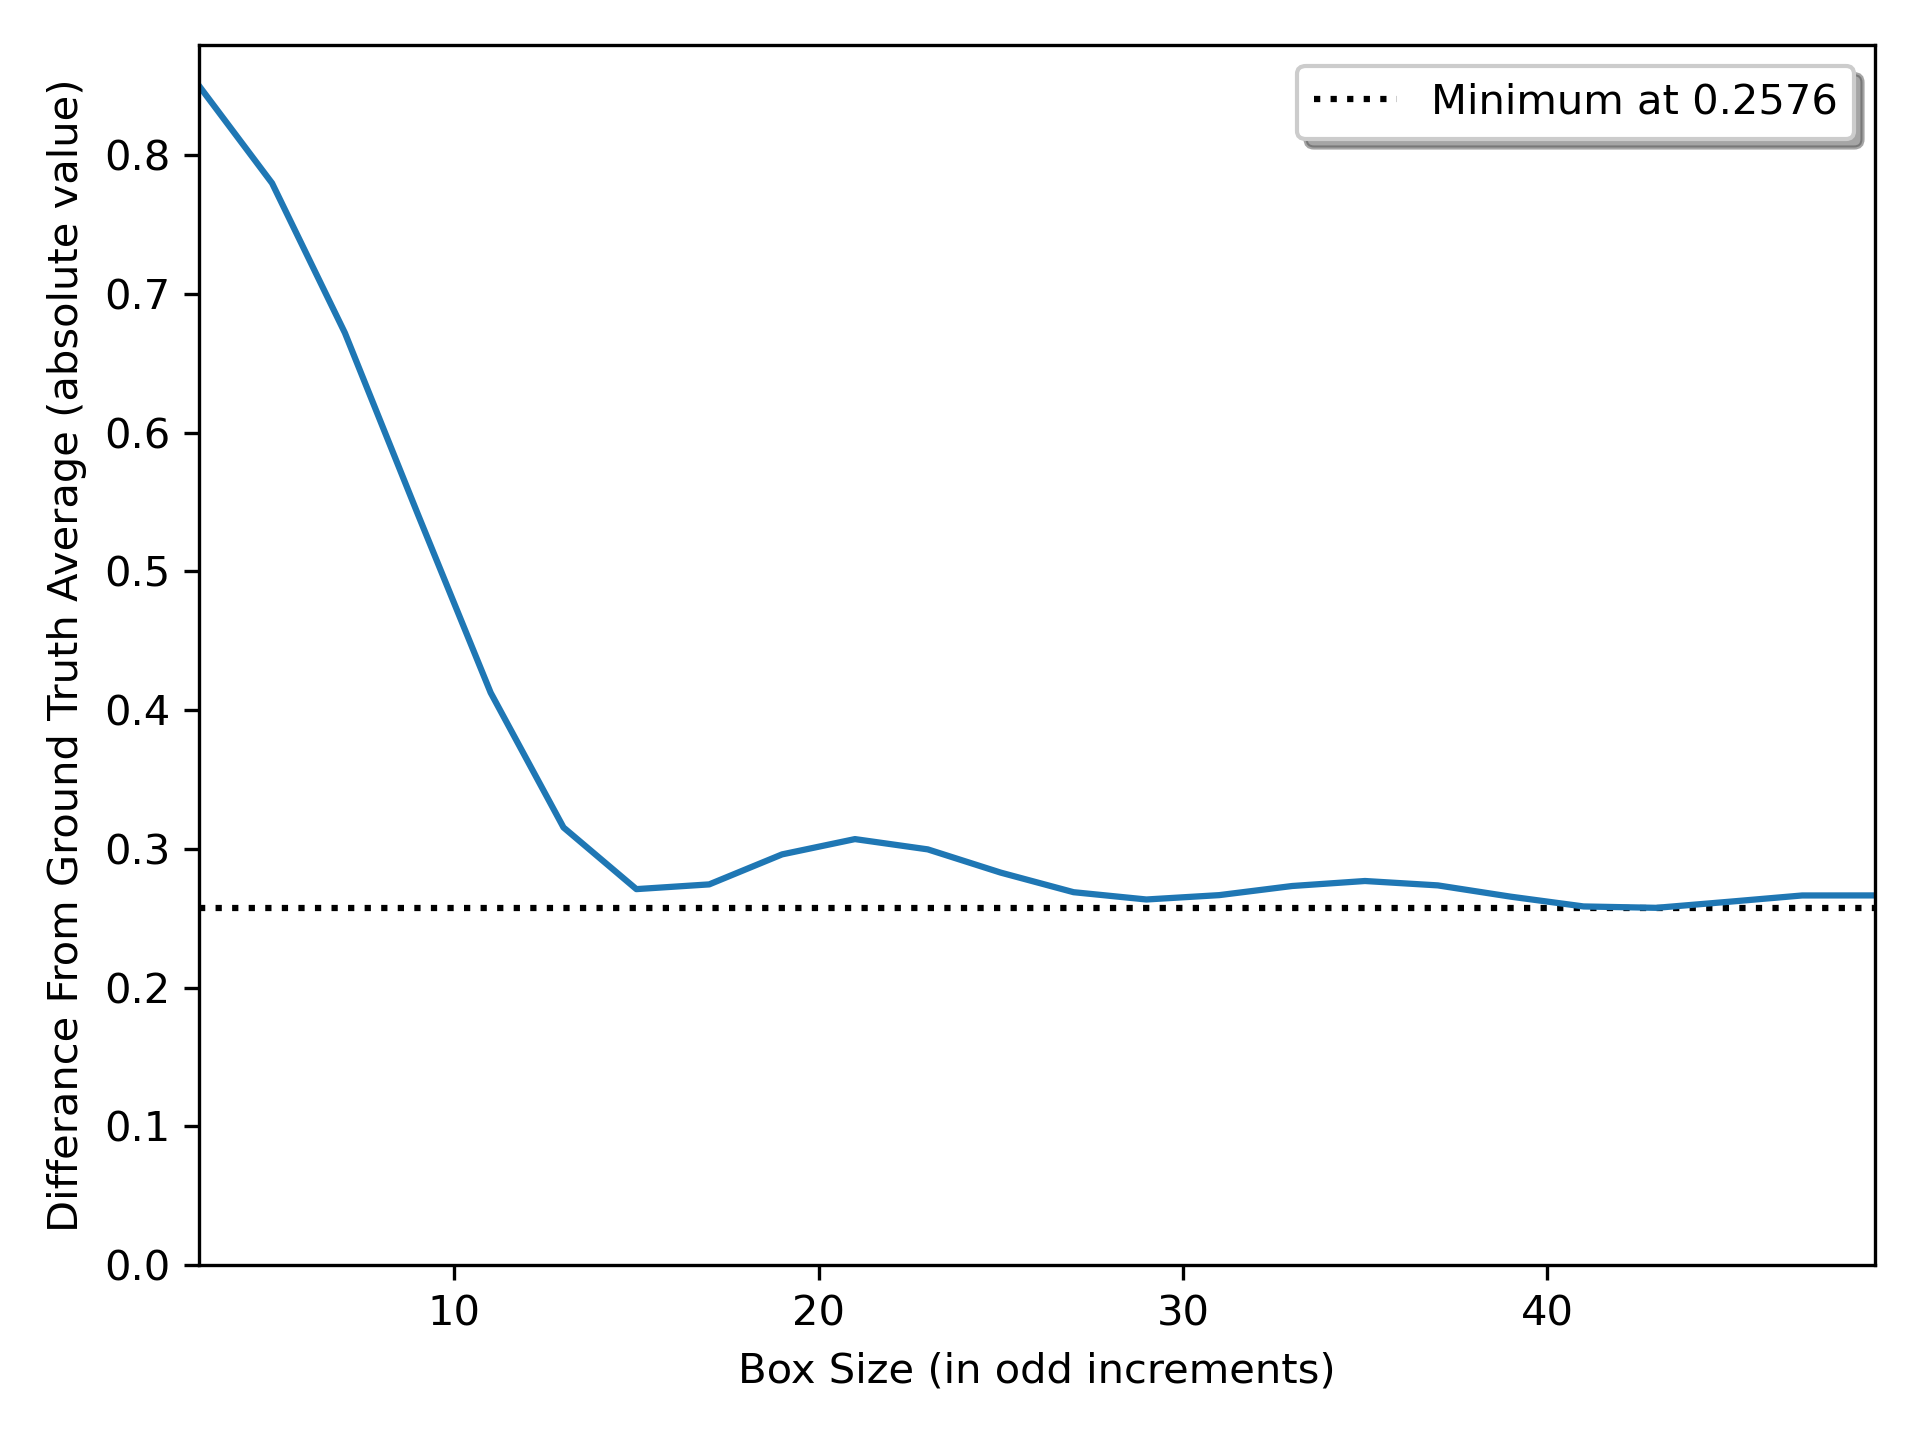
\includegraphics[width=0.7\textwidth]{project_pics/box_size_var_r8.png}
   \end{center}
   \caption{Showing the accuracy of centroiding Vs the box size chosen (from 3 to 49), for a radii or R8.00 and without noise}
   \label{fig:box_size_var_r8}
 \end{figure}

 \begin{figure}[H]
   \begin{center}
     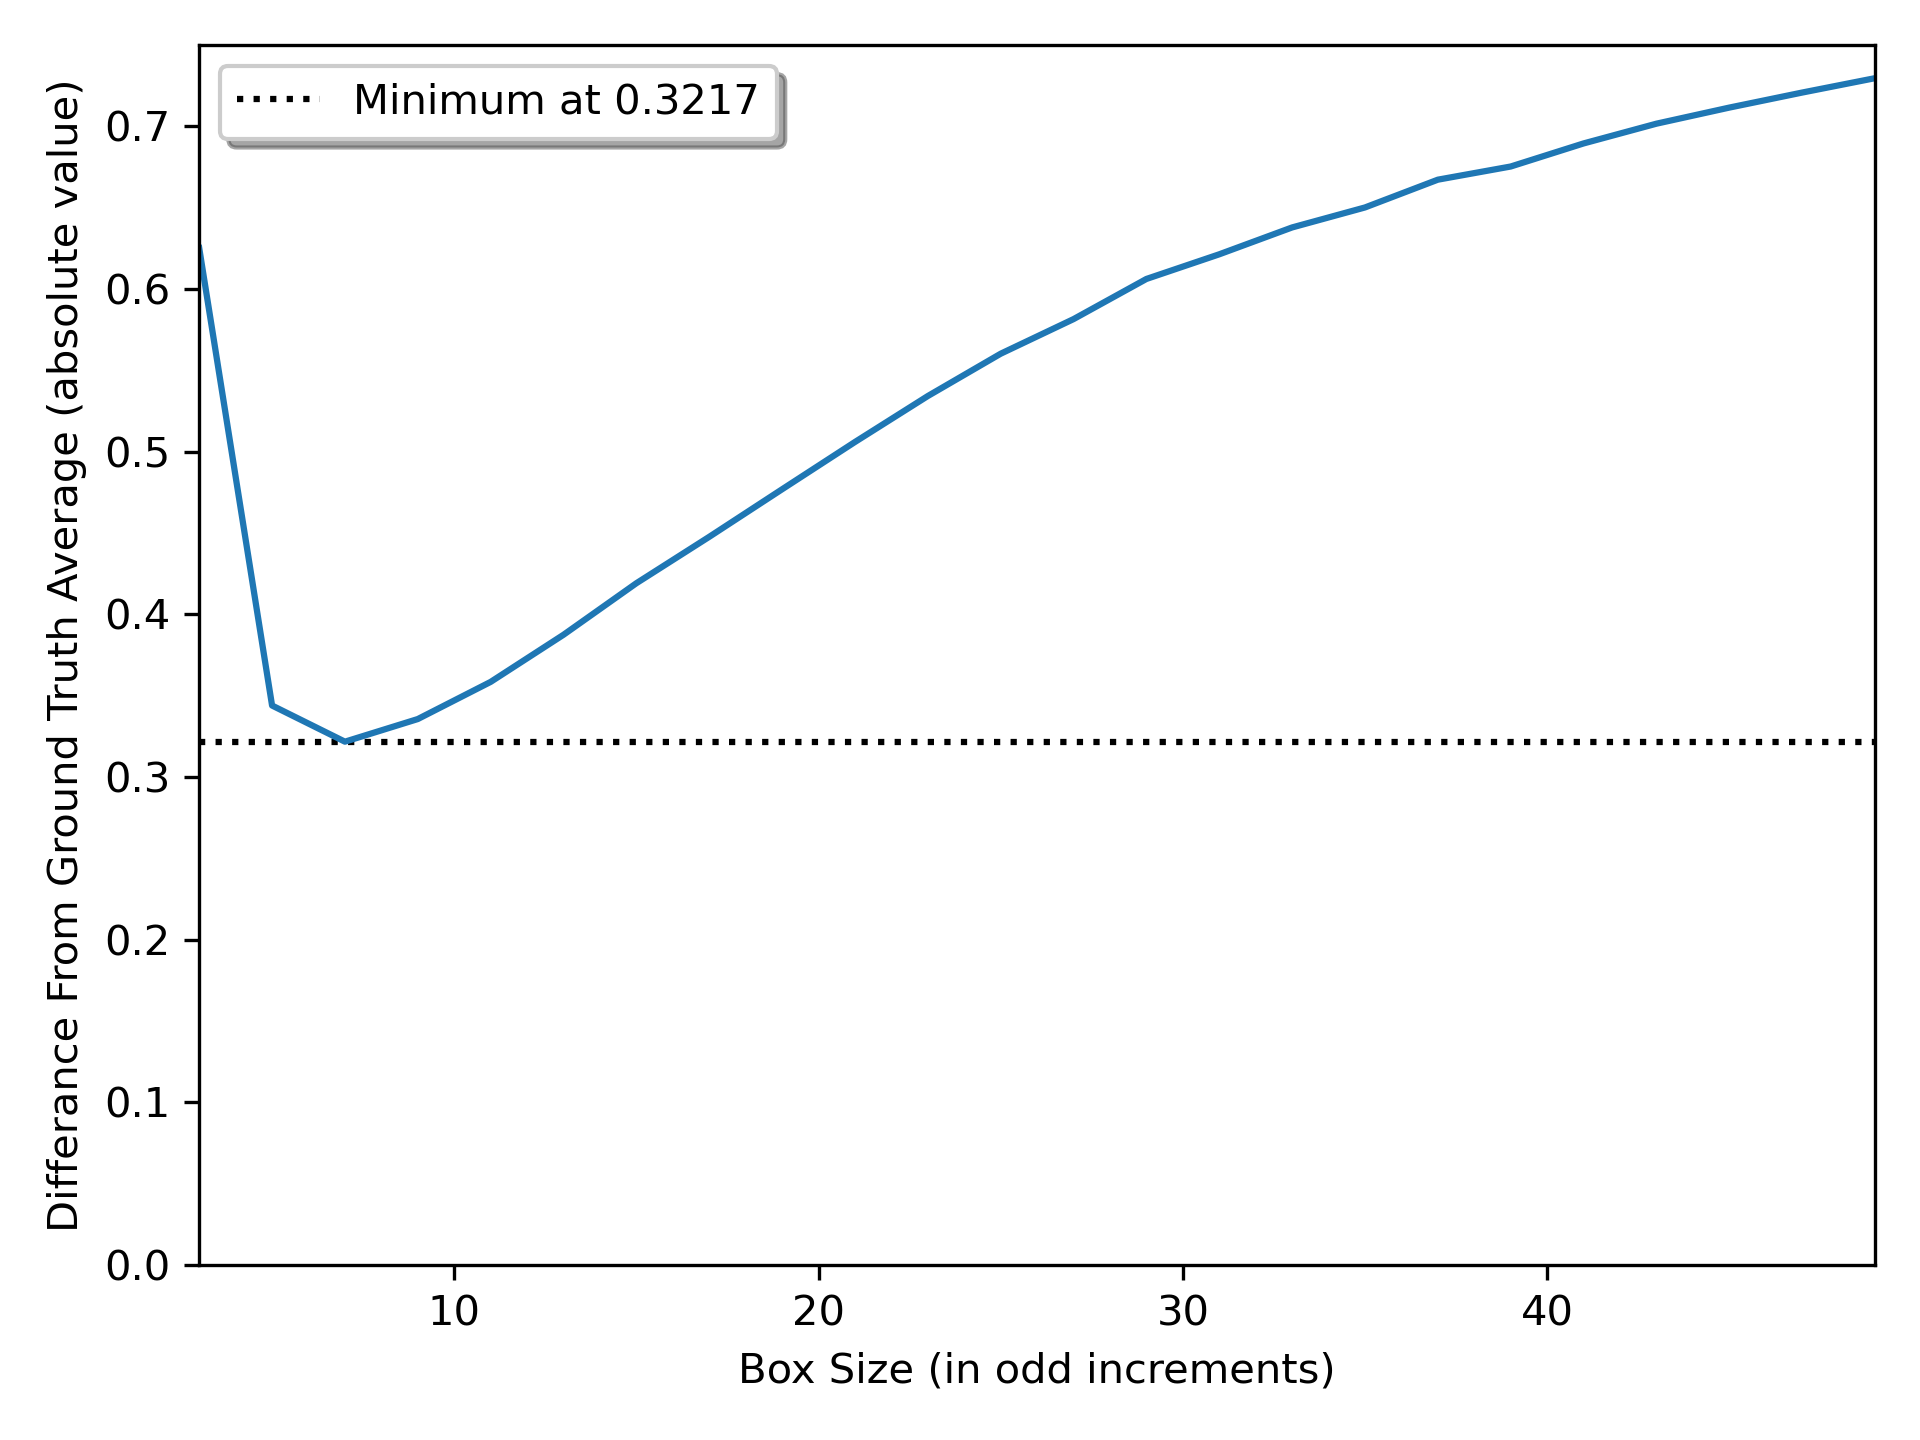
\includegraphics[width=0.7\textwidth]{project_pics/box_size_var_noise_r2.png}
   \end{center}
   \caption{Showing the accuracy of centroiding Vs the box size chosen (from 3 to 49), for a radii or R2.00 and with noise}
   \label{fig:box_size_var_noise_r2}
 \end{figure}
  
 \begin{figure}[H]
   \begin{center}
     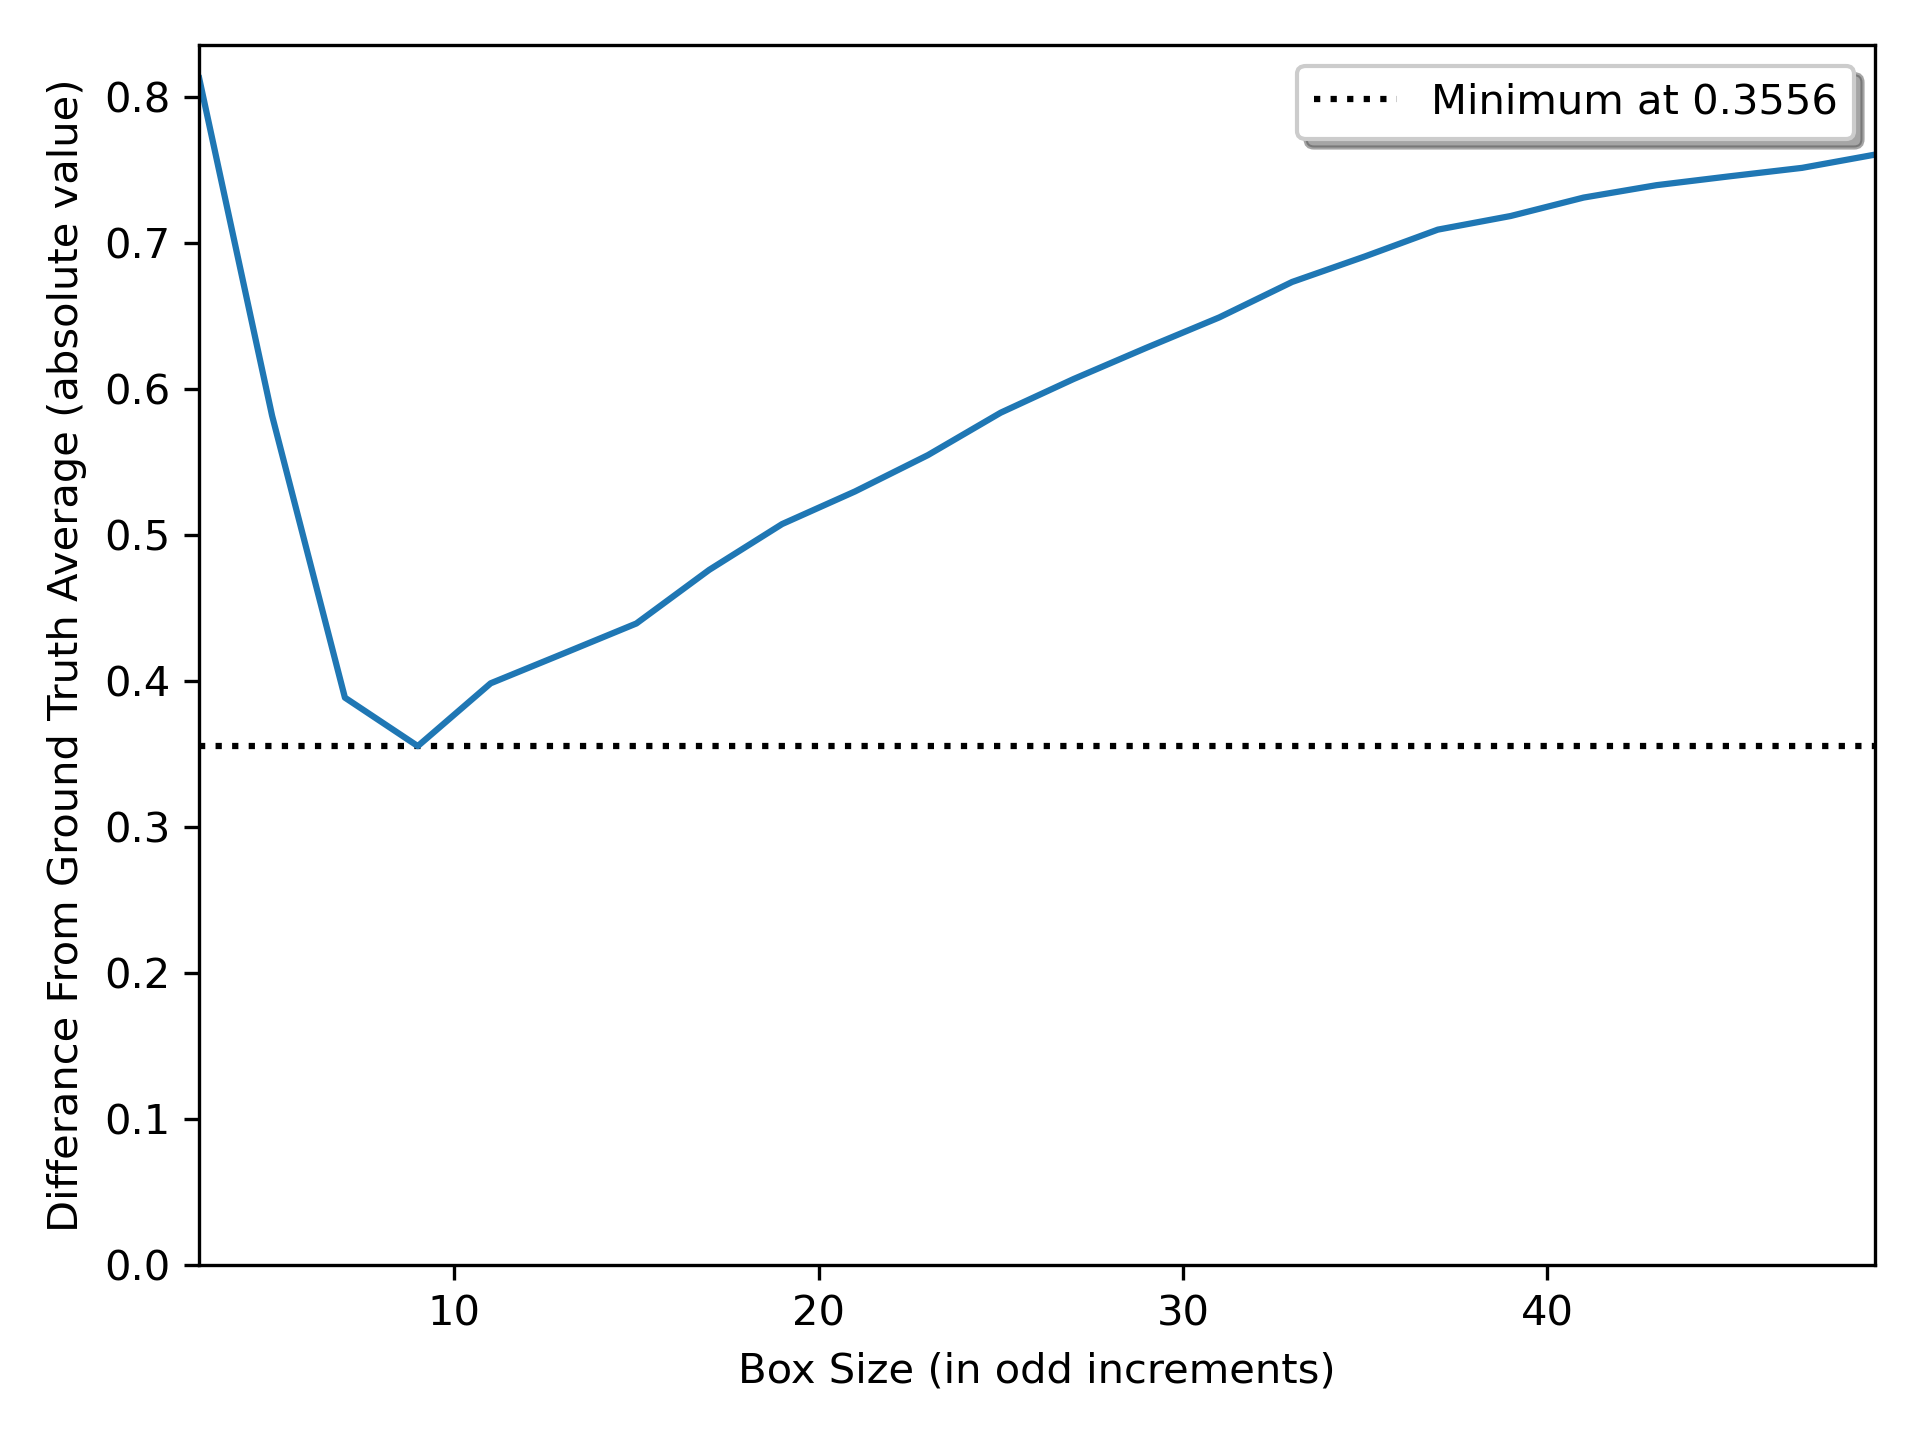
\includegraphics[width=0.7\textwidth]{project_pics/box_size_var_noise_r4.png}
   \end{center}
   \caption{Showing the accuracy of centroiding Vs the box size chosen (from 3 to 49), for a radii or R4.00 and with noise}
   \label{fig:box_size_var_noise_r4}
 \end{figure}

 \begin{figure}[H]
   \begin{center}
     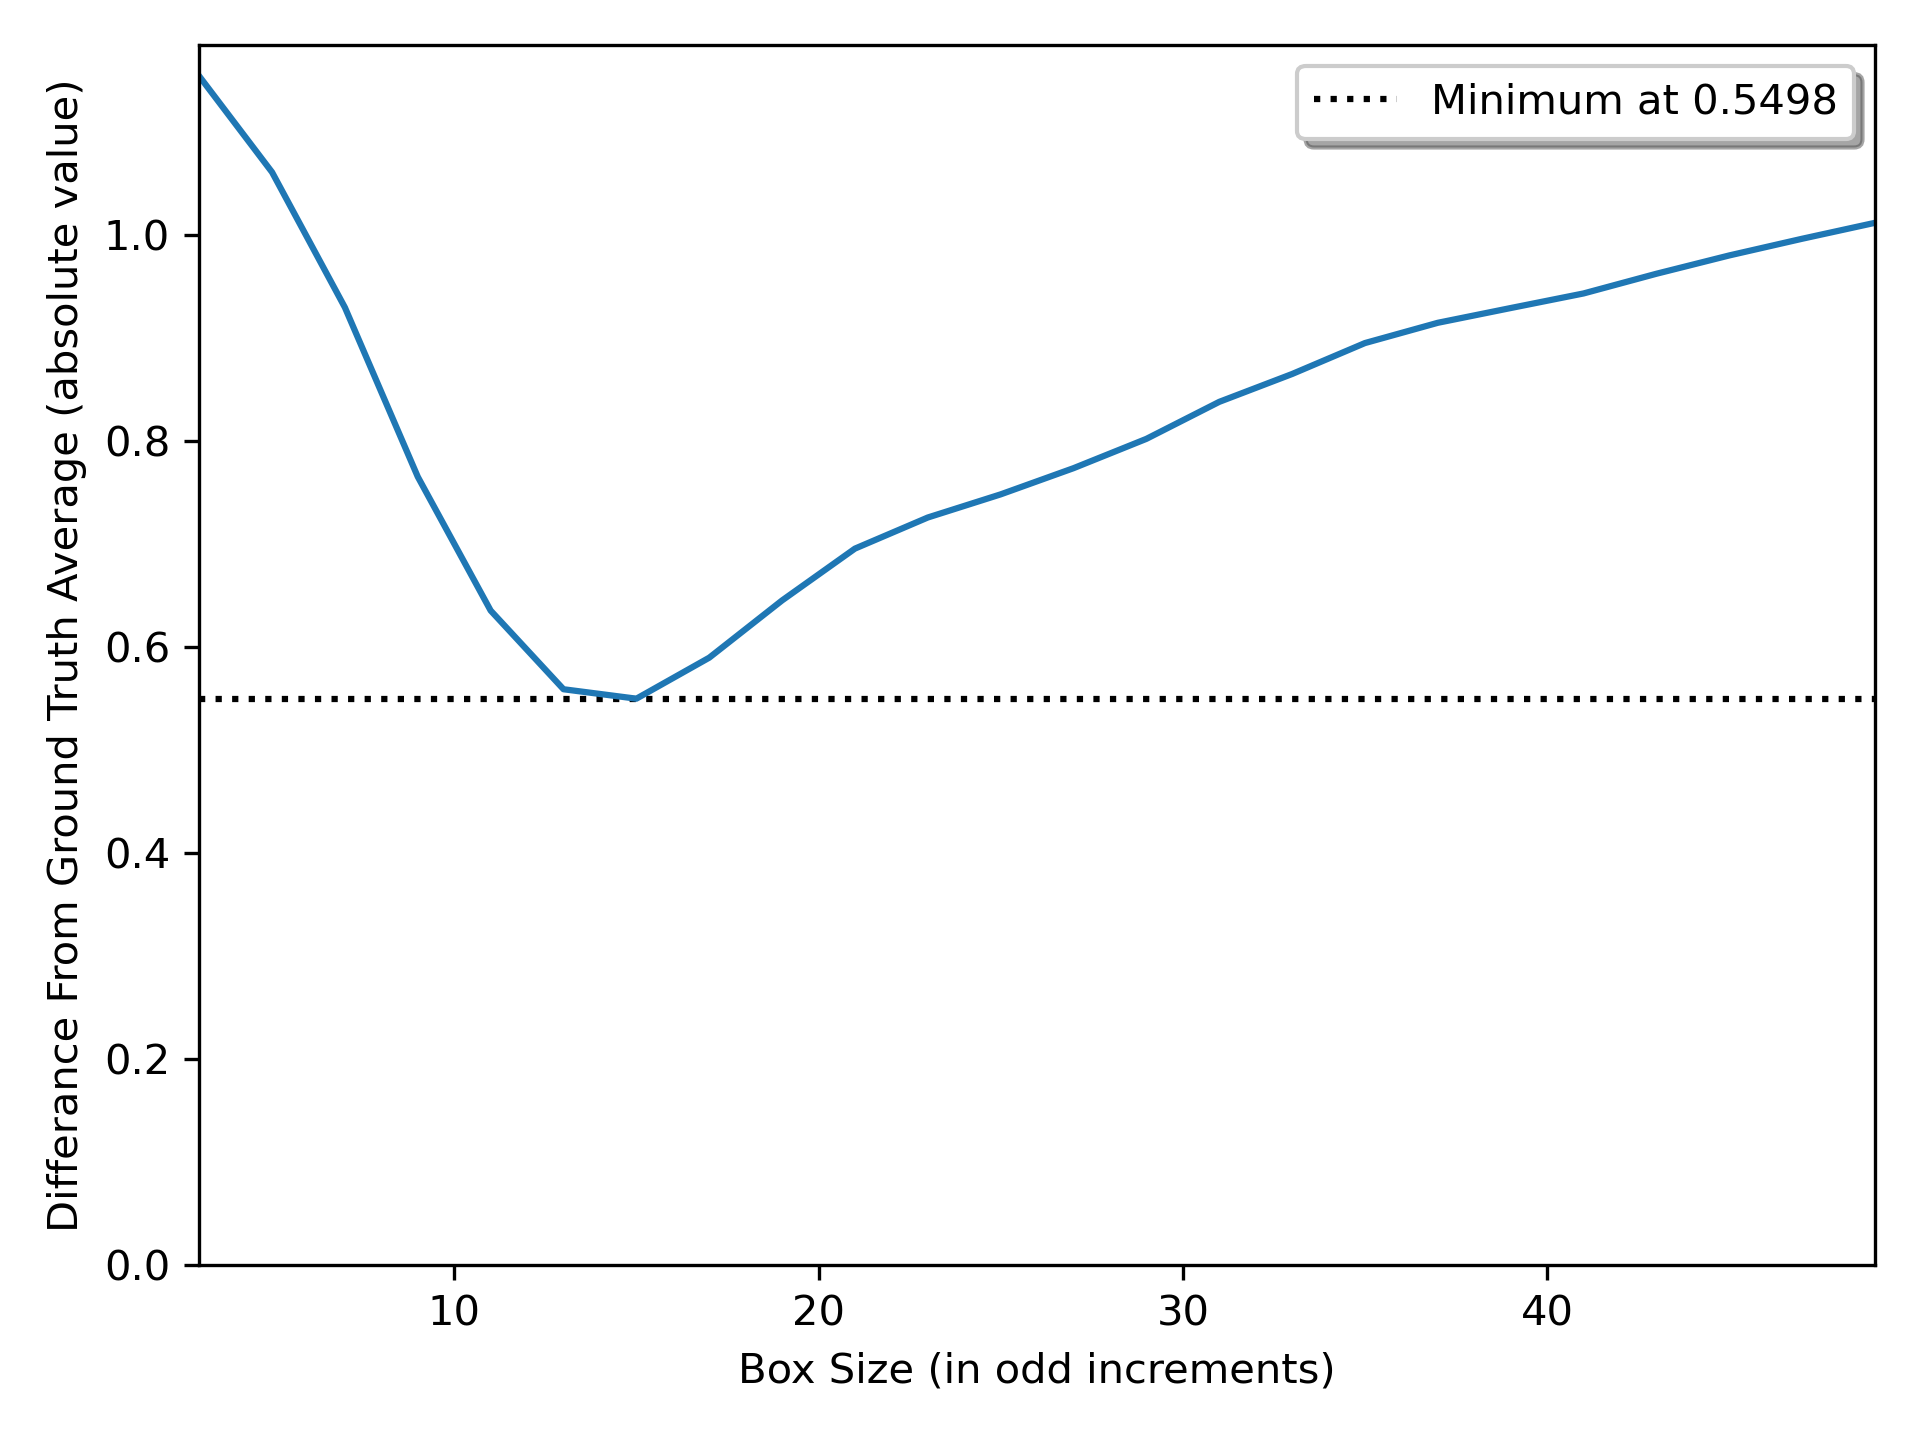
\includegraphics[width=0.7\textwidth]{project_pics/box_size_var_noise_r8.png}
   \end{center}
   \caption{Showing the accuracy of centroiding Vs the box size chosen (from 3 to 49), for a radii or R8.00 and with noise}
   \label{fig:box_size_var_noise_r8}
 \end{figure}


\end{document}
